\documentclass[
  12pt,
	openright,%
	parskip=full,
  % twoside=true,
	chapterprefix=true,%	
	headings=normal,%	
	bibliography=totoc,%
	listof=totoc,%
	titlepage=on,%
	captions=tableabove,%
	spanish,
]{scrreprt}

% ====================================
% Paquetes y Estilos
% ====================================

\usepackage{Paquetes/Paquetes}
\usepackage{Paquetes/Fuentes}
\usepackage{Paquetes/Ambientes}
\usetikzlibrary{external}
\tikzexternalize[prefix=Cache/]

% ====================================
% Datos de la tesis
% ====================================

\newcommand{\alumno}{Ángel Emmanuel Peñaflor Zetina}
\newcommand{\facultad}{Facultad de Matemáticas}
\newcommand{\region}{Región Xalapa}
\newcommand{\programa}{Licenciatura en Matemáticas}
\newcommand{\titulo}{Cálculo de Geodésicas en el Disco de Poincaré}
\newcommand{\DirectorUno}{Dr. Francisco Gabriel Hernández Zamora}
\newcommand{\DirectorDos}{Dr. Evodio Muñoz Aguirre}


% ====================================
% Documento
% ====================================

\begin{document}

% ====================================
% Portada, agradecimientos y dedicatoria
% ====================================

\pagenumbering{gobble}
\newgeometry{left=0.7cm, right=0.7cm, top=1.2cm, bottom=0.7cm} % Márgenes únicamente para esta sección.

% Logosímbolo institucional.
\tikzexternaldisable % Desactiva el precompilado de figuras, ¡No quitar!
\begin{figure}
	
\includegraphics[height=4.3cm,right=19.375cm]{Figuras/0-UV/Logo.png}
\end{figure}

% Linea bajo el logosímbolo
\begin{tikzpicture}[remember picture,overlay]
	\draw[opacity=1]($(current page.north west)+(14.9cm,-5.60cm)$)--($(current page.north west)+(20.19cm,-5.60cm)$);
\end{tikzpicture}

% Datos de la tesis.
\begin{textblock*}{15cm}(2.5cm,5cm)
	\begin{flushright}
		{\GilliusUno \facultad \\ \region}\\[12pt]
		{\GilliusDos \programa}\\[16pt]
		{\GilliusTres \titulo}\\[16pt]
		{\GilliusDos Tesis para acreditar la Experiencia Recepcional}\\[12pt]
		{\GilliusDos Presenta: \\ \textbf{\alumno}}\\[12pt]
		{\GilliusDos Directores: \\ \DirectorUno \\ \DirectorDos}\\[12pt]
		{\GilliusDos \today}\\[12pt]
		{\GilliusDos “Lis de Veracruz: Arte, Ciencia, Luz”}\\[12pt]
	\end{flushright}
\end{textblock*}

% Adorno al pie de página.
\begin{figure}[!b]
	
\includegraphics[height=9cm,left]{Figuras/0-UV/Inferior.png}
\end{figure}

% \begin{tikzpicture}[remember picture,overlay]
	\draw[,dash pattern=on 10pt off 3pt,line width=2pt]($(current page.north)+(6.795cm,0cm)$)--($(current page.south)+(6.795cm,0cm)$);

	\draw[,dash pattern=on 10pt off 3pt,line width=2pt]($(current page.north west)+(0.7cm,0cm)$)--($(current page.south west)+(0.7cm,0cm)$);

	\draw[line width=2pt,purple,latex-latex,,dash pattern=on 10pt off 3pt]($(current page.north west)+(0cm,-1.2cm)$)--($(current page.north east)+(0cm,-1.2cm)$);

	\draw[line width=2pt,purple,latex-latex,,dash pattern=on 10pt off 3pt]($(current page.north west)+(0cm,-5.5cm)$)--($(current page.north east)+(0cm,-5.5cm)$);

	\draw[line width=2pt,purple,latex-latex,,dash pattern=on 10pt off 3pt]($(current page.north west)+(0cm,-6cm)$)--($(current page.north east)+(0cm,-6cm)$);

	\draw[line width=2pt,purple,latex-latex,,dash pattern=on 10pt off 3pt]($(current page.south west)+(0cm,10.7cm)$)--($(current page.south east)+(0cm,10.7cm)$);

	\draw[line width=2pt,purple,latex-latex,,dash pattern=on 10pt off 3pt]($(current page.south west)+(0cm,9.7cm)$)--($(current page.south east)+(0cm,9.7cm)$);

	\draw[line width=2pt,purple,latex-latex,,dash pattern=on 10pt off 3pt]($(current page.south west)+(0cm,0.7cm)$)--($(current page.south east)+(0cm,0.7cm)$);
\end{tikzpicture}


\tikzexternalenable % Restaura la el precompilado de figuras.
\restoregeometry % Restaura los margenes del documento.

\begin{flushleft}
  {\GilliusSiete Universidad Veracruzana}\\[12pt]
  {\GilliusOcho \facultad \\ \region}\\[12pt]
  {\GilliusOcho \programa}\\[12pt]
  {\GilliusNueve \titulo}\\[12pt]
  {\GilliusOcho Tesis para acreditar la Experiencia Recepcional}\\[12pt]
  {\GilliusOcho Presenta: \\ \alumno}\\[12pt]
  {\GilliusOcho Directores: \\ \DirectorUno \\ \DirectorDos}\\[12pt]
\end{flushleft}



\chapter*{Agradecimientos}
\label{sec:agradecimientos}
Gracias.
\begin{center}

\includegraphics[width=0.5\textwidth]{Figuras/Gracias}
\end{center}

\chapter*{Dedicatoria}

A mi familia, a Paola y a Dios.

\cleardoublepage

% ====================================
% Tabla de Contenidos.
% ====================================

\setcounter{tocdepth}{3}
\tableofcontents
% \listoffigures
\cleardoublepage

\pagenumbering{arabic} % Esto activa la numeración de las páginas.
\pagestyle{plain} % Esto enumera cada una de las páginas, sin esto el número de página solo aparece en los cambios de sección.
\setcounter{page}{1}

% ====================================
% Variedades y Mapas
% ====================================


\chapter{Variedades y Mapas}\label{Capítulo: Variedades y Mapas}
\section{Variedades Topológicas}\label{Sección: Variedades Topologicas}
Nuestro objeto de estudio fundamental serán las \it{variedades}, estos son espacios topológicos que localmente se asemejan a espacios euclidianos. En particular nos interesan las variedades que podamos dotar de una estructura suave, esto es, las variedades en las que podemos darle un significado a la derivada.

\begin{definition}[Variedad Topológica]\label{Definición: Variedad Topologica}
	Sea $M$ un espacio topológico, diremos que $M$ es una \it{variedad topológica $n$-dimensional} si:
	\begin{enumerate}
		\item $M$ es un \it{espacio de Hausdorff}; esto es, para cualesquiera par de puntos distintos $x_1,x_2$ de $M$ existen vecindades $U_1$ y $U_2$ de $x_1$ y $x_2$ respectivamente, que son disjuntas.
		\item $M$ es \it{segundo numerable}; esto es, la topología de $M$ tiene una base numerable.
		\item $M$ es \it{localmente Euclidiano} de dimensión $n$; esto es, para cada punto $x$ de $M$ existe una vecindad abierta $U \subset M$ que contiene a $x$ y una función $\phi: U \to \R^n$ continua y con inversa continua, i.e., un \it{homeomorfismo}.
	\end{enumerate}
\end{definition}

Para abreviar escribiremos \enquote{Sea $M^n$ una variedad topológica},  en lugar de escribir \enquote{Sea $M$ una variedad topológica $n$-dimensional}. Ocasionalmente, cuando no sea relevante, omitiremos escribir la dimensión de la variedad.

\begin{figure}[h]
	\begin{center}
		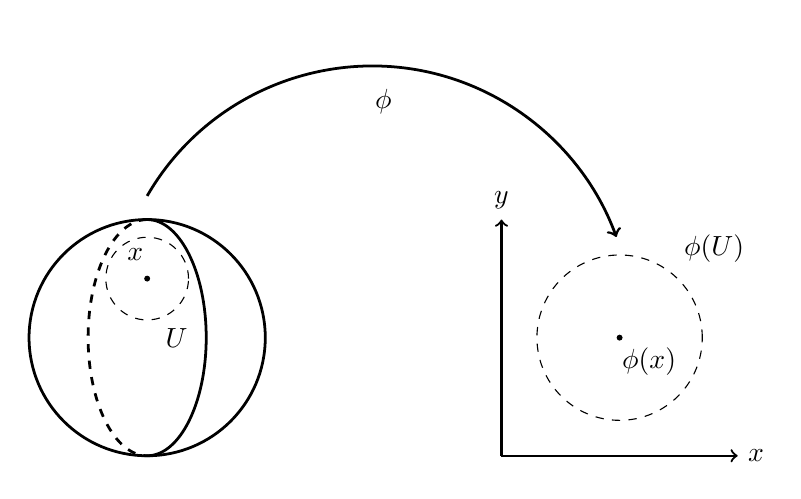
\begin{tikzpicture}[scale=1.5]
  \draw[line width=1] (-3,2) arc (90:-90:0.5 and 1);
  \draw[line width=1, dashed] (-3,2) arc (90:270:0.5 and 1);
  \draw[line width=1](-3,1) circle (1);
  \draw[color=black,thick,->] (0,0) -- (2,0) node[anchor=west]{$x$};
  \draw[color=black,thick,->] (0,0) -- (0,2) node[anchor=south]{$y$};

  \filldraw[black] (1,1) circle (0.02);
  \draw[dashed] (1,1) circle (0.7);
  \draw node at (1.25,0.80) {$\phi(x)$};
  \draw node at (1.8,1.75) {$\phi(U)$};

  \filldraw[black] (-3,1.5) circle (0.02);
  \draw node at (-3.1,1.70) {$x$};
  \draw[dashed] (-3,1.5) circle (0.35);
  \draw node at (-2.75,1) {$U$};

  \draw[line width=1, ->] (-3,2.2) arc (150:20:2.2);
  \draw node at (-1,3) {$\phi$};
\end{tikzpicture}

		\caption{Representación de un homeomorfismo de una variedad a $\R^{2}$.}
	\end{center}
\end{figure}

La definición que acabamos de dar no es única, en el sentido de que existen diferentes definiciones de lo que es una variedad, algunos autores debilitan algunas de las propiedades, por ejemplo, pidiendo que las variedades sean localmente Hausdorff, otros no piden que sean segundo numerables, y algunos otros piden que el homeomorfismo sea con una vecindad abierta de algún espacio de Banach.

Las propiedades que nosotros pedimos, como iremos viendo a lo largo de esta tesis, son bastante agradables para hacer cálculos, ya que, entre otras cosas, nos permitirán extender de manera sencilla funciones locales a toda la variedad y, eventualmente, definir esta propiedad nos permitirá definir lo que es una variedad Riemanniana.


\begin{example}[Espacios Euclidianos]\label{Ex: Variedad Topologica - Espacios Euclidianos}
	El ejemplo más sencillo de una variedad topológica es $(\R^n,d)$ donde $d$ es la función distancia usual.
	\begin{enumerate}
		\item Sabemos que es Hausdorff ya que para cualesquiera dos puntos $x_1,x_2 \in \R^n$ podemos considerar vecindades $V_r(x_1), V_r(x_2)$ donde $r < \frac{d(x,y)}{2}$ de modo que $V_r(x_1) \cap V_r(x_2) = \varnothing$.
		\item Es segundo numerable ya que las bolas abiertas con radios racionales y centros racionales forman una base numerable para la topología.
		\item Para cada $x \in \R^n$ podemos considerar a $\R^n$ como la vecindad abierta y tomar la función identidad $\id: \R^n \to \R^n$ que, trivialmente, es un homeomorfismo.
	\end{enumerate}
\end{example}

\begin{figure}[h]
	\centering
	\begin{tikzpicture}[scale=2]
	\draw[<->] (-2.5,0) -- (-1,0) node[right=3.5pt, below=-1.5pt, font=\fontsize{5pt}{5pt}]{$x$};
	\draw[<->] (-2,-0.5) -- (-2,1) node[above=3pt, font=\fontsize{6pt}{6pt}]{$y$};

	\node[black,font=\fontsize{8pt}{8pt}] at (-1.15,0.85) {$\mathbb{R}^2$};

	\draw[<->] (-0.25,0,0) -- (1.5,0,0) node[above=1pt, font=\fontsize{6pt}{6pt}]{$x$};
	\draw[<->] (0.5,-0.5,0) -- (0.5,1,0)
	node[above=3pt, font=\fontsize{6pt}{6pt}]{$y$};
	\draw[<->] (0.5,0,-1.25) -- (0.5,0,1.25) node[below=3pt,right, font=\fontsize{6pt}{6pt}]{$z$};

	\node[black, font=\fontsize{8pt}{8pt}] at (1.5,0.85) {$\mathbb{R}^3$};
\end{tikzpicture}

	\caption{$\R^2$ y $\R^3$ son variedades topológicas.}
\end{figure}

\begin{example}[Bolas Abiertas]\label{Ex: Variedad Topologica - Bolas Abiertas}
	Otro ejemplo sencillo de variedad topológica son las bolas abiertas en $(\R^n,d)$, donde nuevamente $d$ es la función distancia usual. La topología inducida en la bola hereda el ser Hausdorff y la segundo numerabilidad. Sin pérdida de generalidad podemos suponer que la bola está centrada en el origen y tomarla como la vecindad abierta, así podremos tomar la función $\phi: B_r(0) \to \R^n$ definida por:
	\[
		\phi(x) = \frac{x}{r - \|x\|}.
	\]

	Esta función tiene como inversa a la función $\phi^{-1}: \R^n \to B_r(0)$ dada por:
	\[ \phi^{-1}(y) = \frac{ry}{1 + \|y\|}.
	\]
  Dado que la función inversa existe, $\phi$ es necesariamente una biyección y como ambas funciones son diferenciables serán continuas, por lo que $\phi$ es un homeomorfismo de $B_r(0)$ sobre $\R^n$. Por lo tanto, cualquier bola abierta centrada en el origen será una variedad topológica. Existe un homeomorfismo natural entre una bola arbitraria en $\R^n$ y la bola unitaria en $\R^n$, por lo cual cualquier bola abierta en $\R^n$ será una variedad topológica.
\end{example}

\begin{figure}[h]
	\centering
	\begin{tikzpicture}[scale=4.5]
{\draw[color=black,thick,->] (0,0) -- (1,0) node[anchor=west]{$x$};}%
{\draw[color=black,thick,->] (0,0) -- (0,1) node[anchor=south]{$y$};}%
\draw[dashed] (0.5,0.5) circle (0.25);
\filldraw[black] (0.5,0.5) circle (0.02);
\end{tikzpicture}

	\caption{Una bola abierta en $\R^{2}$ es una variedad topológica.}
\end{figure}


\begin{definition}[Cartas Coordenadas]\label{Definición: Cartas Coordenadas}
	Sea $M^n$ una variedad topológica. Una \it{carta coordenada} en $M$ es un par $(U, \phi)$, donde $U$ es un subconjunto abierto de $M$ y $\phi: U \to \tilde{U}$ es un homeomorfismo de $U$ a un subconjunto abierto $\tilde{U} \subset \R^n$.
\end{definition}

Por definición de variedad topológica cada punto está contenido en el dominio de alguna carta. Dada un carta $(U,\phi)$ llamamos al conjunto $U$ el \it{dominio coordenado}, además, si $\phi(U)$ es una bola abierta en $\R^n$ llamaremos a $U$ una \it{bola coordinada}. Al homeomorfismo $\phi$ se le llama el \it{mapa coordenado (local)}, y a sus funciones componentes $(x^1,\hdots,x^n)$, definidas por $\phi(p) = (x^1(p), \hdots, x^n(p))$ se les conoce como las \it{coordenadas locales} en $U$.

Diremos que una carta $(U,\phi)$ está centrada en un punto $p \in M$ si se cumple que $\phi^{-1}(0) = p$. Geométricamente esto significa que la preimagen del punto $\{0\} \in \R^{n}$ es el punto $p$. Siempre podemos encontrar una carta centrada en $p$ ya que a la imagen de cualquier carta se le puede restar una constante.

A continuación veremos algunos ejemplos más interesantes de variedades topológicas.

\begin{example}[$n-$Esfera]\label{Ex: Variedad Topologica - Esfera}
	La $n-$esfera unitaria, denotada como $\S^n$, y definida como el conjunto:
	\[
		\S^n = \{x \in \R^{n+1}: \| x \| = 1 \}
	\]
	es una variedad topológica.

	En efecto, por ser un subespacio topológico de $\R^{n+1}$ la topología de subespacio de $\S^n$ heredará el ser Hausdorff y segundo numerable.

	Para mostrar que $\S^n$ es localmente euclidiana utilizaremos su proyección sobre el hiperplano $\R^{n}$. Para cada índice $i=1, \hdots, n+1$ definiremos los siguientes subconjuntos de $\S^n$:
	\begin{align*}
		U_{i}^{+} & = \{(x_1,\hdots,x_{n+1}) \in \R^{n+1}: x^i > 0\}, \\
		U_{i}^{-} & = \{(x_1,\hdots,x_{n+1}) \in \R^{n+1}: x^i < 0\}.
	\end{align*}

	Notemos que tendremos $2n + 2$ de estos subconjuntos de $\S^n$ y que estos cubrirán a $\S^n$. Sean $\pi_i: \R^{n+1} \to \R^n$ las funciones proyección que omiten la $i-$ésima coordenada, esto es,
	\[
		\pi_i(x_1,\hdots,x_i,\hdots,x_{n+1}) = (x_1,\hdots,x_{i-1},x_{i+1}\hdots,x_{n+1}).
	\]

	La imagen de cualquier conjunto $U_{i}^{\pm}$ bajo $\pi_i$ será un subconjunto de la bola unidad $\B^n$ en $\R^n$, esto dado que para cualquier $x=(x_1, \hdots, x_{n+1}) \in U_{i}^{\pm}$ se tiene que
	\[
		\|\pi_i(x)\| = \sqrt{\sum_{j=1, j\neq i}^{n+1} x_j^2} < \sqrt{\sum_{j=1}^{n+1} x_j^2} = 1.
	\]

	Ahora definamos funciones $\phi_i^{\pm}: \B^n \to \R^{n+1}$ como sigue, para cada $y=(y_1, \dots, \hat{y_i}, \dots, y_n) \in \B^n$, donde $\hat{y_i}$ significa que no estamos considerando el $i-$ésimo termino:
	\[
		\phi_{i}^{\pm}(y_1, \hdots, y_n) =  (y_1, \hdots, y_{i-1}, \pm\sqrt{1 - \|y\|^2}, y_{i+1}, \hdots, y_{n+1}).
	\]

	Dado que $\|y\| < 1$ la función estará bien definida para cada $y \in \B^n$ y además:
	\begin{align*}
		\|\phi_i^{\pm}(y)\| & = (1 + \| y \|^{2}) + \sum_{\substack{j=1, \\ j \neq i}}^{n+1} y_j^2 \\
		                    & = \left(
		1 - \sum_{\substack{j=1,                                         \\ j \neq i}}^{n+1} y_j^2
		\right) + \sum_{\substack{j=1,                                   \\ j \neq i}}^{n+1} y_j^2 \\
		                    & = 1.
	\end{align*}

	Por lo que $\phi_i^{\pm}(\B^n) \subset U_{i}^{\pm}$. Si ahora consideramos las restricciones $\tau_i^{\pm} = \pi_i |_{U_i^{\pm}}: U_i^{\pm} \to \B^n$ tendremos que $\tau_i^{\pm} \circ \phi_i^{\pm} = \id_{\B^n}$ y $\phi_i^{\pm} \circ \tau_i^{\pm} = \id_{U_i^{\pm}}$. Esto demostraría que existe una biyección entre cada uno de los conjuntos $U_i^{\pm}$ y la bola unidad $\B^n$ en $\R^n$, además de esto, tanto $\tau_i^{\pm}$ como $\phi_i^{\pm}$ son funciones continuas por lo que serán homeomorfismos, y, como cada $x \in S^n$ está contenido en algún $U_i^{\pm}$, concluimos que $\S^n$ es una variedad topológica de dimensión $n$.
\end{example}

\begin{figure}[h!]
	\centering
	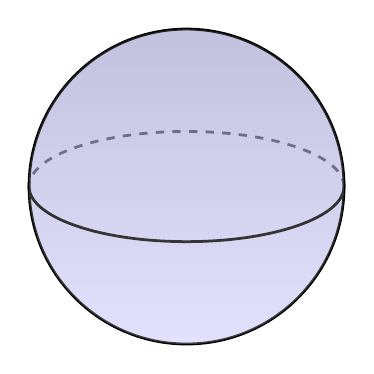
\begin{tikzpicture}[scale=2]
  \draw[line width=1, dashed] (1,0) arc (0:180:1 and 0.35);
  \draw[fill=blue!30!white!,opacity=0.5] (0,0) circle (1);
  \draw[line width=1] (1,0) arc (0:180:1 and -0.35);
  \draw[line width=1](0,0) circle (1);
  \shade[opacity=0.25] (0,0) circle (1);
\end{tikzpicture}


	\caption{La esfera $\S^{2}$ es una variedad topológica.}
\end{figure}

\begin{example}[Producto Finito de Variedades]\label{Ex: Variedad Topologica - Producto de Variedades}
	Si $M_1, \hdots, M_k$ son variedades topológicas de dimensiones $n_1,\hdots,n_k$ respectivamente, entonces $M = \Pi_{i=1}^k M_i$ es una variedad topológica de dimensión $\sum_{i=1}^k n_i$.

	En efecto, comencemos considerando el caso del producto de dos variedades. Sean $M_{1}^{n_1}$ y $M_{2}^{n_2}$ variedades topológicas. Como el producto arbitrario de espacios de Hausdorff es Hausdorff, tendremos que $M_1 \times M_2$ es Hausdorff. Además, como el producto numerable de espacios segundo numerables es segundo numerable $M_1 \times M_2$ es segundo numerable.
	Para cada punto $(x,y) \in M_1 \times M_2$ existirá un conjunto abierto $U \times V$ donde $U$ es el dominio de una carta $(U,\phi)$ en $M_1$ que contiene que a $x$ y $V$ es el dominio de una carta $(V,\psi)$ que contiene a $y$, por definición de cartas coordenadas $\phi: U \to \R^{n_1}$ y $\psi: V \to \R^{n_2}$ son homeomorfismo, por lo que podemos definir la función $F: U \times V \to \R^{n_1 + n_2}$ como:
	\[
		F(x,y) = (\phi(x),\psi(y)).
	\]

	Dado que $\phi$ y $\psi$ son homeomorfismo en particular serán funciones continuas, por lo que podemos garantizar que $F$ es continua y además es invertible, en particular, su inversa estará dada por $F^{-1}(a,b) = (\phi^{-1}(a),\psi^{-1}(b))$ y como las inversas de $\phi$  y $\psi$ también son continuas $F^{-1}$ es un mapa continuo. Así, $F$ es un homeomorfismo de $U \times V$ sobre $\R^{n_1 + n_2}$, como esto se cumple para cada punto $(x,y) \in M_1 \times M_2$ podemos concluir que el producto $M_1 \times M_2$ es una variedad topológica.

	El caso para el producto finito de variedades topológicas se sigue por inducción.
\end{example}

\begin{example}[$n-$Toro]\label{Ex: Variedad Topologica - Toro}
	El toro $n$-dimensional, que se denota por $\T^n$, y que se define como:
	\[
		\T^n = \underbrace{\S^1 \times \hdots \times \S^1}_{n-\text{veces}}.
	\]

	Esto se puede ver a partir de los ejemplos \ref{Ex: Variedad Topologica - Esfera} y \ref{Ex: Variedad Topologica - Producto de Variedades}, ya que son el producto finito de variedades topológicas.
\end{example}

\begin{figure}[h]
	\centering
	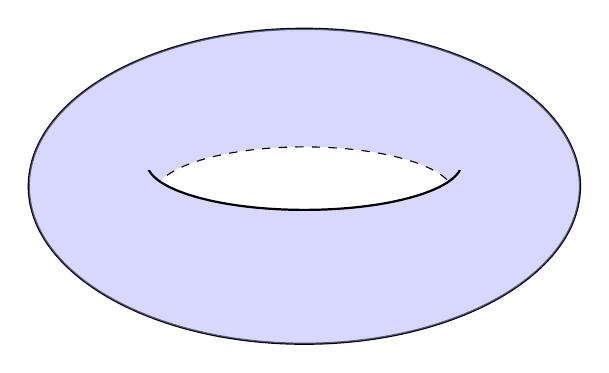
\begin{tikzpicture}[scale=2]
  % Elipse Principal
	\draw [thick] (0,0) ellipse  (1.75 and 1);
	\path[fill=blue!30!white,opacity=0.5] (0,0) ellipse  (1.75 and 1);

	%Arco inferior
	\begin{scope}
		\clip (0,0.15) ellipse (1 and 0.3);
		\fill[white] (0,-0.05) ellipse (0.95 and 0.3);
	\end{scope}

	% Arco superior
	\begin{scope}
		\clip (-1.25,0.03) rectangle (1.25,0.5);
		\draw[dashed] (0,-0.05) ellipse (0.95 and 0.3);
	\end{scope}

  % Centro
	\begin{scope}
		\clip (-1.25,0.1) rectangle (1.25,-0.5);
		\draw[thick] (0,0.15) ellipse (1 and 0.3);
	\end{scope}
\end{tikzpicture}

	\caption{El toro $\mathbb{T}^{2}$ es una variedad topológica.}
\end{figure}

\cleardoublepage
\section{Variedades Suaves}\label{Sección: Variedades Suaves}
Las variedades topológicas tienen propiedades muy interesantes en sí mismas, sin embargo, para nuestros fines lo que nos interesa es poder realizar cálculos en ellas, en particular darle sentido a la noción de diferenciabilidad. Esto no es posible en general, es con este fin que daremos algunas definiciones que nos permitirán construir una estructura adicional con la cual podremos dotar a algunas variedades topológicas; esta estructura será lo que nos permitirá dar sentido a la derivada.

Cuando decimos que una función $f$ es diferenciable o suave lo que queremos decir es que: Si $U$ y $V$ son subconjuntos abiertos de $\R^n$ y $\R^m$ respectivamente, entonces  $f: U \to V$ tiene derivadas parciales de todos los órdenes. Al conjunto de funciones con esta propiedad usualmente se le denota como $C^{\infty}$ y se dice que las funciones son de clase $C^{\infty}$.


\begin{definition}[Mapa de Transición]\label{Definición: Mapa de Transición}
	Sea $M^n$ una variedad topológica y $(U,\phi)$, $(V,\psi)$ cartas en $M$. Si $U \cap V \neq \varnothing$, entonces a la composición $\psi \circ \phi^{-1}: \phi(U \cap V) \to \psi(U \cap V)$ es llamada el \it{mapa de transición de $\phi$ a $\psi$}
\end{definition}

\begin{definition}[Cartas Suavemente Compatibles]\label{Definición: Cartas Suavemente Compatibles}
	Diremos que dos cartas $(U,\phi)$ y $(V,\psi)$ son \it{suavemente compatibles} o $C^{\infty}-$compatibles si $U \cap V = \varnothing$ o si los mapas de transición
	\[ \psi \circ \phi^{-1}: \phi(U \cap V) \to \psi(U \cap V), \quad \phi \circ \psi^{-1}: \psi(U \cap V) \to \phi(U \cap V) \]
	son ambos suaves.
\end{definition}

\begin{figure}[h]
	\centering
	\begin{tikzpicture}[scale=1]
	\coordinate (a) at (0,0);
	\path[draw,use Hobby shortcut,closed=true,thick]
	(0,2.5) .. (2,2.5) .. (1,4.5) .. (.3,4.5) .. (-1,4) .. (-2,2.5);

	\begin{scope}
		\clip (0.25,3.5) circle (0.5);
		\fill[blue!30!white,opacity=0.5] (-0.25,3.25) circle (0.5);
	\end{scope}
	\draw[dashed] (0.25,3.5) circle (0.5);
	\draw[dashed] (-0.25,3.25) circle (0.5);
	\draw node at (0.8,4) {$V$};
	\draw node at (-0.9,2.75) {$U$};

	\draw [thick, <->] (-5,0) -- (-1,0);
	\draw [thick, <->] (-3,-2) -- (-3,2);
	\draw [thick, <->] (1,0) -- (5,0);
	\draw [thick, <->] (3,-2) -- (3,2);

	\begin{scope}
		\clip (-3,0.5) ellipse  (0.8 and 1);
    \fill[color=blue!30!white,opacity=0.5] (-2.5,0) ellipse  (1.2 and 0.8);
	\end{scope}
	\draw [dashed,thick] (-3,0.5) ellipse  (0.8 and 1);
	% \draw [dashed,thick] (-2.5,0) ellipse  (1.2 and 0.8);

	\begin{scope}
		\clip (3,0.5) ellipse  (0.8 and 1);
		\fill[color=blue!30!white,opacity=0.5](3.5,0) ellipse  (1.2 and 0.8);
	\end{scope}
	% \draw [dashed,thick] (3,0.5) ellipse  (0.8 and 1);
	\draw [dashed,thick] (3.5,0) ellipse  (1.2 and 0.8);

	\draw[line width=1, ->] (1,3.75) arc (90:-5:2.5);
	\draw[line width=1, ->] (-1,3.25) arc (-90:0:-1.5);
	\draw[line width=1, ->] (-1.75,0.5) -- (2,0.5);

	\draw node at (-2.5,2.75) {$\phi$};
	\draw node at (3.25,3) {$\psi$};
	\draw node at (-4.25,1.25) {$\phi(U)$};
	\draw node at (4.5,1) {$\psi(V)$};
	\draw node at (0.25,1) {$\psi \circ \phi^{-1}$};


\end{tikzpicture}

	\caption{Mapa de Transición}
\end{figure}

Verificar que dos cartas son suavemente compatibles es relativamente sencillo, dado que el mapa de transición es una composición de homeomorfismos este será un homeomorfismo, así, únicamente habrá que verificar que la función y su inversa son diferenciables.

\begin{definition}[Atlas, Atlas Suave y Atlas Maximal]\label{Definición: Atlas}
	Sea $M$ una variedad topológica. Un \it{atlas} en $M$, denotado como $\A$, es una colección indexada $\{(U_i,\phi_i)\}_{i\in I}$ de cartas en $M$ que cubren a la variedad, esto es:
	\[\bigcup_{i \in I} U_i = M \]

	Si cualesquiera dos cartas en un atlas son suavemente compatibles, entonces diremos que el atlas es un \it{atlas suave}. A las cartas que forman a un atlas suave se les llama \it{cartas suaves}.

	Un atlas $\A$ estará contenido en otro atlas $\mathcal{B}$ si cada carta $(U,\phi)$ que pertenece a $\A$ también pertenece a $\mathcal{B}$. Diremos que un atlas suave $\A$ es \it{maximal} si no está propiamente contenido en ningún atlas más grande.
\end{definition}

\begin{definition}[Variedad Suave]\label{Definición: Variedad Suave}
	Sea $M$ una variedad topológica. Una \it{variedad suave} será un par $(M, \A)$, donde $\A$ es un atlas maximal en $M$. Usualmente a $\A$ se le llama la \it{estructura suave} en $M$.
\end{definition}

Por conveniencia, en lugar de escribir \enquote{Sea $(M,\A)$ una variedad suave} diremos simplemente \enquote{Sea $M$ una variedad suave}; esto cuando la estructura suave se pueda entender a partir del contexto o no sea necesario referirnos a ella de forma explícita.


Si quisiéramos definir una función $f: M \to \R$ como suave, quizá pudiésemos haber estado inclinados a dar la siguiente definición: \enquote{Una función $f: M \to \R$ es diferenciable si y sólo si para cada carta $(U,\phi)$ se tiene que $f\circ \phi^{-1}: \phi(U) \to \R$ es una función diferenciable}, esta definición podría parecernos más natural, sin embargo, presenta un problema de ambigüedad ya que, para una misma variedad pueden existir muchos atlas diferentes que generan estructuras similares pero distintas, como veremos en los siguientes ejemplos.

\begin{figure}[h]
	\begin{center}
		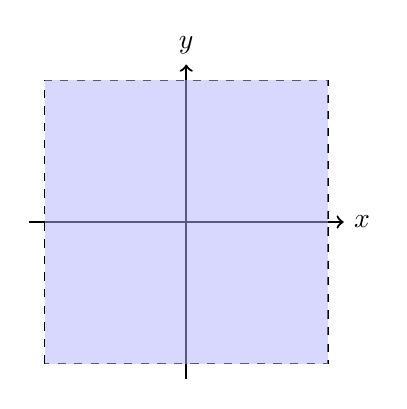
\begin{tikzpicture}[scale=2, baseline={(0,-1.5)}]
\draw[color=black,thick,->] (-1,0) -- (1,0) node[anchor=west]{$x$};%
\draw[color=black,thick,->] (0,-1) -- (0,1) node[anchor=south]{$y$};%

\draw[dashed] (-0.90,-0.90) rectangle (0.90,0.90);
\path[fill=blue!30!white,opacity=0.5] (-0.90,-0.90) rectangle (0.90,0.90);

\end{tikzpicture}

		\caption{Representación de $\R^2$ siendo cubierta por una única carta.}
	\end{center}
\end{figure}

\begin{example}[Variedades Cubiertas Por Una Única Carta]\label{Ex: Variedad Suave - Carta Unica}
	Si $M^n$ es una variedad topológica y existe un atlas para $M$ que contiene a una única carta entonces la carta define una estructura suave para la variedad, esto dado que trivialmente cumplirá el ser suavemente compatible con cualquier otra carta en el atlas.
\end{example}


\begin{example}[Espacios Euclidianos]\label{Ex: Variedad Suave - Espacios Euclidianos}
	Si tomamos cualquier espacio Euclidiano $\R^n$ podemos dar el atlas formado únicamente por la carta $(\R^n,\id_{\R^n})$, por el ejemplo anterior sabemos que esta carta define una estructura suave en $\R^n$.
\end{example}

\begin{example} % Ejemplo de diferentes estructuras suaves.
	Podemos considerar la función $\psi: \R \to \R$, definida del siguiente modo:
	\[
		\psi(x) = x^3
	\]

	Esta función es un homeomorfismo, y por los ejemplos anteriores sabemos que $(\R, \psi(x))$ es una variedad suave, con la estructura definida por  $\psi$. Sin embargo, al considerar el mapa de transición tenemos que $\id_{\R} \circ \psi^{-1}(y) = y^{\frac{1}{3}}$, y esta función no es diferenciable en el origen, por lo cual las cartas no son suavemente compatibles, y las estructuras determinadas por $(\R, \id_{\R})$ y $(\R,\psi)$ serán diferentes.
\end{example}

Para resolver este problema de ambigüedad es que hemos introducido el concepto atlas maximal. Lo que el atlas maximal nos garantiza es que cada carta que sea suavemente compatible con cualquier otra carta en el atlas estará ya incluida en el mismo.

\begin{theorem}
	Si $M$ es una variedad topológica, entonces cada atlas suave $\A$ de $M$ está contenido en un atlas suave maximal único, llamado la \it{estructura suave determinada por $\A$}.
\end{theorem}

\begin{proof}
	Sea $\A$ un atlas suave para $M$ y sea $\bar{\A}$ el conjunto de todas las cartas que son suavemente compatibles con todas las cartas de $\A$.
	\begin{enumerate}
		\item $\bar{A}$ es un atlas suave. Consideremos dos cartas arbitrarias $(U,\phi)$ y $(V,\psi)$ en $\bar{\A}$, además consideremos un punto arbitrario $\phi(p) \in \phi(U \cap V)$. Por definición el atlas $\A$ cubre a $M$, por lo que existirá una carta $(W,\theta)$ en $\bar{A}$ tal que $p \in W$, por construcción de $\bar{A}$ sabemos que $\psi \circ \theta^{-1}$ y $\theta \circ \phi^{-1}$ son suaves. Y, dado que $p \in U \cap V \cap W$, se sigue que $\psi \circ \phi^{-1} = (\psi \circ \theta^{-1}) \circ \theta \circ \phi^{-1}$, al ser una composición de funciones suaves será suave en $\phi(U \cap V)$, dado que hemos elegido las cartas $(U,\phi)$ y $(V,\psi)$ de manera arbitraria podemos concluir que $\bar{\A}$ es un atlas suave.
		\item $\bar{\A}$ es un atlas maximal. Si consideramos una carta que sea suavemente compatible con cualquier otra carta en $\bar{\A}$ por construcción esta carta deberá ser suavemente compatible con cualquier otra carta en $\A$, pero esto implica que la carta pertenece a $\bar{\A}$, por lo tanto $\bar{\A}$ es maximal.
		\item $\bar{\A}$ es único. Tomando algún otro atlas suave maximal $\mathcal{B}$ que contenga a $\A$ tendremos que cada una de sus cartas es suavemente compatible con cada carta en $\A$ por lo que $\mathcal{B} \subseteq \bar{\A}$, pero al ser $\mathcal{B}$ maximal se tendrá que $\mathcal{B} = \bar{A}$
	\end{enumerate}
\end{proof}

\begin{theorem}\label{Teorema: Unicidad de Estructura Suave}
	Dos atlas suaves para una variedad $M$ determinan la misma estructura suave si y sólo si su unión es un atlas suave.
\end{theorem}

\begin{proof}
	Sean $\A$ y $\mathcal{B}$ dos atlas suaves en $M$ y que ambos determinan la misma estructura suave. Por el teorema anterior sabemos que esto significa que existe un atlas suave maximal $\mathcal{C}$ tal que $\A \subset \mathcal{C}$ y $\mathcal{B} \subset \mathcal{C}$.

	Si consideramos una carta $(U,\phi) \in \A \cup \mathcal{B}$ esta deberá estar contenida en $\A$ o $\mathcal{B}$, podemos suponer sin pérdida de generalidad que está contenida en $\A$, también estará contenida en $\mathcal{C}$ y por construcción cada carta en $\mathcal{C}$ debe ser suavemente compatible con cada carta en $\mathcal{B}$, análogamente para el caso en que la carta está contenida en $\mathcal{B}$. Por lo tanto, podemos concluir que $\A \cup \mathcal{B}$ es un atlas suave.

	Supongamos ahora que $\A \cup \mathcal{B}$ es un atlas suave. Dado que las estructuras suaves determinadas por $\A$ y $\mathcal{B}$ ambas contendrán a $\A \cup \mathcal{B}$, y que por el teorema anterior hay una única estructura suave que contiene a $\A \cup \mathcal{B}$ podemos concluir que $\A$ y $\mathcal{B}$ determinan la misma estructura suave.
\end{proof}

Lo que estos dos teoremas nos permiten hacer es definir de manera más sencilla la estructura suave para una variedad, ya que, en lugar de tener que describir un atlas maximal podemos simplemente escoger algún atlas suave y sabemos que la estructura determinada será única.

Hay muchos ejemplos de variedad suaves y, como veremos a continuación, a cada una de las variedades topológicas que dimos como ejemplo anteriormente se le puede dar una estructura suave, sin embargo, esto no es cierto en general, hay ejemplos de variedades topológicas a las cuales no se les puede dar una estructura suave. Un resultado interesante que no veremos aquí es que, si $M^n$ es una variedad topológica con $n=1,2,3$, entonces a esta se le puede dar una estructura suave, esto fue probado por James Munkres en 1960, la demostración puede ser consultada en \enquote{\textcite{munkres1960obstructions}}.


\begin{example}[Espacios Vectoriales Finito-Dimensionales]\label{Ex: Variedad Sauve - Espacios Vectoriales}
	Sea $V$ un espacio vectorial real finito dimensional. Sabemos que todo espacio vectorial tiene una base, supongamos que $\{x_1,\dots,x_n\}$ es dicha base. Existe un isomorfismo lineal canónico $\phi: V \to \R^n$ dado por:
	\[ \phi(a_1 x_1 + \dots + a_n x_n) = (a_1, \dots, a_n) \]
	Es posible definir una métrica en $V$, la cual podemos definir del siguiente modo:
	\[d(x,y) = \|x - y\|\]

    Esta métrica nos inducirá una topología, la cual hará de nuestro isomorfismo entre espacios vectoriales un homeomorfismo lineal entre espacios topológicos.

	Al considerar algún otro homeomorfismo lineal $\psi: V \to \R^n$ se tendrá que la composición $\psi \circ \phi^{-1}: \phi(V) \to \R^n$ también es un homeomorfismo, por lo que tanto $\psi$ como $\phi$ determinan la misma topología en $V$. Al ser $\phi$ un homeomorfismo podemos garantizar que $V$ es Hausdorff y segundo numerable. Así, cada espacio vectorial real finito dimensional es una variedad topológica.

	Podemos considerar el atlas formado por la carta $(V,\phi)$, donde $\phi$ es algún homeomorfismo lineal de $V$ a $\R^n$, por el ejemplo \ref{Ex: Variedad Suave - Carta Unica} que esta carta determinará una estructura suave para $V$.
\end{example}

\begin{example}[Subconjuntos Abiertos De Variedades Suaves]\label{Ex: Variedad Suave - Subvariedades Suaves}
	Sea $M^n$ una variedad suave y $U$ un subconjunto abierto de $M$, entonces $U$ es una variedad suave.

	De modo similar al ejemplo \ref{Ex: Variedad Topologica - Bolas Abiertas} podemos mostrar que en general los subconjuntos abiertos de las variedades topológicas son, en sí mismos, variedades topológicas.

	Si $M$ es una variedad topológica y $U \subset M$ es abierto, entonces la topología inducida en $U$ heredará el ser Hausdorff y segundo numerable. Cada punto en $U$ está contenido en una carta de la variedad; dicha carta restringida a $U$ y el mapa coordenado nos da un homeomorfismo entre $U$ y algún conjunto abierto en $\R^n$, por lo que $U$ es una variedad topológica. Usualmente cuando hablamos de un subconjunto abierto de una variedad para enfatizar nos referiremos a él como una \it{subvariedad abierta}.

	Dado que $M$ es una variedad suave, existirá un atlas maximal $\A = \{(V_i,\phi_i) \}_{i \in I}$ en $M$, para cualquier conjunto abierto $U$ de $M$ podemos considerar el atlas:
	\[ \A_U = \{(V_i \cap U, \phi_i |_{V_i \cap U})\}_{i \in I} \]

	Como cada una de las cartas en $\A$ es suavemente compatible con cualquier otra carta en $\A$, sus restricciones a $V_i \cap U$ también serán suavemente compatible con cualquier otra carta en $\A$, en particular con aquellas restringidas a $V_i \cap U$. Por lo tanto $(U, \A_U)$ será una variedad suave.
\end{example}

\begin{example}[$n-$Esfera]
	La $n$-esfera $\S^n$ es una variedad suave.

	\begin{figure}[h]
		\begin{center}
			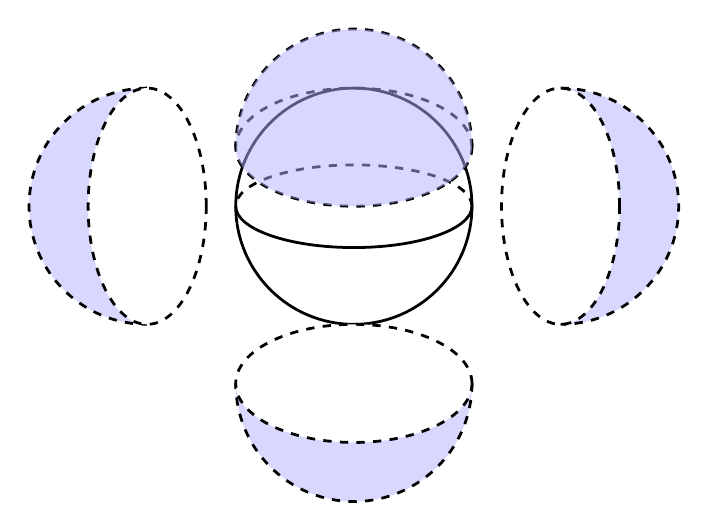
\begin{tikzpicture}[scale=1.5]
  \draw[line width=1, dashed] (1,0) arc (0:180:1 and 0.35);
  \draw[line width=1] (1,0) arc (0:180:1 and -0.35);
  \draw[line width=1](0,0) circle (1);

  % Left Chart
  \path[fill=blue!30!white,opacity=0.5] (-1.75,1) arc (90:-90:-1 and 1);
  \draw[line width=1, dashed] (-1.75,1) arc (90:-90:-1 and 1);
  \draw[fill=white, line width=1, dashed] (-1.75,0) ellipse (0.5 and 1);

  % Right Chart
  \path[fill=blue!30!white,opacity=0.5,line width=1, dashed] (1.75,1) arc (90:-90:1 and 1);
  \draw[fill=white, line width=1, dashed] (1.75,0) ellipse (0.5 and 1);
  \draw[line width=1, dashed] (1.75,1) arc (90:-90:1 and 1);

  % Top Chart
  \draw[line width=1, dashed] (0,0.5) ellipse (1 and 0.5);
  \draw[line width=1, dashed] (1,0.5) arc (0:180:1 and 1);
  \path[fill=blue!30!white,opacity=0.5] (1,0.5) arc (0:-180:1 and 0.5);
  \path[fill=blue!30!white,opacity=0.5] (1,0.5) arc (0:180:1 and 1);


  % Bottom Chart
  \path[fill=blue!30!white,opacity=0.5,line width=1, dashed] (1,-1.5) arc (0:-180:1 and 1);
  \draw[line width=1, dashed] (1,-1.5) arc (0:-180:1 and 1);
  \draw[fill=white, line width=1, dashed] (0,-1.5) ellipse (1 and 0.5);
\end{tikzpicture}

			\caption{Representación de cuatro de las seis cartas suaves con las que cubrimos a la $2-$esfera.}
		\end{center}
	\end{figure}

	Si consideramos los conjuntos de cartas que $\{(U_i^{\pm}, \phi_{i}^{\pm})\}_{i=1}^{n}$ y las inversas de estas funciones se definen en el ejemplo \ref{Ex: Variedad Topologica - Esfera}. Para cualesquiera dos cartas se tendrán dos casos, los índices $i,j$ son iguales o son diferentes. En el caso en que los índices son iguales se tiene que el mapa de transición es:

	\[ \phi_i^{+} \circ \left(\phi_{i}^{-}\right)^{-1} = \phi_i^{-} \circ \left(\phi_{i}^{+}\right)^{-1} = \id_{\B^n} \]
	En el caso en el que los índices son diferentes tendremos que el mapa de transición está dado como:
	\[ \phi_i^{+} \circ \left(\phi_{j}^{-}\right)^{-1}(u_1, \dots, u_n) = \left(u_1, \dots, \underbrace{\pm \sqrt{1 - \|u\|^2}}_{j-\text{ésimo término}},\dots, u_{i-1}, u_{i+1}, \dots, u_{n} \right) \]

	En ambos casos las composiciones son diferenciables y en ningún punto cero, podemos concluir entonces que ambas son difeomorfismos. Por lo tanto, determinan una estructura suave en $\S^n$.
\end{example}

\begin{example}[Producto Finito de Variedades Suaves]\label{Ex: Variedad Suave - Producto de Variedades Suaves}
	Si $M_1^{n_1},\dots,M_k^{n_k}$ son variedades suaves entonces $M_1 \times \dots \times M_k$ es una variedad suave. Como se hizo en el ejemplo \ref{Ex: Variedad Topologica - Producto de Variedades} procederemos considerando el producto de únicamente dos variedades suaves, el caso para el producto de un número arbitrario pero finito se seguirá por inducción.
	En el ejemplo \ref{Ex: Variedad Topologica - Producto de Variedades} probamos que si $M_1$ y $M_2$ son variedades topológicas con cartas de $(U,\phi)$ y $(V,\psi)$ respectivamente entonces $M_1 \times M_2$ es una variedad topológica y tiene cartas de la forma $(U \times V,\phi \times \psi)$. Si $M_1$ y $M_2$ son variedades suaves y consideramos dos cartas cualesquiera $(U_1 \times V_1, \phi_1 \times \psi_1)$, $(U_2 \times V_2, \phi_2 \times \psi_2)$ de $M_1 \times M_2$ entonces tendremos que el mapa de transición será:
	\[
		(\phi_2 \times \psi_2) \circ (\phi_1 \times \psi_1)^{-1} = (\phi_2 \circ \phi_1^{-1}) \times (\psi_2 \circ \psi_1^{-1})
	\]
	Como $M_1$ y $M_2$ son variedades suaves las cartas $(U_1,\phi_1)$, $(U_2,\phi_2)$, $(V_1,\psi_1)$, $(V_2,\psi_2)$ serán suavemente compatibles. Por lo tanto $M_1 \times M_2$ es una variedad suave.
\end{example}

Es importante no perder de vista que una variedad topológica no es suave en sí misma, la suavidad es una estructura adicional que se le agrega a la variedad a través de la estructura suave. Como se mencionaba anteriormente para una misma variedad pueden existir muchos atlas y muchos de ellos pueden ser atlas suaves o atlas maximales.

Para los ejemplos anteriores se ha mostrado que estas son variedades suaves comenzando con un espacio topológico y luego mostrando que este cumple con la definición de variedad topológica y finalmente ser dotado de una estructura suave. El siguiente lema nos da una alternativa, dándonos una manera de dotar a un conjunto de una estructura topológica y  una estructura suave.

\begin{lemma}\label{Lemma: Lema de Cartas Suaves de una Variedad}
	Sea $M$ un conjunto, $\{U_\alpha\}$ una colección de subconjuntos de $M$ y $\{\phi_\alpha\}$ una colección de mapas donde $\phi_\alpha: U_\alpha \to \R^n$ tales que las siguientes propiedades se cumplen:

	\begin{enumerate}
		\item Para cada $\alpha$, $\phi_\alpha$ es una biyección entre $U_\alpha$ y un subconjunto abierto $\phi_\alpha(U) \subseteq \R^n$.
		\item Para cualesquiera $\alpha, \beta$, los conjuntos $\phi_{\alpha}(U_\alpha \cap U_\beta)$ y $\phi_{\beta}(U_\alpha \cap U_{\beta})$ son ambos abiertos en $\R^n$.
		\item Si $U_\alpha \cap U_\beta \neq \varnothing$, el mapa $\phi_{\beta} \circ \phi_{\alpha}^{-1}: \phi_{\alpha}(U_{\alpha} \cap U_{\beta}) \to \phi_{\beta}(U_{\alpha} \cap U_{\beta})$ es suave.
		\item Existe una cubierta numerable para $M$ formada por elementos de $\{U_\alpha\}$.
		\item Si $p,q \in M$ y $p \neq q$, entonces existe un subconjunto $U_\alpha$ que contiene a $p$ y $q$, o existen subconjuntos disjuntos $U_{\alpha}$ y $U_{\beta}$ tales que $p \in U_{\alpha}$ y $q \in U_{\beta}$.
	\end{enumerate}

	Entonces $M$ tiene una estructura suave única tal que cada $(U_{\alpha},\phi_{\alpha})$ es una carta suave.
\end{lemma}

\begin{proof}
	Comenzaremos definiendo un conjunto el cual probaremos será una base para una topología en $M$. Sea $\mathcal{B}$ el conjunto formado por todos los $\phi_{\alpha}^{-1}(V) \in M$ tales que $V \subseteq \R^n$ es abierto. Por la propiedad 4 se garantiza que una subcolección numerable de $\mathcal{B}$ cubre a $M$, tomemos dos elementos de $\mathcal{B}$, $\phi_{\alpha}^{-1}(V)$ y $\phi_{\beta}^{-1}(W)$ y notemos que las siguientes igualdades se cumplen:
	\begin{align*}
		\phi_{\alpha}^{-1}(V) \cap \phi_{\beta}^{-1}(W) & = \phi_{\alpha}^{-1}(V) \cap (\phi_{\alpha}^{-1} \circ \phi_{\alpha} \circ \phi_{\beta}^{-1})(W)  \\
		                                                & = \phi_{\alpha}^{-1}(V) \cap \phi_{\alpha}^{-1} ((\phi_{\beta} \circ \phi_{\alpha}^{-1})^{-1}(W)) \\
		                                                & = \phi_{\alpha}^{-1} (V \cap (\phi_{\beta} \circ \phi_{\alpha}^{-1})^{-1}(W))
	\end{align*}

	Por la propiedad 3 sabemos que $\phi_{\beta} \circ \phi_{\alpha}^{-1}$ es suave, por lo que en particular será un mapa continuo, luego $(\phi_{\beta} \circ \phi_{\alpha})^{-1}(W)$ será abierto en $\R^n$, dado que será un subconjunto abierto de $\phi_{\alpha}(U_{\alpha} \cap U_{\beta})$ y este es, en sí mismo, un subconjunto abierto de $\R^n$ por la propiedad 2. Por lo propiedad 1 se garantiza que $\phi_{\alpha}^{-1}(V) \cap \phi_{\beta}(W) \in \mathcal{B}$, esto es suficiente para mostrar que $\mathcal{B}$ es una base para $M$.

	Ahora mostraremos que $M$ con la topología dada por la base $\mathcal{B}$ es, en efecto, una variedad topológica.

	Por definición de $\mathcal{B}$ cada $\phi_{\alpha}$ es un homeomorfismo sobre un subconjunto abierto de $\R^n$, por lo tanto, para cada $p \in M$ existirá una vecindad que lo contenga y un homeomorfismo de dicha vecindad sobre todo $\R^n$, esto prueba que $M$ con la topología dada es localmente euclidiano.

	Para mostrar que $M$ es Hausdorff con la topología consideremos $p, q \in M$ tales que $p \neq q$. Por la propiedad 5 solo existirán dos posibilidades, si existen subconjuntos $U_{\alpha}$, $U_{\beta}$ tales que $p \in U_{\alpha}$, $q \in U_{\beta}$ y $U_{\alpha} \cap U_{\beta} \neq \varnothing$ habremos terminado. La segunda posibilidad es que exista $U_{\alpha}$ tal que $p, q \in U_{\alpha}$, dado que $\phi_{\alpha}(U_{\alpha}) \subseteq \R^n$ es un subconjunto abierto existirán subconjuntos $V,W \subset \phi_{\alpha}(U_{\alpha})$ disjuntos tales que $\phi_{\alpha}(p) \in V$ y $\phi_{\alpha}(q) \in W$, por lo que $\phi_{\alpha}^{-1}(V)$ y $\phi_{\alpha}^{-1}$ serán vecindades disjuntas de $p$ y $q$. Por lo tanto $M$ con la topología dada es Hausdorff.

	La segundo numerabilidad de $M$ se tiene del hecho de que $\R^n$ es segundo numerable por lo que cada $\phi_{\alpha}(U_{\alpha})$ será segundo numerable, por ser $\phi_{\alpha}$ un homeomorfismo $U_{\alpha}$ será segundo numerable, y ocupando la propiedad 4 podemos concluir que $M$ es segundo numerable.

	Con esto hemos probado que $M$ es una variedad topológica. Y por la propiedad 3 podemos concluir que cada carta $(U_{\alpha},\phi_{\alpha})$ es una carta suave, por el teorema \ref{Teorema: Unicidad de Estructura Suave} se concluye que la estructura suave determinada por la colección de cartas es única.
\end{proof}

\cleardoublepage
\section{Mapas Suaves}\label{Sección: Mapas Suaves}
Habiendo definido las variedades topológicas y las variedades suaves ahora nos interesará estudiar lo que son los mapas suaves, estos son difeomorfismos entre variedades, los difeomorfismos son funciones o mapas bajo los cuales la estructura suave se preserva.

Haremos la siguiente distinción entre los términos \it{función} y \it{mapa}. Una mapa será una regla que a cada elemento de su dominio le asigna un elemento del contradominio, donde, el dominio y contradominio pueden ser variedades arbitrarias, mientras que una función será un tipo particular de mapa donde el contradominio es $\R^n$ para algún $n \in \N$.

\begin{definition}[Funciones Suaves]\label{Definición: Función Suave}
	Sea $M^n$ una variedad suave, $k$ un entero no negativo, y $f: M \to \R^{k}$ una función cualquiera. Diremos que $f$ es una \it{función suave} si para cada punto $p \in M$ existe una carta suave $(U,\phi)$ para $M$, cuyo dominio contiene a $p$ y tal que la composición de las funciones $f \circ \phi^{-1}$ es suave en el conjunto abierto $\phi(U) \subseteq \R^{n}$.
\end{definition}

\begin{figure}[h]
	\centering
	\begin{tikzpicture}[scale=0.85]
  \coordinate (a) at (0,0);
\path[draw,use Hobby shortcut,closed=true,thick]
(0,2.5) .. (2,2.5) .. (1,4.5) .. (.3,4.5) .. (-1,4) .. (-2,2.5);

\draw[dashed] (0.25,3.5) circle (0.6);
\draw node at (0,3.6) {$U$};
\draw node at (-1.5,4.5) {$M$};

\draw [thick, <->] (-5,0) -- (-1,0);
\draw [thick, <->] (-3,-2) -- (-3,2);
\draw [thick, <->] (1,0) -- (5,0);
\draw [thick, <->] (3,-2) -- (3,2);

\draw [dashed,thick] (-3,-0.25) ellipse  (1.5 and 1.2);


\draw[line width=1, ->] (1,3.75) arc (90:0:2.5);
\draw[line width=1, ->] (-0.75,3.5) arc (-90:0:-2);
\draw[line width=1, ->] (-1.5,-1.5) arc (60:120:-3.5);

\draw node at (-2.75,3) {$\phi$};
\draw node at (3.25,3) {$f$};
\draw node at (-2.25,-0.5) {$\phi(U)$};
\draw node at (-4.5,1) {$\R^n$};
\draw node at (4.5,1) {$\R^{k}$};
\draw node at (0.5,-1.25) {$f \circ \phi^{-1}$};
\end{tikzpicture}

	\caption{Representación de una función suave.}
\end{figure}

Notemos que en el caso en que la variedad que consideramos es $M = \R^n$ o algún subconjunto abierto de $\R^n$, la definición anterior coincide con la definición de cálculo multivariable ya que, como se vio en el ejemplo \ref{Ex: Variedad Suave - Espacios Euclidianos}, $\R^n$ es una variedad suave con la estructura suave dada por $(\R^n,\id_{\R^n})$ y al componer cualquier función con la identidad obtendremos la misma función.

Uno de los casos más importantes de las funciones suaves son aquellas que van de la variedad a los números reales, esto es, funciones suaves $f: M \to \R$. Al conjunto formado por estas funciones se le denota por $C^{\infty}(M)$, este es un espacio vectorial dado que la suma de funciones suaves y el producto de un escalar por una función suave son funciones suaves.

Podemos generalizar todavía más la noción de función suave si en lugar de restringirnos a $\R^k$ como el contradominio de las funciones dejamos que el contradominio sea cualquier variedad, esto se logra de la siguiente manera.

\begin{definition}[Mapa Suave]\label{Definición: Mapa Suave}
	Sean $M^{k_1}$ y $N^{k_2}$ variedades suaves, y sea $f: M \to N$ un mapa cualquiera. Diremos que $f$ es un \it{mapa suave} si para cada $p \in M$ existen cartas $(U,\phi)$ para $M$ cuyo dominio contiene a $p$ y $(V,\psi)$ para $N$ cuyo dominio contiene a $f(p)$ y $f(U) \subseteq V$, y tal que la composición $\psi \circ f \circ \phi^{-1}: \phi(U) \to \psi(V)$ es una función suave. A la composición $\psi \circ f \circ \phi{-1}$ se le llama la \it{representación coordenada de} $f$ con respecto a las coordenadas dadas.
\end{definition}

\begin{figure}[h]
	\centering
	\scalebox{.80}{\begin{tikzpicture}[scale=1]

%Variedad M
\path[draw,use Hobby shortcut,closed=true]
(-5,5.5) .. (-6,4) .. (-4,4) .. (-2,3.5) .. (-2.5,6);
\filldraw (-3,5) circle (0.05);
\node at (-3.25,5.25) {$p$};
\node at (-2.25,4.35) {$U$};
\draw[dashed] (-3,5) ellipse (0.6 and 0.8);
\node at (-1.25,5.75) {$M$};

%Variedad N
\path[draw,use Hobby shortcut,closed=true]
(5.5,6) .. (6,4) .. (4,3) .. (2,3.5) .. (2.5,5) .. (3.5,5.5);
\filldraw (3.25,4) circle (0.05);
\node at (2.75,3.6) {$F(p)$};
\node at (4.25,5) {$V$};
\draw[dashed](3.25,4) ellipse (1.2 and 0.9);
\node at (2,5.25) {$N$};

% Flecha M a N
\draw[thick,->] (-1,6) arc (-60:-130:-2.5);
\node at (0.25,6.75) {$F$};

% Flecha M a Rm
\draw[thick,->] (-3,4) arc (-10:20:-5);
\node at (-3.5,2.75) {$\phi$};

% Flecha N a Rn
\draw[thick,->] (3.75,3.25) arc (10:-20:4);
\node at (4.25,2) {$\psi$};

%Eje Izquierdo
\draw [<->] (-5,-1) -- (-1,-1);
\draw [<->] (-4,-1.5) -- (-4,2.5);
\node at (-5,2.5) {$\R^m$};
\node at (-1,1.25) {$\phi(U)$};
\draw[dashed] (-2.5, 0.25) circle (1);

%Eje Derecho
\draw [<->] (5,-1) -- (1,-1);
\draw [<->] (2,-1.5) -- (2,2.5);
\node at (1,2.5) {$\R^n$};
\node at (4.5,0) {$\psi(V)$};
\draw[dashed] (2.5, -0.25) circle (1.2);

% Flecha Rn a Rm
\draw[thick,->] (-2,-1.25) arc (60:120:-3.5);
\node at (0,-2) {$\psi \circ F \circ \psi^{-1}$};
\end{tikzpicture}
}
	\caption{Representación de un mapa suave.}
\end{figure}

Nuevamente lo que estamos haciendo es trasladar el problema, de modo que podamos determinar si un mapa es suave utilizando los conocimientos que ya tenemos de cálculo en varias variables.

A continuación mostraremos algunos resultados básicos sobre mapas suaves entre variedades, estos serán análogos a resultados de cálculo diferencial.

\begin{theorem}
	Todo mapa suave es continuo.
\end{theorem}

\begin{proof}
	Supongamos que $M$ y $N$ son variedades suaves y $f: M \to N$ es una mapa suave. Consideremos un punto arbitrario $p \in M$. Dado que $f$ es suave existirá un par de cartas $(U,\phi)$ y $(V,\psi)$ de $M$ y $N$ respectivamente, tales que:
	\[
		\psi \circ f \circ \phi^{-1}: \phi(U) \to \psi(V)
	\]
	es una función suave en el sentido usual, esto es, sus componentes tienen derivadas parciales de todos los órdenes, lo que implica que la composición $\psi \circ f \circ \phi^{-1}$ es continua. Por definición de carta $\phi$ y $\psi$ son homeomorfismos, por lo que al considerar la restricción:
	\[
		f |_{U} : \psi^{-1} \circ (\psi \circ f \circ \phi^{-1}) \circ \phi : U \to V
	\]
	esta será la composición de mapas continuos por lo que $f$ es continua en una vecindad de cada punto de $M$, por lo tanto, $f$ es continua.
\end{proof}

\begin{theorem}
	Sean $M$ y $N$ variedades suaves, y sea $f: M \to N$ un mapa suave.
	\begin{itemize}
		\item [a)] Si para cada $p \in M$ existe una vecindad $U$ tal que la restricción $f|_U$ es suave, entonces $f$ es suave.
		\item [b)] Si $f$ es suave, entonces su restricción a cada subconjunto abierto es suave.
	\end{itemize}
\end{theorem}

\begin{proof}
	\begin{itemize}
		\item[a)] Supongamos que para cada punto $p \in M$ existe una vecindad $U$ tal que $f|_U$ es un mapa suave. Por el ejemplo \ref{Ex: Variedad Suave - Subvariedades Suaves} sabemos que al ser $U$ un subconjunto abierto de $M$ también será una variedad suave, por lo que, por definición existirán cartas suaves $(\hat{U},\hat{\phi})$ de $U$ que contiene a $p$ y $(V,\psi)$ de $N$ que contiene a $f(p)$ y $f(\hat{U}) \subseteq N$ y tal que $\psi \circ f \circ \hat{\phi}^{-1}$ es un mapa suave. Dado que $\hat{U}$ es un abierto en $U$ con la topología de subespacio, $\hat{U}$ será abierto en $M$, por lo tanto $(\hat{U},\hat{\phi})$ es una carta en $M$ y $f$ es suave.

		\item [b)] Supongamos ahora que $f$ es suave. Sea $p \in M$ un punto arbitrario y $U$ es una vecindad abierta que lo contiene. Por definición de mapa suave existirán cartas $(\hat{U}, \phi)$ y $(V,\psi)$ cuyos dominios contienen a $p$ y $f(p)$ tales que $f(\hat{U}) \subset V$ y tal que $\psi \circ f \circ \phi^{-1}$ es un mapa suave. Tomando la carta $(U \cap \hat{U},\phi|_{U \cap \hat{U}} = \hat{\phi})$, esta es una carta de $U$ y cumple que $p \in U \cap \hat{U}$, $f(U \cap \hat{U}) \subseteq V$ y la composición $\psi \circ f \circ \hat{\phi}^{-1}$ es suave, podemos cubrir a $U$ con este tipo de cartas. Por lo tanto, la restricción de $f$ a cualquier subconjunto abierto es suave.
	\end{itemize}
\end{proof}

Este teorema lo que nos esta diciendo es que la suavidad es una propiedad local, también da pie al siguiente lema que nos permite construir mapas suaves.

\begin{corollary}[Lema de pegado para mapas suaves]
	Sean $M$ y $N$ variedades suaves, y sea $\{U_{\alpha}\}_{\alpha \in A}$ una cubierta abierta de $M$. Supongamos que para cada $\alpha \in A$ tenemos un mapa suave $f_{\alpha}: U_{\alpha} \to N$ tal que el mapa coincide en intersecciones, i.e., $f_{\alpha}|_{U_\alpha \cap U_\beta} = f_{\beta}|_{U_\alpha \cap U_\beta}$ para cualesquiera $\alpha$ y $\beta$. Entonces existirá un mapa único $f:M \to N$ tal que $f|_{U_\alpha} = f_{\alpha}$ para cada $\alpha \in A$.
\end{corollary}


\begin{theorem}\label{Teorema: Representación Suave}
	Sean $M$ y $N$ variedades suaves y $f: M \to N$ un mapa suave. Entonces la representación coordenada de $f$ con respecto a cualquier par de cartas suaves de $M$ y $N$ es suave.
\end{theorem}

\begin{proof}
	Consideremos dos cartas cualesquiera $(U,\phi)$ y $(V,\psi)$ de $M$ y $N$ respectivamente. Tenemos dos posibles casos:
	\begin{itemize}
		\item $U \cap f^{-1}(V) = \varnothing$, en este caso la proposición se cumple por vacuidad.
		\item $U \cap f^{-1}(V) \neq \varnothing$, en cuyo caso consideremos $p \in U \cap f^{-1}(V)$, de modo que $f(p) \in f(V)$. Dado que $f$ es suave existirán cartas $(\hat{U},\hat{\phi})$ y $(\hat{V},\hat{\psi})$ tal que $p \in \hat{U}$, $f(\hat{U})\subseteq \hat{V}$ y tales que $\hat{\psi} \circ f \circ \hat{\phi}^{-1}$. Como $M$ y $N$ son variedades suaves sus cartas serán suavemente compatibles por lo que $\hat{\phi} \circ \phi^{-1}: \phi(U \cap \hat{U}) \to \hat{\phi}(U \cap \hat{U})$ y $\psi \circ \hat{\psi}^{-1}: \hat{\psi}(V \cap \hat{V}) \to \psi(V \cap \hat{V})$ son suaves. Por lo tanto
		      \[
			      (\psi \circ \hat{\psi}^{-1}) \circ (\hat{\psi} \circ f \circ \hat{\phi}^{-1}) \circ (\hat{\phi} \circ \phi^{-1}) = \psi \circ f \circ \phi^{-1}: \phi(U \cap \hat{U} \cap f^{-1}(V)) \to \psi(V).
		      \]

		      Como el punto $p \in M$ era arbitrario se concluye que la representación coordenada de $f$ es suave en $\phi(U \cap f^{-1}(V))$
	\end{itemize}
\end{proof}


\begin{theorem}[Mapas Constantes]
	Sean $M^{n_1}$ y $N^{n_2}$ variedades suaves, cualquier mapa constante $c: M \to N$ es suave.
\end{theorem}

\begin{proof}
	En efecto, consideremos un punto arbitrario $p \in M$ y cartas $(U,\phi)$ y $(V,\psi)$ de $M$ y $N$ respectivamente que contengan a $p$ y $c(p)$. Claramente se tendrá que $c(p) = c(U) \subset V$ y además $\psi \circ c \circ \phi^{-1}: \phi(U) \to \psi(c(p))$, por lo que la representación coordenada de $c$ es una función constante de $\R^{n_1}$ a $\R^{n_2}$, por lo tanto será suave lo cual implica que $c$ es suave.
\end{proof}

\begin{theorem}[El Mapa Identidad]
	Sea $M^n$ una variedad suave, el mapa $\id: M \to M$ es suave.
\end{theorem}

\begin{proof}
	Sea $p \in M$ un punto arbitrario, podemos considerar una única carta $(U,\phi)$ que lo contenga, trivialmente tenemos que $\id(U) \subseteq U$, la representación coordenada de $\id$ está dada por $\phi \id \phi^{-1}: \phi(U) \to \phi(U)$, esta composición es suave dado que la función identidad es suave en $\R^n$, así, el mapa identidad es suave.
\end{proof}

\begin{theorem}[El Mapa De Inclusión]\label{Teorema: Mapa De Inclusion}
	Sea $M$ una variedad suave. Si $U \subseteq M$ es una subvariedad abierta, entonces el mapa de inclusión $\iota: U \to M$ es suave.
\end{theorem}

\begin{proof}
	Sea $p \in M$ y sea $(\hat{U},\phi)$ una carta de $U$ que contenga a $p$. $(\hat{U},\phi)$ será una carta también en $M$ y $\phi \circ \iota \circ \phi^{-1}: \phi(U) \to \phi(U)$ es la función identidad, que es suave, por lo tanto $\iota$ es un mapa suave.
\end{proof}

\begin{theorem}[Composición de Mapas Suaves]\label{Teorema: Composición de Mapas Suaves}
	Sean $M,N$ y $P$ variedades suaves. Si $f: M \to N$ y $g: N \to P$ son mapas suaves, entonces $g \circ f: M \to P$ es suave.
\end{theorem}

\begin{proof}
	Sea $p \in M$ un punto arbitrario. Por definición de suavidad existirán cartas $(V,\psi)$ y $(W,\omega)$ tales que $f(p) \in V$, $g(f(p)) \in W$ y $g(V) \subseteq W$, y tales que $\omega \circ g \circ \psi^{-1}: \psi(V) \to \omega(W)$.

	Dado que $f$ es suave, en particular será continua por lo que $f^{-1}(V)$ será un subconjunto abierto de $M$ que contiene a $p$, por lo que existirá una carta suave $(U,\phi)$ de M tal que $p \in M$ y $U \subseteq f^{-1}(V)$, por el teorema \ref{Teorema: Representación Suave} sabemos que $\psi \circ f \circ \phi^{-1}: \phi(U) \to \psi(V)$ es suave. Entonces $(g \circ f)(V) \subseteq g(V) \subseteq W$ y $\omega \circ (g \circ f) \circ \phi^{-1}$ es suave por ser la composición de mapas suaves entre espacios euclidianos.
\end{proof}

\begin{theorem}\label{Teorema: Mapa a Producto de Variedades Suaves}
	Sean $M_1,\dots,M_k$ y $N$ variedades suaves. Para cada $i$ sea $\pi_i: \prod_{i=1}^{k} M_i \to M_i$ la proyección sobre el factor $M_i$. Un mapa $f: N \to \prod_{i=1}^{k} M_i$ es suave si y sólo si cada uno de sus mapas componentes $f_i = \pi_i \circ f: N \to M_i$ es suave.
\end{theorem}

\begin{proof}
	Probaremos el caso para el producto de dos variedades, el caso general se sigue por inducción. Sean $M_1, M_2, N$ variedades suaves. Sean $\pi_1: M_1 \times M_2 \to M_1$ y $\pi_2: M_1 \times M_2 \to M_2$ las proyecciones. Procederemos por partes:

	\begin{itemize}
		\item Las proyecciones son suaves. Sin pérdida de generalidad consideremos la proyección sobre la primera coordenada.
		      Sean $p \in M_1^{n_1} \times M_2^{n_2}$ un punto arbitrario, $(U \times V,\phi \times \psi)$ una carta de $M_1 \times M_2$ que contiene a $p$, $(U, \omega)$ una carta de $M_1$ que contiene a $\pi_1(p)$, tenemos que $\pi(U \times V) \subseteq U$. Tenemos que:
		      \begin{align*}
			      \omega \circ \pi_1 \circ (\phi \times \psi)^{-1}(x,y) & =  \omega(\pi_1 (\phi^{-1}(x), \psi^{-1}(y))) \\
			                                                            & = \omega(\phi^{-1}(x))                        \\
			                                                            & = \omega \circ \phi^{-1}(x)
		      \end{align*}

		      Esto es una proyección de $\R^{n_1 + n_2}$ a $\R^{n_1}$ que sabemos es suave. Por lo tanto la proyección del producto de variedades suaves será suave en cada punto, esto implica que la proyección sobre una de las coordenadas es suave en todo el dominio.

		\item Sea $f: N \to M_1 \times M_2$ un mapa suave, por el teorema \ref{Teorema: Composición de Mapas Suaves} sabemos que las composiciones $\pi_1 \circ f$ y $\pi_2 \circ f$ son suave.

		\item Sean $\pi_1 \circ f$ y $\pi_2 \circ f$ mapas suaves. Sean $p \in N$, $(U,\phi)$ una carta de $N$ que contiene a $p$ y $(V,\psi)$, $(W,\omega)$ cartas de $M_1$ y $M_2$ respectivamente tales que $\pi_1 \circ f (U) \subseteq V$ y $\pi_2 \circ f(U) \subseteq W$ y tales que:
		      \begin{align*}
			      \psi \circ (\pi_1 \circ f) \circ \phi^{-1}   & : \phi(U) \to \psi(V)   \\
			      \omega \circ (\pi_2 \circ f) \circ \phi^{-1} & : \phi(U) \to \omega(W)
		      \end{align*}

		      Son cartas suaves. Tendremos que $(V \times W, \psi \times \omega)$ es una carta para $M_1 \times M_2$ tal que $f(U) \subseteq V \times W$, y su representación coordenada será:
		      \[
			      (\psi \times \omega) \circ f \circ \phi^{-1}: \phi(U) \to \psi(V) \times \omega(W)
		      \]

		      Esta composición es suave dado que sus proyecciones de $\R^{n_1} \times \R^{n_2}$ a cada una de sus componentes son suaves.
	\end{itemize}
\end{proof}

Un hecho importante sobre el conjunto de funciones suaves, $C^{\infty}(M)$, es que este es un anillo bajo la suma y el producto, por lo cual bajo dichas operaciones el conjunto tiene propiedades algebraicas muy agradables, similares a las de un campo, recordemos que la definición de anillo es la siguiente.

\begin{definition}[Anillo]
	Un \it{anillo} es un conjunto $\K$ junto con dos operaciones $(x,y) \to x + y$ y $(x,y) \to xy$, las cuales satisfacen las siguientes propiedades:
	\begin{itemize}
		\item $\K$ es un grupo conmutativo bajo la operación $(x,y) \to x + y$
		\item $(xy)z = x(yz)$
		\item $x(y + z) = xy + xz$ y $(y+z)x = yx + yz$
	\end{itemize}
\end{definition}

Si ademas se tiene que $xy = yx$ para cada $x,y \in \K$ diremos que $\K$ es un \it{anillo conmutativo} y, si existe un elemento $1 \in \K$ tal que $1x = x1 = x$ para cada $x \in \K$ entonces diremos que $\K$ es un \it{anillo con identidad}.

Para probar que, en efecto, el conjunto de funciones suaves $C^{\infty}(M)$ es un anillo haremos uso del siguiente lema.

\begin{lemma}
	Si $M$ es una variedad suave y $f: M \to \R^{k}$ es una función suave, entonces para cada carta suave $(U,\phi)$ se tiene que la composición $f \circ \phi^{-1}: \phi(U) \to \R^{k}$ es una función suave.
\end{lemma}

\begin{proof}
  Tomemos un $p \in M$ arbitrario y una carta $(U, \phi)$ que lo contenga. Por definición de función suave existirá un carta $(V,\psi)$ tal que la composición $f \circ \psi^{-1}: \psi(V) \to \R^{k}$ es suave.

  Al ser $(U,\phi)$ y $(V,\psi)$ cartas suaves, el mapa de transición $\psi \circ \phi^{-1}: \phi(U \cap v) \to \psi(U \cap V)$ es suave, por lo que $(f \circ \psi^{-1}) \circ (\psi \circ \phi^{-1}) = f \circ \phi^{-1}: \phi(U \cap V) \to \R^{k}$ es un mapa suave. Como $p$ es un punto arbitrario podemos concluir que esto cumplirá para cada punto de $U$, por lo cual $f \circ \phi^{-1}$ es suave en $\phi(U)$, para cada carta suave$(U,\phi)$.
\end{proof}

\begin{theorem}
	El conjunto de funciones suaves, $C^{\infty}(M)$, es un anillo conmutativo con identidad bajo las operaciones:
	\begin{alignat*}{2}
		(f+g)(p) & = f(p) + g(p), \quad & p \in M               \\
		(fg)(p)  & = f(p)g(p),          & f,g \in C^{\infty}(M)
	\end{alignat*}
\end{theorem}

\begin{proof}
  Consideremos dos funciones $f,g \in C^{\infty}(M)$, mostraremos que tanto la suma como el producto de estas funciones son suaves.

  Por el lema anterior sabemos que para cualquier carta suave $(U,\phi)$, las composiciones $f \circ \phi^{-1}$ y $g \circ \phi^{-1}$ son suaves y, por como definimos la suma tenemos que $(f + g)\circ \phi^{-1} = (f \circ \phi^{-1}) + (g \circ \phi^{-1})$, esta la suma de funciones suaves en el sentido usual, la cual sabemos es suave.

  De modo similar para el producto se tendrá por definición que, $(fg)\circ\phi^{-1} = (f \circ \phi^{-1}) (g \circ \phi^{-1})$ y por el mismo motivo, por ser el producto de funciones suaves en el sentido usual, el producto $(fg) \circ \phi^{-1}$ es suave.

  La conmutatividad, la asociatividad y la distributividad se tendrán del hecho que la suma y el producto cumplen estas propiedades se cumplen en $\R$, y como hemos visto anteriormente, las constantes también son mapa suaves, por lo que la unidad será la identidad.
\end{proof}

\subsection{Difeomorfismos}\label{Subsección: Difeomorfismos}
Ahora estudiaremos un tipo particular de mapa suave, los difeomorfismos. De modo similar a como los homeomorfismos preservan ciertas propiedades de los espacios topológicos, los difeomorfismos entre variedades suaves preservarán ciertas propiedades de la estructura suave.

\begin{definition}[Difeomorfismo]\label{Definición: Difeomorfismo}
  Sean $M$ y $N$ variedades suaves y $f: M \to N$ un mapa cualquiera. Diremos que $f$ es un \it{difeomorfismo} si:
\begin{itemize}
  \item $f$ es un homeomorfismo.
  \item $f: M \to N$ es un mapa suave.
  \item $f^{-1}: N \to M$ es un mapa suave.
\end{itemize}
\end{definition}

\begin{theorem}\label{Teorema: Composición de Difeomorfismos}
Sean $M, N$ y $P$ variedades suaves, $f: M \to N$ y $g: N \to P$ difeomorfismos. La composición $g \circ f: M \to P$ es un difeomorfismo.
\end{theorem}

\begin{proof}
\begin{itemize}
\item La composición $g \circ f$ es un homeomorfismo por ser la composición de homeomorfismos.
\item Dado que $f$ y $g$ son mapas suaves, por el teorema \ref{Teorema: Composición de Mapas Suaves} sabemos que la composición $g \circ f$ es un mapa suave.
\item Por ser $f$ y $g$ difeomorfismos, $f^{-1}$ y $g^{-1}$ también son mapas suaves, nuevamente tenemos que por el teorema \ref{Teorema: Composición de Mapas Suaves} el mapa $(g\circ f)^{-1} = f^{-1} \circ g^{-1}$ es suave.
\end{itemize}
\end{proof}

\begin{theorem}
  Sean $M_1, \ldots, M_k$ y $N_1, \ldots N_k$ variedades suaves, y sean $f_i: M_i \to N_i$ difeomorfismos, el producto cartesiano de mapas $f_1 \times \cdots \times f_k : M_1 \times \cdots \times M_k \to N_1 \times \cdots \times N_k$ definido como:
  \[
    (f_1 \times \cdots \times f_k)(x_1, \ldots, x_k)
    = 
    (f_1(x_1), \ldots, f(x_k)), 
  \]
  es un difeomorfismo.
\end{theorem}

\begin{proof}
  Probaremos el caso para el producto cartesiano de dos mapas. Sean $M_1, M_2$ y $N_1, N_2$ variedades suaves, y sean $f: M_1 \to N_1$ y $g: M_2 \to N_2$ difeomorfismos.

  Dado que el producto cartesiano de mapas continuos es continuo, $f \times g$ es un mapa continuo de $M_1 \times M_2$ a $N_1 \times N_2$, además, $f \times g$ es un mapa invertible, y su inversa está dada como el producto cartesiano de los mapas inversos a $f$ y $g$, esto es,
  \[
    (f \times g)^{-1} = f^{-1} \times g^{-1}
  \]
  Y dado que $f$ y $g$ son difeomorfismos, en particular serán homeomorfismos, por lo cual sus inversas serán continuas, así podemos garantizar que $(f \times g)^{-1}$ es un mapa continuo y $f \times g$ es un homeomorfismo.


  Por el teorema \ref{Teorema: Mapa a Producto de Variedades Suaves} sabemos que el producto $f \times g$ es un mapa suave si y solo si cada una de sus componentes es suave, pero esto se tiene por hipótesis, dado que tanto $f$ como $g$ son suaves, y al tomar las proyecciones del producto cartesiano sobre sus mapas componentes obtenemos:
  \begin{align*}
    \pi_1 \circ (f \times g) &= f \\
    \pi_2 \circ (f \times g) &= g
  \end{align*}

  Del mismo modo podemos tomar las proyecciones del mapa $(f \times g)^{-1}$ y ver que estas proyecciones son suaves. Por lo tanto, el producto cartesiano de dos difeomorfismos es un difeomorfismo. El caso general se tiene por inducción.
\end{proof}

\begin{theorem}
  Sean $M$ y $N$ variedades suaves, $U \subseteq M$ una subvariedad abierta y $f: M \to N$ un difeomorfismo. La restricción $f|_{U}: U \to f(U) \subseteq N$ es un difeomorfismo.
\end{theorem}

\begin{proof}
  La restricción de un homeomorfismo a un subconjunto abierto es nuevamente un homeomorfismo. Además, podemos expresar la restricción de una función a un conjunto como $f|_U = f \circ \iota$, donde $\iota: U \to M$ es el mapa de inclusión, como se demostró en el teorema \ref{Teorema: Mapa De Inclusion} este es suave, por lo tanto, la composición será suave, lo que implica que $f|_U$ es suave.

  Dado que $f$ es un homeomorfismo y $U$ es abierto se garantiza que $f(U)$ es un subconjunto abierto, y por el argumento anterior podemos concluir que $(f|_U)^{-1}$ es un mapa suave.
\end{proof}

Estas son algunas propiedades básicas de los difeomorfismos, a continuación, veremos dos resultados que nos dicen que si tenemos un difeomorfismo entre dos variedades suaves estas son esencialmente la misma.

\begin{theorem}
  El conjunto de todas las variedades difeomorfas forma una clase de equivalencias. 
\end{theorem}

\begin{proof} Sean $M,N$ y $P$ variedades suaves, y sean $f: M \to N$ y $g: N \to P$ difeomorfismo, entonces:
  \begin{itemize}
    \item $M \sim M$. La identidad $\id: M \to M$ es un difeomorfismo de una variedad consigo misma, esto se tiene trivialmente.
    \item $M \sim N$ implica $N \sim M$. Si $f: M \to N$ es un difeomorfismo entonces su inversa, $f^{-1}: N \to M$ también es un difeomorfismo.
    \item Si $M \sim N$ y $N \sim P$, entonces $M \sim P$. Por el teorema \ref{Teorema: Composición de Difeomorfismos} sabemos que la composición de difeomorfismos es un difeomorfismo.
  \end{itemize}
\end{proof}

\begin{theorem}[Invariancia de la Dimensión]
  Si $M^m$ y $N^n$ son variedades suaves no vacías no puede existir un difeomorfismo de $M$ a $N$, a menos que $m=n$
\end{theorem}

\begin{proof}
  Para probar este teorema primero probaremos un resultado similar en espacios euclidianos. Sean $\R^n$ y $\R^m$ espacios euclidianos y $f: \R^n \to \R^n$ un difeomorfismo, entonces $m = n$.

  Por ser un $f: \R^n \to \R^m$ difeomorfismo su función inversa  $f^{-1}: \R^m \to \R^n$ existirá. Por definición de función invertible tenemos que $f^{-1} \circ f (x) = x$ y $f \circ f^{-1}(y) = y$, por la regla de la cadena tenemos que:
  \begin{align*}
    D(f^{-1} \circ f)(x) &= Df^{-1}(f(x))Df(x) = \id_{\R^n}\\
    D(f \circ f^{-1})(y) &= Df(f^{-1}(y))Df^{-1}(x) = \id_{\R^m}
  \end{align*}

  Donde $D$ representa la derivada total. De aquí podemos concluir que la matriz de la derivada total es invertible, y por un resultado básico de álgebra lineal tenemos que la matriz debe ser cuadrada, por lo tanto, $m = n$.

  Ahora, si $p \in M$ es un punto arbitrario, $(U,\phi)$ y $(V,\psi)$ son cartas suaves que contienen a $p$ y $f(p)$ respectivamente, entonces la representación coordenada $\psi \circ f \circ \phi^{-1}: \R^m \to \R^n$ es un difeomorfismo. 
\end{proof}

\subsection{Funciones Características Suaves y Particiones de la Unidad} \label{Subsección: Funciones Características Suaves y Particiones De La Unidad}
Una herramienta que nos será de utilidad más adelantes son las particiones de la unidad, estas nos permiten extender funciones que estén definidas de manera local en una variedad suave de modo que estas sean suavemente cero fuera de sus dominios y de tal manera que podamos sumarlas obteniendo una función que esté definida globalmente.

\begin{definition}[Soporte De Una Función]\label{Definición: Soporte de una Función}
	Sea $M$ una variedad suave y $f: M \to \R^n$ una función suave. Definimos el \it{soporte de} $f$ como la cerradura del conjunto donde $f$ no sea anula, i.e.,

	\[ \sup f = \overline{ \{ p \in M : f(p) \neq 0 \}} \]

	Si $U \subseteq M$ y $\sup f \subseteq U$ diremos que $f$ \it{está soportada} o \it{tiene soporte en} $U$, y, si $\sup f$ es un conjunto compacto diremos que $f$ tiene \it{soporte compacto}.
\end{definition}

\begin{definition}[Función Indicadora Suave]\label{Definición: Función Indicadora Suave}
	Sea $M$ una variedad suave, $p \in M$ un punto arbitrario y $U$ una vecindad de $p$. Diremos que $f$ es una \it{función indicadora suave en $p$ con soporte en} $U$ si $f$ es una función suave con soporte en $U$ y $f$ es igual a $1$ en una vecindad de $p$.
\end{definition}


En el siguiente ejemplo construiremos una función indicadora suave.

\begin{example}\label{Ex: Función Indicadora}
	Consideremos la función por partes $f: \R \to \R$:
	\[ f(t) =
		\begin{cases}
			e^{-\frac{1}{t}} & t > 0    \\
			0                & t \leq 0
		\end{cases}
		\qquad \qquad
		\begin{gathered}
			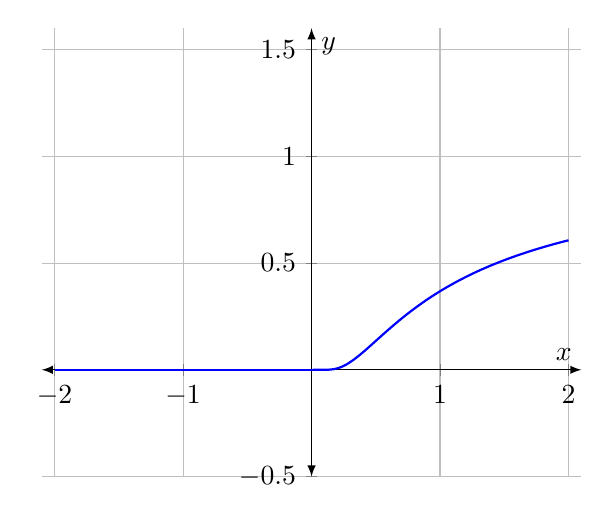
\begin{tikzpicture}
\begin{axis}[
  grid=both,
  xmin=-2.1,
  xmax=2.1,
  ymin=-0.5,
  ymax=1.6,
  axis lines=middle,
  xlabel = $x$,
  ylabel = $y$,
  axis line style={latex-latex},
  ]

\addplot[
  samples=100,
  domain=0.01:2,
  color=blue,
  thick,
  smooth,
  ]
  {(e)^(-1/x)};


\addplot[
  samples=2,
  domain=-2:0.01,
  color=blue,
  thick,
  smooth
  ]
  {0};

\end{axis}
\end{tikzpicture}

		\end{gathered}
	\]

	Comenzaremos mostrando que esta función es suave, procederemos en dos pasos:

	\begin{enumerate}
		\item La función es continua. Esto se tiene trivialmente calculando los límites laterales del cociente de Newton:
		      \begin{align*}
			      \lim_{t \to 0^+} \frac{f(t) - f(0)}{t} & = \lim_{t \to 0^+} \frac{e^{-\frac{1}{t}}}{t} = 0 \\
			      \lim_{t \to 0^-} \frac{f(t) - f(0)}{t} & = 0
		      \end{align*}
		\item Si $t > 0$, entonces la derivada $f^{(k)}$ tiene la forma $f^{(k)}(t) = p_k(t)\frac{e^{-\frac{1}{t}}}{t^{2k}}$ para algún polinomio $p_k$ con grado a lo más $k$.

		      Para $k = 0$ esto se cumplirá por definición de $f$. Supongamos que la propiedad se cumple para algún $k \geq 0$. Mostraremos que se cumple también para $f^{(k+1)}$:
		      \begin{align*}
			      f^{(k+1)}(t) & = \frac{d}{dt} f^{(k)}(t) = \frac{d}{dt} p_k(t) \frac{e^{-\frac{1}{t}}}{t^{2k}}                                                          \\
			                   & = p'_k(t) \frac{e^{-\frac{1}{t}}}{t^{2k}} + p_k(t) \frac{t^{-2} e^{-\frac{1}{t}}}{t^{2k}} - 2kp_k(t) \frac{e^{-\frac{1}{t}}}{t^{2(k+1)}} \\
			                   & = \left(t^2p'_k(t) + p_k(t) - 2ktp_k(t) \right) \frac{e^{-\frac{1}{t}}}{t^{2(k+1)}}
		      \end{align*}

		\item Claramente cuando tomamos los límite $\lim_{t \to 0^+} f^{(k)}(t)$ y $\lim_{t \to 0^-} f^{(k)}(t)$ ambos son cero.
	\end{enumerate}

	Por lo tanto $f$ es una función suave en todo $\R$

	Ahora, lo que queremos es utilizar la función $f$ para definir una función indicadora suave, el primer paso para poder lograr esto es definir la función $g: \R \to \R$ del siguiente modo:
	\[
		g(t) = \frac{f(t)}{f(t)+f(1-t)}
		\qquad \qquad
		\begin{gathered}
			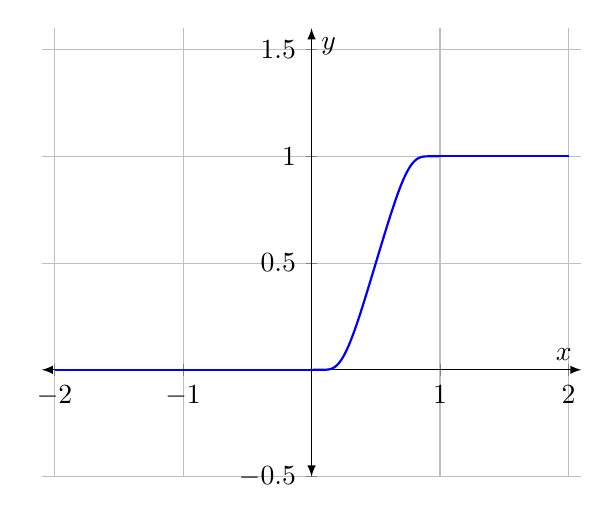
\begin{tikzpicture}
\begin{axis}[
  grid=both,
  xmin=-2.1,
  xmax=2.1,
  ymin=-0.5,
  ymax=1.6,
  axis lines=middle,
  xlabel = $x$,
  ylabel = $y$,
  axis line style={latex-latex},
  ]

\addplot[
  samples=100,
  domain=0.01:0.99,
  color=blue,
  thick,
  smooth,
  ]
  {((e)^(-1/x)) / ( ( e^(-1/x) ) + (e^(-1/(1-x))) )};


\addplot[
  samples=2,
  domain=-2:0.01,
  color=blue,
  thick,
  smooth
  ]
  {0};

\addplot[
  samples=2,
  domain=0.99:2,
  color=blue,
  thick,
  smooth
  ]
  {1};
\end{axis}
\end{tikzpicture}

		\end{gathered}
	\]


	Al ser $g$ el cociente de dos funciones suaves, y dado que el denominador no se anula en ningún punto, $g$ estará bien definida en todo $\R$ y además será suave. Lo que esta función $g$ nos da es una transición suave del $0$ al $1$, por lo cual, será sencillo construir una función indicadora suave a partir de esta, esto se logrará aplicando transformaciones sencillas.

	Si tomamos $a,b \in \R$ tales que $a<b$, podemos hacer un cambio de variables del conjunto compacto $[a^2,b^2]$ al conjunto $[0,1]$ del siguiente modo:

	\[
		x \mapsto \frac{x - a^2}{b^2 - a^2}
	\]

	Esta transformación nos permite cambiar la escala de $g$  y trasladarla en el eje horizontal,es por esta razón que se define $h: \R \to \R$ del siguiente modo,
	\[
		h(x) = g\left(\frac{x - a^2}{b^2 - a^2}\right)
		\qquad \qquad
		\begin{gathered}
			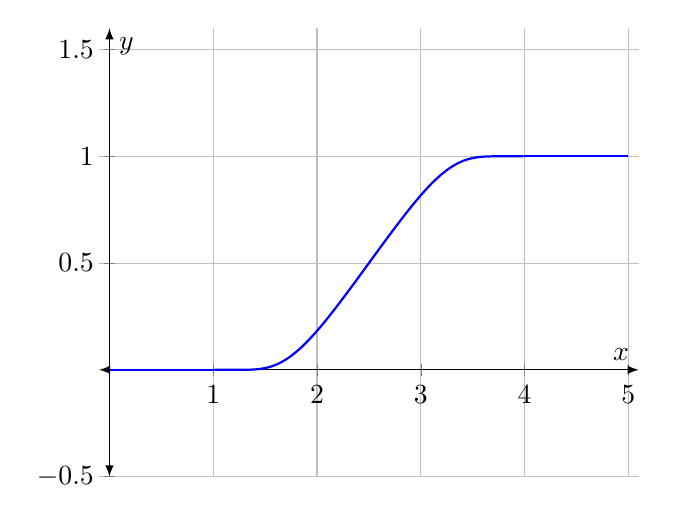
\begin{tikzpicture}
\begin{axis}[
  grid=both,
  xmin=-0.1,
  xmax=5.1,
  ymin=-0.5,
  ymax=1.6,
  axis lines=middle,
  xlabel = $x$,
  ylabel = $y$,
  axis line style={latex-latex},
  ]

\addplot[
  samples=100,
  domain=1.01:3.99,
  color=blue,
  thick,
  smooth,
  ]
  {((e)^(-1/ ((x - 1) / (4 - 1)) )) / ( ( e^(-1/ ((x - 1) / (4 - 1))) ) + (e^(-1/(1- ( (x - 1) / (4 - 1) )))) )};


\addplot[
  samples=2,
  domain=0:1.01,
  color=blue,
  thick,
  smooth
  ]
  {0};

\addplot[
  samples=2,
  domain=3.99:5,
  color=blue,
  thick,
  smooth
  ]
  {1};
\end{axis}
\end{tikzpicture}

		\end{gathered}
	\]

	Y de este modo al tomar $a,b \in \R$ como se acaba de hacer se tendrá que para $h$ se cumple lo siguiente

	\[
		h(x) = \begin{cases}
			1, & x > b^2    \\
			0, & x \leq a^2
		\end{cases}
	\]

	Ahora, podemos tomar $k(x)=h(x^2)$ para hacer que nuestra función sea simétrica alrededor del origen.

	\[
		k(x) = h(x^2) = g\left(\frac{x^2 - a^2}{b^2 - a^2}\right)
		\qquad \qquad
		\begin{gathered}
			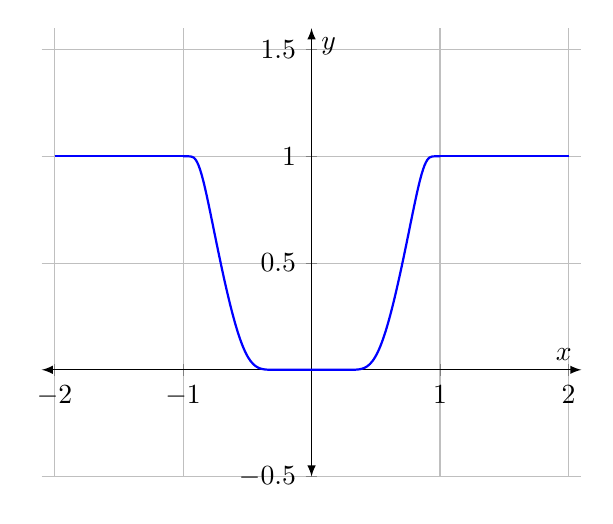
\begin{tikzpicture}
\begin{axis}[
  grid=both,
  xmin=-2.1,
  xmax=2.1,
  ymin=-0.5,
  ymax=1.6,
  axis lines=middle,
  xlabel = $x$,
  ylabel = $y$,
  axis line style={latex-latex},
  ]

\addplot[
  samples=100,
  domain=-1:1,
  color=blue,
  thick,
  smooth,
  ]
  {((e)^(-1/(x^2))) / ( ( e^(-1/(x^2)) ) + (e^(-1/(1-(x^2)))) )};


\addplot[
  samples=2,
  domain=-2:-0.99,
  color=blue,
  thick,
  smooth
  ]
  {1};

\addplot[
  samples=2,
  domain=0.99:2,
  color=blue,
  thick,
  smooth
  ]
  {1};
\end{axis}
\end{tikzpicture}

		\end{gathered}
	\]



	Y finalmente, definimos la función suave $r$ de modo que su valor sea $1$ en el intervalo y $0$ fuera de este haciendo un pequeño ajuste del siguiente modo.
	\[
		r(t) = 1 - k(x) = 1 - g\left(\frac{x^2 - a^2}{b^2 - a^2}\right)
		\qquad \qquad
		\begin{gathered}
			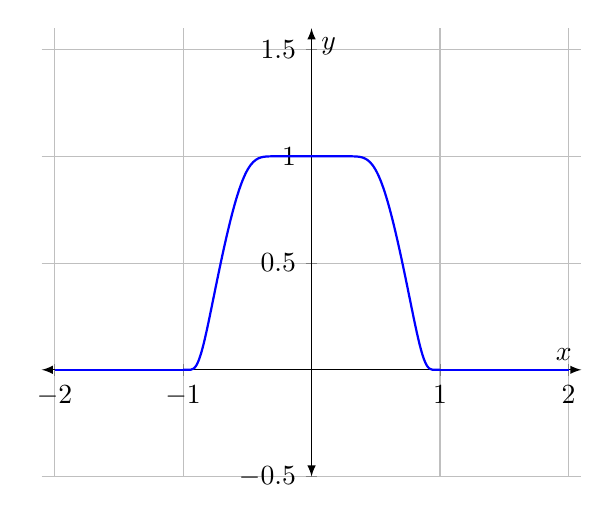
\begin{tikzpicture}
\begin{axis}[
  grid=both,
  xmin=-2.1,
  xmax=2.1,
  ymin=-0.5,
  ymax=1.6,
  axis lines=middle,
  xlabel = $x$,
  ylabel = $y$,
  axis line style={latex-latex},
  ]

\addplot[
  samples=100,
  domain=-1:1,
  color=blue,
  thick,
  smooth,
  ]
  {1 -( ((e)^(-1/(x^2))) / ( ( e^(-1/(x^2)) ) + (e^(-1/(1-(x^2)))) ))};


\addplot[
  samples=2,
  domain=-2:-0.99,
  color=blue,
  thick,
  smooth
  ]
  {0};

\addplot[
  samples=2,
  domain=0.99:2,
  color=blue,
  thick,
  smooth
  ]
  {0};
\end{axis}
\end{tikzpicture}

		\end{gathered}
	\]

	$r(t)$ es una función indicadora suave en $0$  y para cualquier $q \in \R$ tenemos que $r(x-q)$ es una función indicadora en $q$. Esta idea puede ser extendida a $\R^n$ como una función indicadora suave en $0 \in \R^n$  cuyo valor es $1$ en la bola (cerrada) $B_a(0)$ y $0$ fuera de la bola $B_b(0)$ si tomamos la función $r: \R^n \to \R$ cómo:

	\[
		\sigma(x) = r(\|x\|) = 1 - g\left(\frac{\|x\| - a^2}{b^2 - a^2}\right)
	\]
\end{example}

\begin{figure}
\centering
\begin{tikzpicture}[scale=1.25]
	\begin{axis}[
      view={30}{30},
			colormap/cool,
			xmin=-2,
			xmax=2.5,
			ymin=-2.5,
			ymax=2,
			zmin=-0.25,
			zmax=1.5,
			% axis lines=middle,
		]
		\addplot3[
			domain=-1.9:2.4,
			domain y = -2.4:1.9,
			patch,
			patch type=bilinear,
			shader=faceted interp,
		]
		{abs(x^2 + y^2) < 1 ? e^(-1 / (1 - abs(x^2 + y^2)) ) : 0 };

	\end{axis}
\end{tikzpicture}

\caption{Representación de una función indicadora suave en $\R^2$}
\end{figure}


Lo que haremos a continuación será extender estas ideas, mostraremos que para un cualquier punto en una variedad y cualquier vecindad que contenga a ese punto podemos encontrar una función indicadora suave en el punto con soporte en la vecindad.

\begin{lemma}\label{Lemma: Existencia de Función Indicadora}
	Sea $M^n$ una variedad suave, $p \in M$ un punto arbitrario y $U \subseteq M$ una vecindad de $p$. Entonces existe una función indicadora suave en $p$ con soporte en $U$.
\end{lemma}

\begin{proof}
	Sea $a$ un punto arbitrario en $M$ y $U$ una vecindad de $q$. Por ser $M$ una variedad suave existirá una carta suave $(V,\psi)$ que contiene a $q$ y tal que $V \subset U$.

	Consideremos la función $\sigma: \R^n \to \R$ definida anteriormente. $\sigma$ es una función indicadora suave en $\psi(q)$ con soporte en una bola compacta $B_r(\psi(q)) \subset V$. Definimos la función

	\[
		f(p) = \begin{cases}
			\sigma(\psi(p)), & p \in V    \\
			0,               & p \notin V
		\end{cases}
	\]

	Mostraremos que, en efecto, esta función es una función indicadora en $q$ con soporte en $U$.

	Por cómo hemos construido $\sigma$ esta tiene soporte compacto, esto es, $\sup \sigma$ es un conjunto compacto, luego $\psi^{-1}(\sup \sigma)$ será la imagen continua de un conjunto compacto, i.e., $\psi^{-1}(\sup \sigma)$ es un compacto en $M$. Dado que $M$ es Hausdorff podemos garantizar que $\psi^{-1} (\sup \sigma)$ es cerrado. Por lo tanto tendremos que
	\[
		\sup f \subset \phi^{-1} (\sup \sigma) \subset V
	\]

	Es claro que si $p \in V$, $f$ es suave en $p$ dado que $f(p)$ será la imagen de la composición de dos funciones suave. En el caso contrario, si $p \notin V$, entonces podremos elegir una carta $(W,\omega)$ que contengan a $p$ y tal que $W \cap \psi^{-1}(\sup \sigma) = \varnothing$. Entonce esta carta será también disjunta de $\sup f$, por lo que $f(W) \equiv 0$. Por lo tanto, $f$ será una función suave la cual es idénticamente $1$ en una vecindad de $V \subset U$ de $p$ y $\sup f \subset U$. Por lo tanto $f$ es una función indicadora suave en $q$ con soporte en $U$.
\end{proof}

\begin{lemma}
	Sea $M$ una variedad suave, $q$ un punto arbitrario, $U \subset M$ una vecindad de $q$ y $f$ una función indicadora suave en $q$ con soporte en $U$. Existe una función suave $\hat{f}$ en $M$ que coincide con $f$ en alguna vecindad, posiblemente más pequeña, que contiene a $q$.
\end{lemma}

\begin{proof}
	Si tomamos una función indicadora suave $r: \R^n \to \R$ cómo se construyó en el ejemplo \ref{Ex: Función Indicadora} de tal modo que $r$ tenga soporte en $U$ y esté definida en una vecindad $V$ de $q$, podemos definir la función:
	\[
		\hat{f} = \begin{cases}
			r(x)f(x), & x \in U    \\
			0,        & x \notin U
		\end{cases}
	\]

	Dado que $\hat{f}$ es el producto de funciones suaves en $U$, $\hat{f}$ es suave en $U$. Si $x \notin U$, entonces $x \notin \sup r$, por lo que existirá una vecindad que contiene a $x$ en la cual $\hat{f}$ se anula dado que, como se vio en el lema anterior, podemos tomar $\sup r$ cerrada. Por lo tanto $\hat{f}$ es suave en cada punto $x \notin U$. Y, dado que $r \equiv 1$ en $V$, la función $\hat{f}$ coincide con $f$ en $V$.
\end{proof}

Ahora utilizaremos algunos de los resultados que pueden ser encontrados en el Anexo \ref{Anexo: Topologia De Variedades} para poder dar las siguientes definiciones.

\begin{definition}[Partición de la Unidad Subordinada]\label{Definición: Partición de la Unidad Subordnada}
	Sea $M$ una variedad suave, y sea $\mathcal{U} = \{ U_\alpha \}_{\alpha \in A}$ una cubierta abierta de $M$. Una \it{partición de la unidad suave y subordinada a} $\mathcal{U}$ es una familia $\{ \phi_{\alpha} \}_{\alpha \in A}$ formada por funciones suaves y no negativas $\phi_{\alpha} : M \to \R$ tales que
	\begin{enumerate}
		\item $\sup \phi_\alpha \subseteq U_\alpha$, para cada $\alpha \in A$.
		\item La colección $\{\sup \phi_\alpha \}_{\alpha \in A}$ es localmente finita.
		\item $\sum_{\alpha \in A} \phi_\alpha (p) = 1$ para cada $p \in M$.
	\end{enumerate}
\end{definition}

Notemos que en el tercer punto de nuestra definición no tendremos problemas de convergencia dado que, por la segunda condición, al pedir que la colección de soportes de las funciones sea localmente finita, cada punto tendrá una vecindad $V$ que interceptará a $\{\sup \phi_{\alpha}\}_{\alpha \in A}$ en un subconjunto finito de $A$, por lo que la suma será finita.

\begin{theorem}[Existencia de Particiones Suave de la Unidad]\label{Teorema: Existencia de Particiones Suave de la Unidad}
	Sea $M$ una variedad suave y sea $\mathcal{U} = \{U_\alpha\}_{\alpha \in A}$ una cubierta abierta de $M$. Existe una partición suave de la unidad subordinada a $\mathcal{U}$.
\end{theorem}

\begin{proof}
	Por el resultado mostrado en el ejemplo \ref{Ex: Variedad Suave - Subvariedades Suaves}, $U_\alpha$ es en sí misma una subvariedad suave de $M$, y por los lemas \ref{Lemma: Bolas Precompactas} y \ref{Lemma: Base Por Bolas Suaves}, cada $U_\alpha$ tendrá una base $\mathcal{B}_\alpha$ formada por bolas coordinadas regulares y precompactas. Evidentemente $\mathcal{B} = \cup_{\alpha \in A} \mathcal{B}_\alpha$ formará una base para la topología de $M$.

	Por el teorema \ref{Teorema: Espacios Precompactos} y el corolario \ref{Corolario: Variedades Precompactas} podemos garantizar que $\mathcal{U}$ tendrá un refinamiento $\{B_i\}$ numerable y localmente finito que consta de elementos de $\mathcal{B}$.

	No es difícil ver que si $\{B_i\}$ es una colección localmente finita, entonces la colección formada por la cerradura de estos conjuntos $\{\overline{B}_i\}$ también será localmente finita.


	Dado que cada $B_i$ es una bola regular coordinada en algún $U_\alpha$, por definición existirá una bola coordinada suave $B_i' \subseteq U_\alpha$ tal que $\overline{B}_{i} \subseteq B_i'$, y un mapa suave $\phi_i: B_i \to \R^n$ tal que $\phi_i(\overline{B}_i) = \overline{B}_{r_i}(0)$ y $\phi_i(B_i') = B_{r_i'}(0)$ para algunos $r_i, r_i' \in \R$ tales que $r_i < r_i'$. Para cada $i$ definiremos la función $f_i: M \to R$ como:

	\[
		f_i(q)= \begin{cases}
			\rho_i \circ \phi_i, & p \in B_i'    \\
			0,                   & p \notin B_i'
		\end{cases}
	\]

	Como se mostró en el lema \ref{Lemma: Existencia de Función Indicadora} estas funciones son suaves, más aún, son funciones indicadoras suaves y además $\sup f_i = \overline{B}_i$.

	Con estas funciones podemos definir la función $f: M \to \R$ como $f(p) = \sum_i f_i(x)$. Dado que los $\{B_i\}$ y $\{\overline{B}_i\}$ son localmente finitos, la suma será finita y por lo tanto convergerá. Cómo cada $f_i$ es no negativa en cada punto en $B_i$, y cada punto de $M$ está en algún $B_i$ por ser la colección una cubierta de $M$, se sigue que $f(p) > 0$ para cada $p \in M$. Y por cómo hemos definido $\rho$ cada $f_i$ estará normalizada por lo que $0 \leq f_i \leq 1$ y $\sum_i f_i \equiv 1$.

	Por último hacemos un cambio de índices para nuestra funciones para que coincidan con los de la cubierta abierta $\mathcal{U}$. Dado que $\{B_i'\}$ es un refinamiento de $\mathcal{U}$, para cada $i$ podemos elegir algún índice $a(i) \in A$ tal que $B'_i \subseteq U_{a(i)}$. Para cada $\alpha \in A$ definimos la función $\psi_\alpha: M \to \R$ como:
	\[
		\psi_\alpha = \sum_{i : a(i) = \alpha} f_i
	\]

	Por estar cada $\psi_\alpha$ soportada en $\overline{B}_{i}$ tendremos que:
	\[
		\sup \psi_{\alpha} = \bigcup_{i: a(i)=\alpha} \subseteq U_\alpha
	\]

	Así, tendremos que la colección $\{\psi_{\alpha}\}$ es una partición de la unidad subordinada a $\mathcal{U}$.
\end{proof}

Los siguientes dos lemas nos darán maneras de extender funciones suaves utilizando particiones de la unidad, que en nuestro caso, es nuestro principal interés.

\begin{lemma}
	Sea $M$ una variedad suave, $p \in M$, $A \subset M$ un subconjunto arbitrario que contiene a $p$ y $f: A \to \R^{k}$ una función suave. Existe una extensión suave a un conjunto abierto que contiene a $A$, esto es, existe un conjunto abierto $U \subset M$ tal que $A \subset U$ y una función $\hat{f}: U \to \R^{k}$ tal que $\hat{f}|_{A \cap U} = f$.
\end{lemma}

\begin{proof}
	Consideremos una vecindad $V_p$ y una función suave $f_p: V_p \to \R^n$ para cada $p \in A$ tal que $f_{p}|_{V_p \cap A} = f|_{V_p \cap A}$. Por el teorema anterior podemos garantizar que existe una partición suave de la unidad $\{\psi_{p}\}_{p \in A}$ subordinada a $U=\cup_{p \in A}V_p$

	Definiremos el conjunto $B = \{p \in A: p \in \sup \psi_p\}$ y la función $\hat{f}: \cup_{p \in A} V_p \to \R^n$ como:
	\[
		\hat{f}(x) = \sum_{x \in B} \psi_p(x)f_p(x)
	\]

	$\hat{f}$ será una función suave que coincide con $f$ en el conjunto $U \cap A$, y por como se ha definido $U$, es claro que $A \subseteq U$.
\end{proof}

Notemos sin embargo que no siempre es posible extender una función suave a un conjunto más grande, en particular esto no siempre es posible si la función está definida en un conjunto abierto dado que el comportamiento de la función puede ser arbitrario. Como un ejemplo sencillo en $\R$ podemos tomar la función trigonométrica $\tan: (-\frac{\pi}{2}, \frac{\pi}{2}) \to \R$, para esta función no existe una extensión suave a un subconjunto abierto más grande.

Es por esto que damos el siguiente lema, el cual es un resultado más fuerte que el anterior, y nos garantiza que si imponemos la condición de que $A$ es cerrado, entonces podremos extender cualquier función suave definida en $A$ a cualquier subconjunto abierto que lo contenga a $A$.


\begin{lemma}[Lema de Extensión para Funciones Suaves]\label{Lemma: Lema de Extensión para Funciones Suaves}
	Sea $M$ una variedad suave, $A \subset M$ un subconjunto cerrado y $f: A \to \R^k$ una función suave. Para cada conjunto abierto $U$ que contiene a $A$ existe una función suave $\hat{f}: M \to \R^{k}$ tal que $\hat{f}|_{A} = f$ y $\sup(\hat{f}) = U$.
\end{lemma}

\begin{proof}
	Procederemos de modo similar a la demostración anterior. Para cada $p \in A$ tomemos una vecindad $V_p$ y una función suave $\hat{f}_p: V_p \to \R^k$ tal que $\hat{f}_p|_{V_p \cap A} = f$. Dado un conjunto abierto $U$ podemos reemplazar $V_p$ por $V_p \cap U$ y suponer que $V_p \subset U$.

	La colección de conjuntos $B=\{V_p: p \in A\} \cup (M - A)$ será una cubierta abierta para $M$, por el teorema \ref{Teorema: Existencia de Particiones Suave de la Unidad} podemos garantizar que existirá una partición suave de la unidad subordinada a la cubierta. Digamos que $\{\psi_p: p \in A\} \cup \{\psi_0 \}$ es dicha partición de tal modo que $\sup \psi_p \subseteq V_p$ y $\sup \psi_0 \subseteq M - A$.

	Definimos la función $\hat{f}: M \to \R^k$ como:
	\[
		\sum_{p \in A} \psi_p(x)\hat{f}_p(x)
	\]

	Esta suma es convergente y está formada por el producto de funciones suaves por lo que será suave, además coincide con $f$ en $U \cap A$ y tiene soporte en $U$ dado que será idénticamente cero fuera de $A$.
\end{proof}

\cleardoublepage

% ====================================
% Conceptos Básicos
% ====================================

\chapter{Título Pendiente}\label{Capítulo: Conceptos Básicos}
En este capítulo describiremos algunos conceptos básicos que eventualmente nos ayudarán a entender qué son las métricas, qué es una métrica Riemanniana y lo que son las variedades Riemannianas.

Los primeros conceptos que estudiaremos serán los espacios y fibrados tangentes. Existen varias definiciones equivalentes para lo que es un espacio tangente; nosotros procederemos a definirlo a partir de lo que llamaremos derivaciones, este enfoque tiene algunas ventajas algebraicas y se puede justificar con conceptos conocidos de cálculo multivariable. Comenzaremos contextualizando lo que queremos decir por espacio tangente en $\R^n$ y después generalizaremos la idea a variedades suaves.

Antes de comenzar necesitamos hacer la siguiente aclaración sobre la notación que utilizaremos, si consideramos un punto $p$ en $\R^n$ y queremos describir explícitamente sus coordenadas, esto lo haremos escribiendo entre paréntesis, $p = (p_1, \ldots, p_n)$; si en cambio consideramos un vector $v$ en $\R^n$, este puede ser representado por una matriz $n \times 1$, sin embargo, por conveniencia escribiremos $v = \begin{bmatrix} v_1 & \cdots & v_n \end{bmatrix}$, sin perder de vista que en realidad estamos hablando de la transpuesta de esta matriz.

\begin{definition}[Vectores y Espacios Tangentes en $\R^n$]\label{Definición: Espacio Tangente en Rn}
	Sea $a$ un punto en $\R^n$, definiremos el \it{espacio tangente a $\R^n$ en el punto $a$}, denotado por $T_a(\R^n)$, como el conjunto:
	\[ \{a\} \times \R^n = \{(a,v): v \in \R^n\} \]

	Un \it{vector tangente} a $\R^n$ es un elemento de $T_a(\R^n)$ para algún $a \in \R^n$. Denotaremos a un vector tangente $(a,v)$ particular como $v_a$ o $v|_a$ o simplemente $v$ para abreviar.
\end{definition}

En palabras más simples, lo que esta definición nos está diciendo es que el espacio tangente a $\R^n$ en algún punto $a$ es la colección de todos los vectores en $\R^n$ con origen en $a$.

Una de las propiedades más importantes del conjunto $T_a(\R^n)$ es que es un espacio vectorial bajo las operaciones

\[ v_a + w_a = (v + w)_{a}, \quad c(v)_{a} = (cv)_{a} \]

Por ser un espacio vectorial tendrá una base, no es difícil ver que si $\{e_i\}_{i=1}^n$ son los vectores de la base canónica para $\R^n$, entonces $\{e_i|_{a}\}_{i=1}^n = \{(a,e_i)\}_{i=1}^n$ será una base para $T_a(\R^n)$, al tener $n$ vectores básicos; llamamos a esta base la base estándar. $T_a(\R^n)$ será un espacio vectorial $n-$dimensional y por lo tanto será isomorfo a $\R^n$, de hecho $T_a(\R^n)$ es una copia de $\R^n$.

\begin{center}
\begin{figure}[h]
	\centering
	\begin{subfigure}{0.40\textwidth}
		\centering
    \begin{tikzpicture}
\draw[thick,->] (-0.5,0) -- (5,0) node[anchor=west]{$x$};
\draw[thick,->] (0,-0.5) -- (0,5) node[anchor=south]{$y$};

\draw (0.5,0.5) rectangle (4,4);
\node at (4.5,4.5) {$T_a(\R^n)$};

\draw[thick,->] (1,1.5) -- (3.5,1.5);
\draw[thick,->] (1.5,1) -- (1.5,3.5);
\filldraw (1.5,1.5) circle (0.1);
\node at (1,1) {$a$};
\draw[thick, ->] (1.5,1.5) -- (3,2.75);
  \node at (3.25,2.5) {$v_a$};
\end{tikzpicture}


	\end{subfigure}
	\begin{subfigure}{0.40\textwidth}
		\centering
    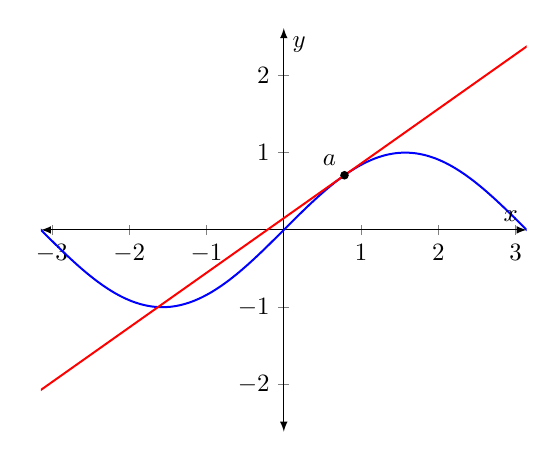
\begin{tikzpicture}[scale=0.90]
	\begin{axis}[
			% grid=both,
			xmin=-pi,
			xmax=pi,
			ymin=-1.6,
			ymax=1.6,
			axis lines=middle,
			xlabel = $x$,
			ylabel = $y$,
			axis line style={latex-latex},
      axis equal,
		]

		\addplot[
			samples=200,
			domain=-4*pi:4*pi,
			color=blue,
			thick,
			smooth,
		]
		{sin(deg(x))};

		\addplot[
			domain=-5:5,
			color=red,
      thick,
		]{( (sqrt(2) / 2) * (x - (pi/4)) ) +  (sqrt(2) / 2)};

		\addplot+[
			mark options={black},
      mark size=1.5pt,
		] coordinates {(0.785398,0.707106)} node [black, left=6pt, above=0.5pt] {$a$};
	\end{axis}
\end{tikzpicture}


	\end{subfigure}
  \\[20pt]
	\begin{subfigure}{0.40\textwidth}
		\centering
    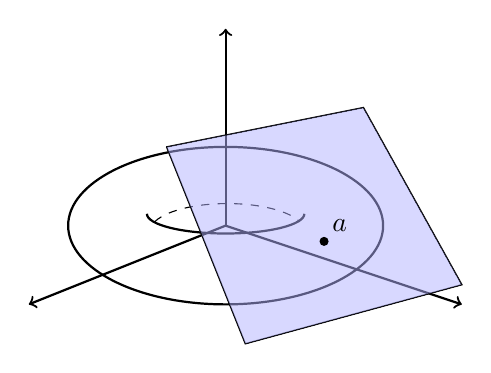
\begin{tikzpicture}

	% Ejes R3
	\draw [thick,->] (0,0) -- (0,2.5);
	\draw [thick,->] (0,0) -- (3,-1);
	\draw [thick,->] (0,0) -- (-2.5,-1);

	% Toro
	\draw [thick] (0,0) ellipse  (2 and 1);
	\draw [thick] (-1.0,0.15) arc (0:-180:-1.0 and 0.25);
  \draw [dashed] (-0.90,0.05) arc (20:160:-0.98 and 0.35);

  % Plano tangente
  \draw [line width=0.5] (-0.75,1) -- (1.75,1.5) -- (3,-0.75) -- (0.25,-1.5) -- (-0.75,1);
  \draw [fill=blue!30!white,opacity=0.5, line width=0] (-0.75,1) -- (1.75,1.5) -- (3,-0.75) -- (0.25,-1.5) -- (-0.75,1);

  % Punto $a$
	\filldraw (1.25,-0.2) circle (0.05);
	\node at (1.45,0) {$a$};
\end{tikzpicture}

	\end{subfigure}
	\begin{subfigure}{0.40\textwidth}
		\centering
    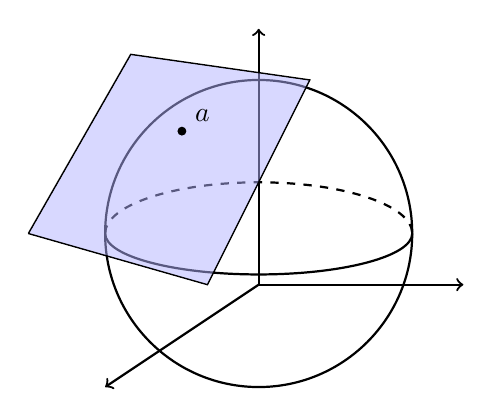
\begin{tikzpicture}[scale=0.65]
	% Esfera
	\draw [thick] (3,0) arc (0:180:3 and -0.8);
	\draw [thick, dashed] (-3,0) arc (180:0:3 and 1);
	\draw [thick] (0,0) circle (3);

	% Ejes R3
	\draw [thick,->] (0,-1) -- (0,4);
	\draw [thick,->] (0,-1) -- (4,-1);
	\draw [thick,->] (0,-1) -- (-3,-3);


	% Rectángulo (Espacio Tangente)
  \draw [fill=blue!30!white,opacity=0.5, line width=0] (-4.5,0) -- (-2.5,3.5) --(1,3.0) -- (-1,-1) -- (-4.5,0);
  \draw [line width=0.5] (-4.5,0) -- (-2.5,3.5) --(1,3.0) -- (-1,-1) -- (-4.5,0);
	\filldraw (-1.5,2) circle (0.075);
	\node at (-1.1,2.3) {$a$};
\end{tikzpicture}


	\end{subfigure}
\caption{Visualización de espacios tangentes a diferentes variedades.}
\end{figure}
\end{center}

Si en $\R^n$ consideramos un punto $a = (a_1, \dots, a_n)$ y un vector $v = \begin{bmatrix} v_1 \dots v_n \end{bmatrix}$, podemos dar la siguiente parametrización para la recta que pasa por $a$ con en la dirección de $v$:
\[ \gamma(t) = (a_1 + tv_1, \dots, a_n + tv_n) \]





\begin{definition}[Derivada Direccional]\label{Definción: Derivada Direccional}
	Sea $f: \R^n \to \R$ una función suave definida en una vecindad de un punto $a$ y $v \in T_a(\R^n)$, la \it{derivada direccional} de $f$ en $a$ en la dirección de $v$ se define como:
	\[ D_v f = \left. \frac{d}{dt} \right|_{t=0} f(\gamma(t)) \]
\end{definition}

Por la regla de la cadena podemos escribir la derivada direccional como:

\[D_v f = \sum_{i=1}^{n} \frac{d \gamma_i(0)}{dt} \frac{\partial f}{\partial x_i} (a)
	=\sum_{i=1}^n v_i \frac{\partial f}{\partial x_i} (a) \]

En este sentido, cada vector tangente $v_a \in T_a(\R^n)$ nos define un mapeo $D_v: C^{\infty}(\R^n) \to \R$ que nos da la derivada direccional de funciones suaves en un punto $a$ en la dirección de $v$. Dado que evaluamos la derivada direccional en el punto $a$, $D_v(f)$ será un número real.

Sabemos de cálculo que la derivada direccional es un operador lineal y además cumple la regla de Leibniz, esto es, si $f$ y $g$ son funciones suaves definidas en una vecindad de $a$, $c$ es una constante y $v$ es un vector tangente, entonces:

\begin{itemize}
	\item $D_v(cf) = c D_v(f)$.
	\item $D_v(f+g) = D_v(f) + D_v(g)$.
	\item $D_v(fg) = f(a) D_v(g) + g(a) D_v(f)$.
\end{itemize}

Basados en esta propiedad daremos la siguiente definición

\begin{definition}[Derivación en un punto]\label{Definición: Derivación en un punto de Rn}
	Sea $a$ un punto en $\R^n$ y $\omega: C^{\infty}(\R^n) \to \R$, diremos que $\omega$ es una \it{derivación en $a$} si es lineal y cumple la regla de Leibniz, i.e., si $f$ y $g$ son funciones suaves definidas en una vecindad de $a$, $c$ una constante

	\begin{itemize}
		\item $\omega(cf) = c \omega(f)$.
		\item $\omega(f+g) = \omega(f) + \omega(g)$.
		\item $\omega(fg) = f(a) \omega(g) + g(a) \omega(f)$.
	\end{itemize}

	Denotaremos al conjunto de todas las derivaciones de $C^{\infty}(\R^n)$ en el punto $a$ como $\D_a(\R^n)$.
\end{definition}

De modo similar a $T_a(\R^n)$, $\D_a(\R^n)$ es un espacio vectorial bajo las operaciones
\[ (\omega_1 + \omega_2)(f) = \omega_1(f) + \omega_2(f), \quad (c\omega)(f) = c(\omega(f)) \]
y más aún, con ayuda del siguiente lema probaremos que $\D_a(\R^n)$ es isomorfo a $T_a(\R^n)$.

\begin{lemma}\label{Lemma: Propiedades de las Derivaciones}
	Sea $a \in \R^n$ un punto, $\omega \in \D_a(\R^n)$ y $f,g \in C^{\infty}(\R^n)$. Entonces:
	\begin{itemize}
		\item Si $f$ es una función constante, $\omega(f) = 0$.
		\item Si $f(a) = g(a) = 0$, entonces $\omega(fg) = 0$.
	\end{itemize}
\end{lemma}

\begin{proof}
	\begin{itemize}
		\item Basta probar el caso en que $f \equiv 1$, el caso general se tiene por la linealidad de $\omega$. Si $f \equiv 1$, entonces:
		      \begin{align*}
			      \omega(f) & = \omega(f \cdot f)             \\
			                & = f(a)\omega(f) + f(a)\omega(f) \\
			                & = 2\omega(f)
		      \end{align*}
		      Esto implica que $\omega(f) = 0$.
		\item Si $f(a) = g(a) = 0$, entonces por definición de derivación se tiene que:
		      \[ \omega(fg)= f(a)\omega(g) + g(a)\omega(f) = 0  \]

	\end{itemize}
\end{proof}

Dado que las derivadas direccionales en un punto $a$ son lineales y cumplen la regla de Leibniz, estas serán derivaciones en $a$ por definición. Esto implica que existe un operador lineal $\phi$ entre $T_a(\R^n)$ y $\D_a(\R^n)$ tal que:
\begin{align*}
	\phi: T_a(\R^n) & \to \D_a(\R^n)                                                                  \\
	v               & \mapsto D_v = \left. \sum_{i=1}^{n} v_i \frac{\partial}{\partial x_i} \right|_a
\end{align*}

\begin{theorem}\label{Teorema: Isomorfismo entre Espacio Tangente y Espacio de Derivaciones}
	El mapa $\phi: T_a(\R^n) \to \D_a(\R^n)$ es un isomorfismo de espacios vectoriales.
\end{theorem}

\begin{proof}
	La linealidad se tiene trivialmente, dado que como acabamos de mencionar, las derivadas direccionales en un punto lo son. Debemos mostrar que $\phi$ es inyectiva y sobreyectiva. Para mostrar que $\phi$ es una función inyectiva, mostraremos que su kernel es cero.

	Tomemos un vector $v \in T_a(\R^n)$ tal que $D_v \equiv 0$. Si tomamos la función $f: \R^n \to \R$ como la $j-$ésima función coordenada $x_j: \R^n \to \R$ tendremos que
	\begin{align*}
		0 = D_v(x_j) & = \left. \sum_{i=1}^{n} v_i \frac{\partial}{\partial x_i} \right|_{a} x_i \\
		             & = \sum_{i=1}^{n} v_i \delta_i^j = v_j
	\end{align*}

	Dado que esto se cumple para cada $j$, se sigue que $v \equiv 0$, y por lo tanto $\phi$ es una función inyectiva.

	Para mostrar que $\phi$ es una función sobreyectiva supongamos que $\omega \in \D_a(\R^n)$, esto es, $\omega$ es una derivación en el punto $a = (a_1, \dots, a_n)$, y sea $v = \begin{bmatrix} v_1 & \cdots & v_n \end{bmatrix}$ un vector en $T_a(\R^n)$. Podemos representar a $v$ en la base estándar de $\R^n$ como $v = \sum_{i=1}^{n} v_i e_i$, si definimos a $v$ de modo que cada $v_i$ sea el número real dado por la relación $v_i = \omega(x_i)$ tendremos que $\omega = D_v$.

	En efecto, si $f: \R^n \to \R$ es una función suave definida en una vecindad de $a$, entonces, por el Teorema de Taylor tenemos que existen funciones suaves definidas en una vecindad de $a$ tal que:

	\[
		f(x) = f(a) + \sum_{i=1}^{n} \frac{\partial f}{\partial x_i} (a) (x_i - a_i) + \sum_{i=1}^{n} \sum_{j=1}^{n} (x_i - a_i)(x_j - a_j) \int_{0}^{1} (1-t) \frac{\partial^2 f}{\partial x_i \partial x_j} (a + t(x - a))
	\]

	Notemos lo siguiente, $f(a)$ es una constante y el último término es la suma del producto de dos funciones suaves, $(x_i - a_i)$ y $(x_j - a_j)$ por la integral; ambos términos se anulan en $x = a$, por lo que, por el lema anterior, al aplicar $\omega$ a la serie de Taylor el primer y el último término se anularan, obteniendo:
	\begin{align*}
		\omega(f) & = \omega(\sum_{i=1}^{n} \frac{\partial f}{\partial x_i} (a )(x_i - a_i))         \\
		          & = \sum_{i=1}^{n} \frac{\partial f}{\partial x_i} (a)(\omega(x_i) - \omega(a_i)) \\
		          & = \sum_{i=1}^{n} \frac{\partial f}{\partial x_i}(a) v_i = D_v f
	\end{align*}

	Por lo tanto $\phi$ es una función lineal, inyectiva y sobreyectiva entre espacios vectoriales, esto es, $\phi$ es un isomorfismo entre $T_a(\R^n)$ y $\D_a(\R^n)$.
\end{proof}

Este teorema nos permite identificar el espacio tangente en un punto con el espacio de de derivaciones en el mismo punto, lo cual denotamos por $T_a(\R^n) \simeq \D_a(\R^n)$, además, la existencia de este isomorfismo tiene como consecuencia el siguiente corolario.

\begin{corollary}\label{Corolario: Base de TpRn}
	Para cada $a \in \R^n$, las $n$ derivadas parciales
	\[
		\left. \frac{\partial }{\partial x_1} \right|_{a}, \dots, \left. \frac{\partial }{\partial x_n} \right|_{a}
	\]

	forman una base para el espacio tangente $T_a(\R^n)$.
\end{corollary}

Esta identificación nos permite escribir a los vectores de $\R^n$, $v = \begin{bmatrix} v_1 & \cdots & v_n \end{bmatrix}$ como una combinación lineal de la forma:

\[
  v = \left. \sum_{i = 1}^{n} v_i \frac{\partial}{\partial x_i} \right|_{a}
\]

\subsection{Vectores Tangentes en Variedades}\label{Subsección: Espacios Tangentes en Variedades}
El último teorema nos da una motivación sobre cómo podríamos definir lo que es el espacio tangente en una variedad. Si bien en general no podemos visualizar a los vectores tangentes a un punto en una variedad como flechas, lo que sí podemos hacer es definir lo que es una derivación en un punto de una variedad.

\begin{definition}[Derivación En Un Punto De Una Variedad]
	Sea $M$ una variedad suave y sea $p \in M$ un punto. Diremos que un mapa $\omega: C^{\infty}(M) \to \R$ es una \it{derivación} en $p$ si es lineal y además cumple que:
	\[
		\omega(fg) = f(p)\omega(g) + g(p)\omega(f), \quad \forall f,g \in C^{\infty}(M).
	\]
	Llamaremos al conjunto de todas las derivaciones en un punto de una variedad al \it{espacio tangente} a la variedad en ese punto y lo denotamos por $T_p (M)$, de modo similar a los espacios de derivaciones en $\R^n$, el espacio tangente a una variedad es un espacio vectorial bajo las operaciones usuales. Llamaremos a los elementos de $T_p(M)$ \it{vectores tangentes a $M$ en $p$}.
\end{definition}

\begin{lemma}\label{Lemma: Propiedades De Las Derivaciones En Variedades}
	Supongamos que $M$ es una variedad suave, $p$ un punto de $M$, $\omega$ una derivación en $p$ y $f,g$ funcione suaves de $M$ a $\R$.
	\begin{itemize}
		\item Si $f$ es una función constante, entonces $\omega(f) = 0$.
		\item Si $f(p) = g(p) = 0$, entonces $\omega(fg) = 0$.
	\end{itemize}
\end{lemma}

\begin{proof}
	La demostración de este lema es idéntica a la demostración del lema \ref{Lemma: Propiedades de las Derivaciones}.
\end{proof}

Ahora estudiaremos como es que los mapas suaves afectan a los vectores tangentes. En el caso de los espacios Euclidianos cuando consideramos una función suave de $\R^m$ a $\R^n$ la matriz Jacobiana que representa a la derivada total de la función nos permite aproximar linealmente a la función en una vecindad mediante vectores tangentes. En las variedades en general no podemos hablar de mapas lineales, pero podemos extender la idea de la derivada total con un mapa lineal entre los espacios tangentes de las variedades, mapa al cual llamaremos diferencial o pushforward.

\begin{definition}[Diferencial de un Mapa Suave en un Punto]
	Si $M$ y $N$ son variedades suaves y $F: M \to N$ es un mapa suave, entonces, para cada punto $p \in M$ el mapa $F$ induce un mapa lineal entre los espacios tangentes $T_p(M)$ y $T_{F(p)}(N)$, denotado por $d_pF: T_p(M) \to T_{F(p)}(N)$, al cual llamaremos el \it{diferencial de $F$ en $p$}.

	El mapa $d_pF$ está dado del siguiente modo: Dada una derivación $\omega \in T_p(M)$, $dF_p$ será la derivación en el punto $F(p) \in N$ que actúa sobre funciones suaves de $N$ a $\R$ como:
	\[ d_pF(\omega)(f) = \omega(f \circ F). \]
\end{definition}

\begin{figure}[h]
	\centering
	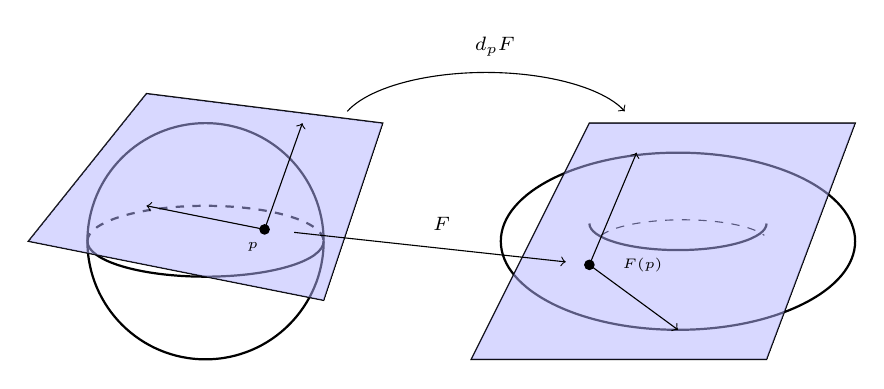
\begin{tikzpicture}[scale=1.5]
	% Esfera
	\draw [thick] (-1,0) arc (0:180:1 and -0.3);
	\draw [thick, dashed] (-3,0) arc (180:0:1 and 0.3);
	\draw [thick] (-2,0) circle (1);

	% Espacio Tangente a Esfera
	\draw [line width=0.5] (-3.5,0) -- (-2.5,1.25) -- (-0.5,1) -- (-1,-0.5) -- cycle;
	\draw [fill=blue!30!white,opacity=0.5, line width=0] (-3.5,0) -- (-2.5,1.25) -- (-0.5,1) -- (-1,-0.5) -- cycle;

	% Punto $a$
	\filldraw (-1.5,0.1) circle (0.04);
	\node at (-1.60,-0.05) {\tiny $p$};

	% Vector en $a$
	\draw [->] (-1.5,0.1) -- (-1.18,1);
	\draw [->] (-1.5,0.1) -- (-2.5,0.3);

	% Toro
	\draw [thick] (2,0) ellipse  (1.5 and 0.75);
	\draw [thick] (1.25,0.15) arc (0:-180:-0.75 and 0.225);
	\draw [dashed] (1.35,0.05) arc (20:160:-0.735 and 0.2);

	% Espacio tangente a Toro
	\draw [line width=0.5] (1.25,1) -- (3.5,1) -- (2.75,-1) -- (0.25,-1) -- cycle;
	\draw [fill=blue!30!white,opacity=0.5, line width=0] (1.25,1) -- (3.5,1) -- (2.75,-1) -- (0.25,-1) -- cycle;

	% Punto $F(a)$
	\filldraw (1.25,-0.2) circle (0.04);
	\node at (1.7,-0.2) {\tiny $F(p)$};

	% Vector en $F(a)$
	\draw[->] (1.25,-0.2) -- (1.65,0.75);
	\draw[->] (1.25,-0.2) -- (2,-0.75);

	% Lineas
	\draw[->] (-1.25,0.075) -- (1.05,-0.175);
	\node at (0,0.15) {\scriptsize $F$};


	\draw[->] (-0.8,1.1) arc (160:20:1.25 and 0.5);
	\node at (0.45,1.65) {\scriptsize $d_{p}F$};
\end{tikzpicture}

	\caption{Representación del diferencial de un mapa suave en un punto.}
\end{figure}

El diferencial $d_pF$ está bien definido dado que $F: M \to N$ y $f: N \to \R$ son funciones suaves, esto implica que $f \circ F: M \to \R$ será una función suave, por lo que $\omega(f \circ F)$ tiene sentido, la linealidad se tiene como consecuencia de que $\omega$ sea lineal y, por último, $d_pF(\omega): C^{\infty}(N) \to \R$ es una derivación en $F(p)$ dado que si $f, g \in C^{\infty}(N)$ entonces:

\begin{align*}
	d_pF(\omega)(fg) & = \omega((fg) \circ F)                                               \\
	                 & = \omega((f \circ F)(g \circ F))                                     \\
	                 & = (f \circ F)(p)\omega(g \circ F) + (g \circ F)(p) \omega(f \circ F) \\
	                 & = (f \circ F)(p)d_pF(\omega)(g) + (g \circ F)(p)d_pF(\omega)(f).
\end{align*}

A continuación, mostraremos algunas propiedades de los diferenciales de mapas suaves entre variedades, propiedades que son extensiones naturales de las propiedades conocidas de las derivadas totales del cálculo ordinario, como la linealidad del diferencial o la regla de la cadena.

\begin{lemma}\label{Lemma: Diferencial del Mapa Identidad}
	El diferencial del mapa identidad en una variedad es la identidad del espacio tangente a la variedad.
\end{lemma}

\begin{proof}
	Si $M$ es una variedad suave, $\id_M$ el mapa identidad en $M$, $p \in M$ un punto arbitrario y $\omega \in T_p(M)$ un vector tangente de $M$ en $p$, para cada $f \in C^{\infty}(M)$ se tiene:
	\begin{align*}
		d\id_{M}(\omega)(f) & = \omega(f \circ \id_M) = \omega(f).
	\end{align*}
	Dado que esto se cumple para cualquier $\omega \in T_p(M)$ y $f \in C^{\infty}(M)$, el diferencial será el mapa identidad en el espacio tangente.
\end{proof}

\begin{lemma}
	Si $M$ y $N$ son variedades suaves, $F: M \to N$ un mapa suave y $p \in M$ un punto arbitrario. El diferencial $d_pF: T_p(M) \to T_{F(p)}(M)$ es un operador lineal.
\end{lemma}

\begin{proof}
	Si $f,g \in C^{\infty}(N)$, $a \in \R$ y $\omega \in T_{p}(M)$, tenemos que:
	\begin{align*}
		d_pF(\omega)(af + g) & = \omega((af + g) \circ F)               \\
		                     & = \omega (af \circ F + g \circ F)        \\
		                     & = a\omega(f \circ F) + \omega(g \circ F) \\
		                     & = a d_pF (\omega)(f) + d_pF(\omega)(g).
	\end{align*}
	Por lo tanto, el diferencial de un mapa es un operador lineal.
\end{proof}

\begin{lemma}\label{Lemma: Regla de la Cadena para Diferenciales}
	Si $M$, $N$ y $P$ son variedades suaves, $F: M \to N$ y $G: N \to P$ mapas suaves y $p \in M$ un punto cualquiera, entonces el diferencial del mapa composición $G \circ F$ cumple la regla de la cadena, esto es,
	\[
		d_p(G \circ F) = d_{F(p)}G \circ d_pF
	\]
\end{lemma}

\begin{proof}
	Sea $\omega \in T_p(M)$ y $f \in C^{\infty}(P)$, tenemos que:
	\begin{align*}
		d_p(G \circ F) (\omega)(f) & = \omega(f \circ (G \circ F))       \\
		                           & = \omega ((f \circ G) \circ F)      \\
		                           & = d_pF(\omega)(f \circ G)           \\
		                           & = (d_{F(p)}G \circ d_pF)(\omega)(f)
	\end{align*}

	Por lo tanto, el diferencial de la composición cumple la regla de la cadena, más aún, es un mapa que lleva va del espacio tangente de $M$
	en $p$, $T_p(M)$, al espacio tangente de $P$ en $(G \circ F)(p)$, $T_{(G \circ F)(p)}(P)$.
\end{proof}

\begin{lemma}\label{Lemma: Diferencial de un Difeomorfismo}
	Si $M$ y $N$ son variedades suaves, $F: M \to N$ es un difeomorfismo y $p \in M$, entonces el diferencial $d_pF: T_p(M) \to T_{F(p)}(N)$ es un isomorfismo de espacios vectoriales y $(d_pF)^{-1} = d_{F(p)}(F^{-1})$.
\end{lemma}

\begin{proof}
	Dado que $F$ es un difeomorfismo, por definición $F$ es invertible por lo que existe una función $F^{-1}: N \to M$ tal que $F^{-1} \circ F = \id_M$ y $F \circ F^{-1} = \id_N$. Por los lemas probados anteriormente se tiene:
	\begin{align*}
		d_p(F^{-1} \circ F)      & = d_{F(p)}F^{-1} \circ d_pF = \id_{T_p(M)}       \\
		d_{F(p)}(F \circ F^{-1}) & = d_pF \circ d_{F(p)}F^{-1} = \id_{T_{F(p)}(N)}. \\
	\end{align*}
	Esto demuestra que tanto $d_pF$ como $d_{F(p)}F^{-1}$ son isomorfismos de espacios vectoriales dado que ambos son operadores lineales e invertibles, y además se comprueba que $(d_pF)^{-1} = d_{F(p)}F^{-1}$.
\end{proof}

De modo similar a la derivada total, el diferencial nos permitirá realizar cálculos en coordenadas locales, sin embargo, por cómo hemos definido al diferencial, estos operan sobre funciones definidas de manera global sobre la variedad. Al ser una generalización de la derivada total es de esperarse que puedan operar sin ambigüedad sobre subconjuntos abiertos, veremos esto a continuación.

\begin{lemma}
	Sea $M$ una variedad suave, $p \in M$ un punto arbitrario y $\omega \in T_{p}(M)$. Si $f,g \in C^{\infty}(M)$ coinciden en una vecindad de $p$, entonces $\omega(f) = \omega(g)$
\end{lemma}

\begin{proof}
	Definamos la función $h = f - g$, $h$ es una función suave que sea anula en una vecindad de $p$. Sea $\psi \in C^{\infty}(M)$ una función indicadora suave tal que $\psi(p) \equiv 1$ si $p \in \sup h$ y tal que $\sup \psi \subseteq M - \{p\}$. Dado que $\psi \equiv 1$ donde $h$ es diferente de cero, el producto $\psi h$ es idénticamente $h$. Y, como $h(p) = \psi(p) = 0$, por el lema \ref{Lemma: Propiedades De Las Derivaciones En Variedades} se tendrá que $\omega (h) = \omega (\psi h) = 0$.

	Por la linealidad de $\omega$ se sigue que $\omega(h) = \omega (f - g) = \omega(f) - \omega(g) = 0$, por lo tanto, $\omega(f) = \omega(g)$.
\end{proof}

\begin{lemma}\label{Lemma: Espacio Tangente a Subvariedad}
	Sea $M$ una variedad suave, $U \subseteq M$ un subconjunto abierto, y sea $\iota: U \to M$ el mapa de inclusión. Para cada $p \in U$, el diferencial $d_p\iota: T_p M \to T_pM$ es un isomorfismo de espacios vectoriales.
\end{lemma}

\begin{proof}
	Por el ejemplo \ref{Ex: Variedad Suave - Subvariedades Suaves} sabemos que $U$ es en sí misma una variedad suave por lo que no hay ambigüedad al considerar el espacio tangente en algún punto. La linealidad de la diferencial se tiene por definición de derivación.

	Para mostrar que el diferencial es inyectivo mostraremos que el kernel es nulo. Supongamos que $\omega \in T_{p}(U)$ y $d_p\iota(\omega) = 0 \in T_{p}(M)$. Sea $V$ una vecindad de $p$ tal que $\overline{V} \subset U$. Si $f: U \to \R$ es una función suave, por el lema \ref{Lemma: Lema de Extensión para Funciones Suaves} podemos garantizar que existe una función $\hat{f}: M \to \R$ que coincide con $f$ en $\overline{V}$. Luego, por el lema anterior se tiene que, como $f$ y $\hat{f}\big|_{U}$ son funciones suaves que coinciden en una vecindad de $p$, entonces:
	\begin{align*}
		\omega(f) & = \omega \left(\hat{f} \big|_{U} \right)\\
		          & = \omega(\hat{f} \circ \iota)   \\
		          & = d_p\iota(\omega)(\hat{f}) = 0
	\end{align*}

	Esto se cumplirá para cada función suave $f \in C^{\infty}(U)$, por lo que $\omega \equiv 0$, lo cual implica que $d\iota_p$ es inyectiva.

	Para mostrar que el diferencial del mapa de inclusión es sobreyectivo supongamos que $\omega \in T_p(M)$ es algún vector tangente arbitrario en $M$. Definamos al operador $\upsilon: C^{\infty}(U) \to \R$ de tal modo que $\upsilon(f) = \omega (\hat{f})$, donde $\hat{f}$ es cualquier función suave en $M$ que coincida con $f$ en $\overline{V}$, por el lema anterior $\upsilon(f)$ no depende de la elección de la función $\hat{f}$, por lo que $\upsilon$ está bien definida y es una derivación. Para cada función $g \in C^{\infty}(M)$ se cumple:
	\begin{align*}
		d_p\iota(\upsilon)(g)
		 & = \upsilon(g \circ \iota)                                  \\
		 & = \omega \left( (g \circ \iota) \big|_{V} \right) \\
		 & = \omega(g).
	\end{align*}
	Por lo tanto, $d\iota_p$ es un sobreyectivo, y por lo tanto será un isomorfismo entre los espacios vectoriales $T_p(U)$ y $T_p(M)$.
\end{proof}

\begin{theorem}[Invariancia de la Dimensión]\label{Teorema: Invariancia de la Dimensión}
	Si $M$ es una variedad suave, $n-$dimensional. Para cada $p \in M$, el espacio tangente $T_p(M)$ es un espacio vectorial $n-$dimensional.
\end{theorem}

\begin{proof}
	Para cada $p \in M$ podemos elegir una carta suave $(U, \phi)$ que contenga a $p$. Por definición $\phi$ es un difeomorfismo de $U$ a $\R^n$. El lema \ref{Lemma: Diferencial de un Difeomorfismo} nos dice que $T_{p}(U)$ y $T_{\phi(p)}(\R^n)$ son isomorfos, y el lema anterior garantiza que $T_{p}(U)$ y $T_{p}(M)$ también son isomorfos, por lo tanto, $T_{p}(M) \simeq T_{\phi(p)}(\R^n)$. De aquí que $\dim T_p(M) = \dim T_{\phi(p)}(\R^n) = n$.
\end{proof}

Una consecuencia inmediata del teorema \ref{Teorema: Isomorfismo entre Espacio Tangente y Espacio de Derivaciones} y el teorema anterior, \ref{Teorema: Invariancia de la Dimensión} es el siguiente corolario que nos da una identificación canónica de los elementos de cualquier espacio vectorial finito dimensional con los elementos de su espacio tangente, y, a su vez, dar una identificación canónica entre cada espacio tangente a un punto de una variedad y un espacio vectorial.

\begin{corollary}
	Sea $V$ un espacio vectorial finito dimensional con su estructura de variedad suave estándar. Para cada punto $a \in V$, el mapa $D_v: C^{\infty}(V) \to \R$ definido por:
	\[D_vf = \left. \frac{d}{dt} \right|_{t=0} f(a+tv), \]
	es un isomorfismo de $V$a $T_a(V)$.
\end{corollary}

\subsection{Vectores Tangentes en Coordenadas}\label{Subsección: Espacios Tangentes en Coordenadas}
Las ideas presentadas anteriormente nos son de mucha utilidad, dado que como veremos en esta sección los espacios tangentes y los diferenciales nos permiten realizar cálculos concretos en las variedades suaves.

Sean $M$ una variedad suave $n-$dimensional, $p \in M$ algún punto y $(U,\phi)$ una carta suave que contiene a $p$. Definiremos los mapas $\phi_i: U \to \R$ como $\phi_{i} = x_i \circ \phi$, donde $x_i$ son los elementos de la base estándar de $\R^n$.

Si $f$ es un mapa suave definido en una vecindad de $p$, tomaremos:
\[
	\left.
	\frac{\partial}{\partial \phi_i}
	\right|_{p} f
	=
	\left.
	\frac{\partial}{\partial x_i}
	\right|_{\phi(p)}
	\left( f \circ \phi^{-1} \right).
\]
Evidentemente cada $\frac{\partial}{\partial \phi_i}$ es una derivación, por lo que serán vectores tangentes en $T_p(M)$, y por definición $\phi: U \to \R^n$ es un difeomorfismo. Sabiendo esto y por el lema \ref{Lemma: Diferencial de un Difeomorfismo} podemos garantizar que el diferencial $d_p\phi: T_p(M) \to T_{\phi(p)}(\R^n)$ es un isomorfismo de espacios vectoriales.

\begin{lemma}\label{Lemma: Definicion Vector Coordenado}
	Sean $M$ una variedad suave, $p \in M$ un punto arbitrario y $(U,\phi) = (U, \phi_1, \dots, \phi_n)$ una carta suave que contiene a $p$, entonces:
	\[
		d_p\phi \left( \left. \frac{\partial }{\partial \phi_i}\right|_{p}\right)
    = \left. \frac{\partial}{\partial x_i} \right|_{\phi(p)}.
	\]
\end{lemma}

\begin{proof}
	Sea $f: \R^n \to \R$ cualquier función suave definida en una vecindad de $\phi(p)$, se tendrá que:
	\begin{align*}
		d_p\phi \left( \left. \frac{\partial}{\partial \phi_i} \right|_{p} \right) f
		 & = \left. \frac{\partial}{\partial \phi_i} \right|_{p}
		f \circ \phi                                                  \\
		 & = \left. \frac{\partial}{\partial x_i} \right|_{\phi(p)}
		f \circ \phi \circ \phi^{-1}                                  \\
		 & = \left. \frac{\partial}{\partial x_i}\right|_{\phi(p)} f.
	\end{align*}
\end{proof}

\begin{theorem}\label{Teorema: Base para el espacio tangente}
	Sean $M$ una variedad suave, $p \in M$ y $(U,\phi) = (U, \phi_1, \dots, \phi_n)$ una carta suave que contiene a $p$. El espacio tangente $T_p(M)$ tiene como base a la colección:
	\[
		\left. \frac{\partial}{\partial \phi_1} \right|_p, \hdots, \left. \frac{\partial}{\partial \phi_n} \right|_p .
	\]
\end{theorem}

\begin{proof}
	El corolario \ref{Corolario: Base de TpRn} nos dice que las derivadas parciales forman una base para $T_p(\R^n)$, además el lema anterior nos dice que el mapa:
	\begin{align*}
		d_p\phi: T_p(M)                                     & \to \T_{\phi(p)} (\R^n) \\
		\left. \frac{\partial}{\partial \phi_i} \right|_{p} & \mapsto
		\left. \frac{\partial}{\partial x_i} \right|_{\phi(p)},
	\end{align*}

	es un isomorfismo, y como los isomorfismos llevan bases de un espacio vectorial a bases de otros espacios vectoriales tendremos que el conjunto $\left\{ \frac{\partial}{\partial \phi_{i}}|_{p} \right\}_{i=1}^{n}$ es una base para $T_{p}(M)$.
\end{proof}

Como hemos mencionado, el diferencial de un mapa suave entre variedades ha sido de tal modo que este sea una generalización de la derivada total conocida del cálculo en $\R^n$, la cual puede ser representada por la matriz Jacobiana, sin embargo, una ventaja que tenemos con el diferencial es que es independiente de las coordenadas que se elijan, esto es, no depende de las bases que se pudiesen elegir para los espacios tangentes a las variedades. Aun así, es posible dar una representación matricial para el diferencial, evidentemente esta representación sí dependerá de las coordenadas elegidas.

Comenzaremos viendo que, en efecto, la representación matricial coincidirá con lo que se podría esperar en espacios euclidianos, esto es, que la matriz sea la matriz Jacobiana.

Consideremos dos espacios euclidianos $\R^n$ y $\R^m$, donde $\{x_1, \dots, x_n\}$ y $\{y_1, \dots, y_m\}$ son las bases estándar respectivas de cada espacio. Sean $U \subseteq \R^n$ y $V \subseteq \R^m$ subconjuntos abiertos, $p \in U$ un punto arbitrario y $F: U \to V$ una función suave. Utilizando la regla de la cadena para calcular el diferencial de $F$ en $p$ tenemos:
\begin{align*}
	d_{p}F
	\left(
	\left. \frac{\partial}{\partial x_i} \right|_{p}
	\right)
	 & =
	\left. \frac{\partial}{\partial x_i} \right|_{p} (f \circ F) \\
	 & =
	\sum_{j=1}^{n} \frac{\partial f}{\partial y_j} F(p)
	\frac{\partial F_j}{\partial x_i} (p)                        \\
	 & =
	\sum_{j=1}^{n}
	\left(
	\frac{\partial F_j}{\partial x_i} (p)
	\left.
	\frac{\partial}{\partial y_j}
	\right|_{F(p)}
	\right) f.                                                   \\
	\implies d_p F
	\left(
	\left. \frac{\partial}{\partial x_i} \right|_p
	\right)
	 & =
	\sum_{j=1}^{n}
	\frac{\partial F_j}{\partial x_i} (p)
	\left.
	\frac{\partial}{\partial y_j}
	\right|_{F(p)}.
\end{align*}
Por lo tanto, la representación matricial de $d_{p}F$ en términos de las bases elegidas para $\R^n$ y $\R^m$ es:

\[
	\begin{bmatrix}
		\frac{\partial F_1}{\partial x_1}(p) & \hdots & \frac{\partial F_1}{\partial x_n}(p) \\[24pt]
		\vdots                               & \ddots & \vdots                               \\[24pt]
		\frac{\partial F_m}{\partial x_1}(p) & \hdots & \frac{\partial F_m}{\partial x_n}(p)
	\end{bmatrix}.
\]

Esto es precisamente lo que cabría esperarse, que la representación en coordenadas del diferencial de una función suave sea precisamente la matriz Jacobiana, por lo que coincide con la derivada total.

Para ver qué sucede con el caso general consideremos dos variedades suaves $M$ y $N$, un punto $p \in M$ y un mapa suave $F: M \to N$. Tomemos dos cartas $(U,\phi)$ y $(V,\psi)$ que contengan a $p$ y $F(p)$ respectivamente.
\begin{figure}[h]
  \center
	\tikzexternaldisable % Desactiva el precompilado de figuras, ¡No quitar!
\begin{tikzcd}
	M \arrow[d, "\varphi"'] \arrow[r, "F"] & N \arrow[d, "\psi"] \\
	\mathbb{R}^m \arrow[r, "\hat{F}"']     & \mathbb{R}^n
\end{tikzcd}
\tikzexternalenable % Restaura la el precompilado de figuras.

	\caption*{Diagrama de la representación coordenada de un mapa.}
\end{figure}
Como se vio en la sección \ref{Sección: Mapas Suaves} el mapa $F$ tiene una representación en coordenadas dada por $\hat{F} = \psi \circ F \circ \phi^{-1}: \phi(U \cap F^{-1}(V)) \to \psi(V)$. Por los cálculos anterior podemos representar el diferencial de $\hat{F}$ en $\phi(p)$ con respecto a la base estándar por la matriz Jacobiana de $\hat{F}$ en $\phi(p)$. Utilizando el hecho de que $F \circ \phi^{-1} = \psi^{-1} \circ \hat{F}$, calculando obtenemos:
\begin{align*}
	d_{p}F \left( \left. \frac{\partial}{\partial \phi_i} \right|_{p}\right) & =
	d_p(\psi^{-1}\circ\hat{F}\circ \phi)\left(\left.\frac{\partial}{\partial \phi_i}\right |_p\right) \\
	                                                                         & =
	\left. d_p \psi^{-1} \right|_{\hat{F}(\phi(p))}
	\Biggl(
	d_{\phi(p)} \hat{F}
	\Biggl(
	\underbrace{d_p \phi
		\left(
		\left. \frac{\partial}{\partial \phi_i} \right|_{p}
		\right)}_{\left. \frac{\partial}{\partial x_i} \right|_{\phi (p)}}
	\Biggr)	\Biggr)                                                                                   \\
	                                                                         & =
	\left. d_p \psi^{-1} \right|_{\hat{F}(\phi(p))}
	\left(
	\sum_{j=1}^{n} \frac{\partial \hat{F_j}}{\partial x_i} \left( \phi(p) \right)
	\left. \frac{\partial}{\partial y_j} \right|_{F(\phi(p))}
	\right)                                                                                           \\
	                                                                         & =
	\sum_{j=1}^{n} \frac{\partial \hat{F}_j}{\partial x_i} (\phi(p))
	\left. d_p \psi^{-1} \right|_{\hat{F}(\phi(p))}
	\left(
	\left. \frac{\partial}{\partial y_j}\right|_{F(\phi(p))}
	\right)                                                                                           \\
	                                                                         & =
	\sum_{j=1}^{n} \frac{\partial \hat{F}_j}{\partial x_i} (\phi(p))
	\left.
	\frac{\partial}{\partial \psi_{j}}
	\right|_{\hat{F}(\phi(p))}.
\end{align*}

Por lo tanto, podemos representar el diferencial $dF_p$ con la matriz Jacobiana de la representación coordenada del mapa $F$.

Como estas representaciones dependen de la base elegida será necesario tener una manera en la que podamos transformar de unas coordenadas a otras. Consideremos una variedad suave $M$, dos cartas suaves $(U,\phi)=(U,\phi_1,\dots,\phi_n)$ y $(V,\psi)=(V,\psi_1,\dots,\psi_n)$, y un punto $p \in M$ que también pertenezca a la intersección $p \in U \cap V$. Los vectores tangentes en $p$ pueden ser representados respecto a las bases $\left\{\left. \frac{\partial}{\partial \phi_i} \right|_{p}\right\}_{i=1}^{n}$ y $\left\{\left. \frac{\partial}{\partial \psi_i} \right|_{p}\right\}_{i=1}^{n}$.

Naturalmente la representación de cualquier vector tangente está relacionada con cualquier otra representación, a continuación, veremos cómo es que las representaciones están relacionadas. Tomemos el diferencial del mapa de transición $\psi \circ \phi^{-1}: \phi(U \cap V) \to \R^n$.

\[
	d_{\phi(p)}(\psi \circ \phi^{-1}) \left( \left. \frac{\partial}{\partial \phi_{i}} \right|_{\phi(p)} \right) = \sum_{j=1}^{n}\frac{\partial \psi_j}{\partial \phi_i} (\phi(p)) \left. \frac{\partial}{\partial \psi_{j}} \right|_{\psi(p)}.
\]

Una consecuencia inmediata del lema \ref{Lemma: Definicion Vector Coordenado} es la siguiente representación de los vectores tangentes, de la cual, junto con la identidad anterior se seguirá la cadena de igualdades:

\begin{align*}
	\left. \frac{\partial}{\partial \phi_i}\right|_{p}
	 & =
	d_{\phi(p)} \left(\phi^{-1}\right)
	\left(\left.
	\frac{\partial}{\partial \phi_i}
	\right|_{\phi(p)}\right)                                            \\
	 & =
	d_{\psi(p)}(\psi^{-1}) \circ d_{\phi(p)}\left(\psi \circ \phi^{-1}\right)
	\left( \left.
	\frac{\partial}{\partial \phi_i}
	\right|_{\phi(p)}\right)                                            \\
	 & =
	d_{\psi(p)}(\psi^{-1}) \left(
	\sum_{j=1}^{n}\frac{\partial \psi_j}{\partial \phi_i}(\phi(p))
	\left.
	\frac{\partial}{\partial \psi_j}
	\right|_{\psi(p)} \right)                                           \\
	 & = \sum_{j=1}^{n}\frac{\partial \psi_j}{\partial \phi_i}(\phi(p))
	\left.
	\frac{\partial}{\partial \psi_j}
	\right|_{p}.
\end{align*}

Por lo tanto, si tenemos un vector tangente $\omega \in T_p(M)$ con dos representaciones diferentes, digamos:
\[
	\omega = \sum_{i=1}^{n} v_i \frac{\partial}{\partial \phi_i}
	\quad \text{y} \quad
	\omega = \sum_{j=1}^{n} w_j \frac{\partial}{\partial \psi_j}.
\]
Donde $v_i$ y $w_i$ son constantes que dependen de $\omega$, y podemos transformar las constantes del siguiente modo:
\[
	w_j = \sum_{i=1}^{n} \frac{\partial \psi_j}{\partial \phi_i} (\phi(p)) v_i.
\]

\begin{example}
	Consideremos el mapa de transición entre las coordenadas esféricas y las coordenadas estándar en subconjuntos abiertos adecuados de $\R^{3}$, el cual está por la igualdad $(x,y,z) = (r \cos \phi \sin \theta, r \sin \phi \sin \theta, r\cos \theta)$. Tomemos el punto $p \in \R^{3}$ con representación en coordenadas esféricas $p = (r,\theta,\phi) = (2,\frac{\pi}{4},\frac{\pi}{4})$ y tomemos un vector tangente $\omega \in T_p(\R^3)$ cuya representación en coordenadas polares esté dada por:
	\[
		\omega = \left. \frac{\partial}{\partial r} \right|_p -
		\left. 2\frac{\partial}{\partial \theta} \right|_p +
		\left. 3\frac{\partial}{\partial \phi} \right|_p.
	\]
	Si queremos transformar este vector tangente a coordenadas estándar necesitaremos utilizar la fórmula que acabamos de deducir de cambio de coordenadas. Calculando las constantes $v_i$:
	\begin{align*}
		v_1 & =
		\left. \frac{\partial}{\partial r} r\cos(\phi)\sin(\theta) \right|_p
		\frac{\partial}{\partial x} +
		\left. \frac{\partial}{\partial r} r\sin(\phi)\sin(\theta)\right|_p
		\frac{\partial}{\partial y} +
		\left. \frac{\partial}{\partial r}r\cos(\theta)\right|_{p}
		\frac{\partial}{\partial z}                                          \\
		    & = \cos(\phi)\sin(\theta)|_p \frac{\partial}{\partial x}
		+ \sin(\phi)\sin(\theta)|_p  \frac{\partial}{\partial y}
		+ \cos(\theta)|_p \frac{\partial}{\partial z}                        \\
		    & = \frac{1}{2} \frac{\partial}{\partial x}
		+ \frac{1}{2} \frac{\partial}{\partial y}
		+ \frac{\sqrt{2}}{2} \frac{\partial}{\partial z}.                    \\
		v_2 & =
		\left. \frac{\partial}{\partial \theta} r\cos(\phi)\sin(\theta) \right|_p
		\frac{\partial}{\partial x} +
		\left. \frac{\partial}{\partial \theta} r\sin(\phi)\sin(\theta)\right|_p
		\frac{\partial}{\partial y} +
		\left. \frac{\partial}{\partial \theta}r\cos(\theta)\right|_{p}
		\frac{\partial}{\partial z}                                          \\
		    & = r\cos(\phi)\cos(\theta)|_p \frac{\partial}{\partial x}
		+ r\sin(\phi)\cos(\theta)|_p  \frac{\partial}{\partial y}
		- r\sin(\theta)|_p \frac{\partial}{\partial z}                       \\
		    & = \frac{\partial}{\partial x} + \frac{\partial }{\partial y}
		- \frac{\partial}{\partial z}.                                       \\
		v_3 & =
		\left. \frac{\partial}{\partial \phi} r\cos(\phi)\sin(\theta) \right|_p
		\frac{\partial}{\partial x} +
		\left. \frac{\partial}{\partial \phi} r\sin(\phi)\sin(\theta)\right|_p
		\frac{\partial}{\partial y} +
		\left. \frac{\partial}{\partial \phi} r\cos(\theta)\right|_{p}
		\frac{\partial}{\partial z}                                          \\
		    & = -r\sin(\phi)\sin(\theta)|_p \frac{\partial}{\partial x}
		+ r\cos(\phi)\sin(\theta)|_p  \frac{\partial}{\partial y}            \\
		    & = - \frac{\partial}{\partial x} + \frac{\partial}{\partial y}.
	\end{align*}
	Por lo tanto, podemos sustituir en la ecuación que nos da el vector tangente para obtener su representación en coordenadas estándar, obteniendo:
	\[ \omega =
		\left. -\frac{9}{2} \frac{\partial}{\partial x} \right|_p +
		\left. \frac{3}{2}\frac{\partial}{\partial y} \right|_p +
		\left. \frac{\sqrt{2} - 4}{2} \frac{\partial}{\partial z} \right|_p .\]
\end{example}


\subsection{El Fibrado Tangente}\label{Subsección: Fibrado Tangente}
Por la definición que hemos dado de espacio tangente, estos están definidos en cada punto de una variedad suave, sin embargo, para algunos fines es más conveniente considerar todos los espacios tangentes a una variedad de forma simultánea. Es con este propósito que definiremos al Fibrado Tangente de una variedad suave, este objeto nos dará una manera de organizar los espacios tangentes de una variedad suave de tal modo que el objeto resultante sea en sí mismo una variedad suave.

\begin{center}
	\begin{figure}[h!]
		\centering
		\begin{subfigure}{0.35\textwidth}
			\centering
			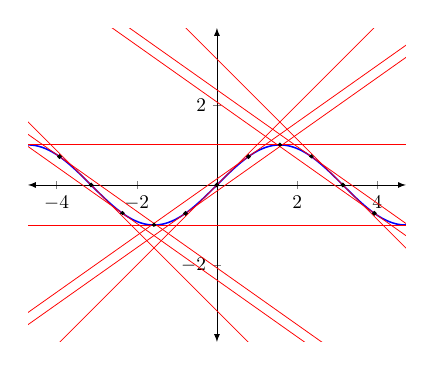
\begin{tikzpicture}[scale=0.70]
	\begin{axis}[
			% grid=both,
			xmin=-3*pi/2,
			xmax=3*pi/2,
			ymin=-1.6,
			ymax=1.6,
			axis lines=middle,
			axis line style={latex-latex},
			axis equal,
		]

		\addplot[
			samples=200,
			domain=-4*pi:4*pi,
			color=blue,
			thick,
			smooth,
		]
		{sin(deg(x))};
\addplot[domain=-5:5,color=red,thin]{-0.707107 * (x + 3.926991) + 0.707107};
\addplot+[mark=*, mark options={black},mark size=1pt] coordinates {( -3.926991 , 0.707107 )};
\addplot[domain=-5:5,color=red,thin]{-1.000000 * (x + 3.141593) + -0.000000};
\addplot+[mark=*, mark options={black},mark size=1pt] coordinates {( -3.141593 , -0.000000 )};
\addplot[domain=-5:5,color=red,thin]{-0.707107 * (x + 2.356194) + -0.707107};
\addplot+[mark=*, mark options={black},mark size=1pt] coordinates {( -2.356194 , -0.707107 )};
\addplot[domain=-5:5,color=red,thin]{0.000000 * (x + 1.570796) + -1.000000};
\addplot+[mark=*, mark options={black},mark size=1pt] coordinates {( -1.570796 , -1.000000 )};
\addplot[domain=-5:5,color=red,thin]{0.707107 * (x + 0.785398) + -0.707107};
\addplot+[mark=*, mark options={black},mark size=1pt] coordinates {( -0.785398 , -0.707107 )};
\addplot[domain=-5:5,color=red,thin]{1.000000 * (x - 0.000000) - -0.000000};
\addplot+[mark=*, mark options={black},mark size=1pt] coordinates {( 0.000000 , 0.000000 )};
\addplot[domain=-5:5,color=red,thin]{0.707107 * (x - 0.785398) - -0.707107};
\addplot+[mark=*, mark options={black},mark size=1pt] coordinates {( 0.785398 , 0.707107 )};
\addplot[domain=-5:5,color=red,thin]{-0.000000 * (x - 1.570796) - -1.000000};
\addplot+[mark=*, mark options={black},mark size=1pt] coordinates {( 1.570796 , 1.000000 )};
\addplot[domain=-5:5,color=red,thin]{-0.707107 * (x - 2.356195) - -0.707107};
\addplot+[mark=*, mark options={black},mark size=1pt] coordinates {( 2.356195 , 0.707107 )};
\addplot[domain=-5:5,color=red,thin]{-1.000000 * (x - 3.141593) - 0.000000};
\addplot+[mark=*, mark options={black},mark size=1pt] coordinates {( 3.141593 , -0.000000 )};
\addplot[domain=-5:5,color=red,thin]{-0.707107 * (x - 3.926991) - 0.707107};
\addplot+[mark=*, mark options={black},mark size=1pt] coordinates {( 3.926991 , -0.707107 )};	\end{axis}
\end{tikzpicture}

		\end{subfigure}
		\hspace{40pt}
		\begin{subfigure}{0.35\textwidth}
			\centering
			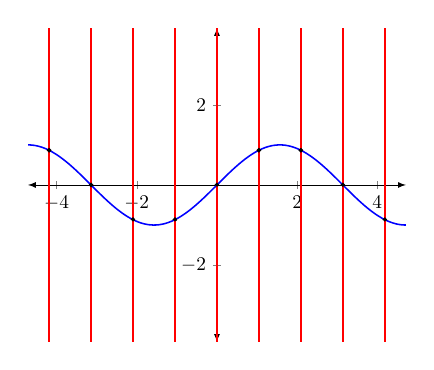
\begin{tikzpicture}[scale=0.70]
	\begin{axis}[
			% grid=both,
			xmin=-3*pi/2,
			xmax=3*pi/2,
			ymin=-1.6,
			ymax=1.6,
			axis lines=middle,
			axis line style={latex-latex},
			axis equal,
		]

		\addplot[
			samples=200,
			domain=-4*pi:4*pi,
			color=blue,
			thick,
			smooth,
		]
		{sin(deg(x))};

\addplot+[mark=*, mark options={black},mark size=1pt] coordinates {( -4.188790 , 0.866025 )};
\addplot[thick, smooth,domain=-pi:pi,red] coordinates {(-4.188790,-5)(-4.188790,5)};
\addplot+[mark=*, mark options={black},mark size=1pt] coordinates {( -3.141593 , -0.000000 )};
\addplot[thick, smooth,domain=-pi:pi,red] coordinates {(-3.141593,-5)(-3.141593,5)};
\addplot+[mark=*, mark options={black},mark size=1pt] coordinates {( -2.094395 , -0.866025 )};
\addplot[thick, smooth,domain=-pi:pi,red] coordinates {(-2.094395,-5)(-2.094395,5)};
\addplot+[mark=*, mark options={black},mark size=1pt] coordinates {( -1.047197 , -0.866025 )};
\addplot[thick, smooth,domain=-pi:pi,red] coordinates {(-1.047197,-5)(-1.047197,5)};
\addplot+[mark=*, mark options={black},mark size=1pt] coordinates {( 0.000000 , 0.000000 )};
\addplot[thick, smooth,domain=-pi:pi,red] coordinates {(0.000000,-5)(0.000000,5)};
\addplot+[mark=*, mark options={black},mark size=1pt] coordinates {( 1.047198 , 0.866025 )};
\addplot[thick, smooth,domain=-pi:pi,red] coordinates {(1.047198,-5)(1.047198,5)};
\addplot+[mark=*, mark options={black},mark size=1pt] coordinates {( 2.094395 , 0.866025 )};
\addplot[thick, smooth,domain=-pi:pi,red] coordinates {(2.094395,-5)(2.094395,5)};
\addplot+[mark=*, mark options={black},mark size=1pt] coordinates {( 3.141593 , -0.000000 )};
\addplot[thick, smooth,domain=-pi:pi,red] coordinates {(3.141593,-5)(3.141593,5)};
\addplot+[mark=*, mark options={black},mark size=1pt] coordinates {( 4.188790 , -0.866026 )};
\addplot[thick, smooth,domain=-pi:pi,red] coordinates {(4.188790,-5)(4.188790,5)};	

\end{axis}
\end{tikzpicture}

		\end{subfigure}
		\\[20pt]
		\begin{subfigure}{0.35\textwidth}
			\centering
			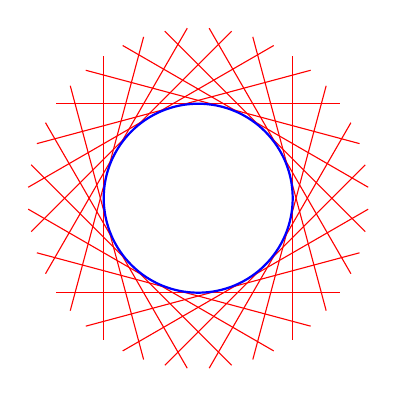
\begin{tikzpicture}[scale=1.20]
  % Lineas iniciales
  \draw[red] (-1,-1.5) -- (-1,1.5);
  \draw[red] (1,-1.5)  -- (1,1.5);
  \draw[red] (-1.5,1)  -- (1.5,1);
	\draw[red] (-1.5,-1) -- (1.5,-1);

	\begin{scope}[rotate around={15:(0,0)}]
		\draw[red] (-1,-1.5) -- (-1,1.5);
		\draw[red] (1,-1.5)  -- (1,1.5);
		\draw[red] (-1.5,1)  -- (1.5,1);
		\draw[red] (-1.5,-1) -- (1.5,-1);
	\end{scope}
	\begin{scope}[rotate around={30:(0,0)}]
		\draw[red] (-1,-1.5) -- (-1,1.5);
		\draw[red] (1,-1.5)  -- (1,1.5);
		\draw[red] (-1.5,1)  -- (1.5,1);
		\draw[red] (-1.5,-1) -- (1.5,-1);
	\end{scope}
	\begin{scope}[rotate around={45:(0,0)}]
		\draw[red] (-1,-1.5) -- (-1,1.5);
		\draw[red] (1,-1.5)  -- (1,1.5);
		\draw[red] (-1.5,1)  -- (1.5,1);
		\draw[red] (-1.5,-1) -- (1.5,-1);
	\end{scope}
	\begin{scope}[rotate around={60:(0,0)}]
		\draw[red] (-1,-1.5) -- (-1,1.5);
		\draw[red] (1,-1.5)  -- (1,1.5);
		\draw[red] (-1.5,1)  -- (1.5,1);
		\draw[red] (-1.5,-1) -- (1.5,-1);
	\end{scope}
	\begin{scope}[rotate around={75:(0,0)}]
		\draw[red] (-1,-1.5) -- (-1,1.5);
		\draw[red] (1,-1.5)  -- (1,1.5);
		\draw[red] (-1.5,1)  -- (1.5,1);
		\draw[red] (-1.5,-1) -- (1.5,-1);
	\end{scope}

	\draw[blue,thick] (0,0) circle (1);
\end{tikzpicture}

		\end{subfigure}
		\hspace{30pt}
		\begin{subfigure}{0.35\textwidth}
			\centering
			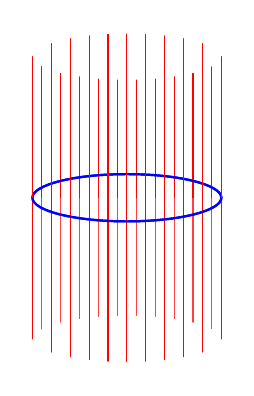
\begin{tikzpicture}[scale=1.20]
  \path[use as bounding box] (-1.05,-1.8) rectangle (1.05,1.8);

	% Lineas Traseras
	\draw[color=red,opacity=0.75] (0.1,-2.0) -- (0.1,0.0);
	\draw[color=red,opacity=0.75] (0.3,-2.0) -- (0.3,0.0);
	\draw[color=red,opacity=0.75] (0.5,-2.0) -- (0.5,0.0);
	\draw[color=red,opacity=0.75] (0.7,-2.0) -- (0.7,0.0);
	\draw[color=red,opacity=0.75] (0.9,-2.0) -- (0.9,0.0);
	\draw[color=red,opacity=0.75] (-0.1,-2.0) -- (-0.1,0.0);
	\draw[color=red,opacity=0.75] (-0.3,-2.0) -- (-0.3,0.0);
	\draw[color=red,opacity=0.75] (-0.5,-2.0) -- (-0.5,0.0);
	\draw[color=red,opacity=0.75] (-0.7,-2.0) -- (-0.7,0.0);
	\draw[color=red,opacity=0.75] (-0.9,-2.0) -- (-0.9,0.0);
	\fill[white] (-1,-1.5) arc (0:180:-1 and 0.25) -- (1,-2) -- (-1,-2)--(-1,-1.5);

	% Elipse
	\draw[blue,thick] (0,0) ellipse (1 and 0.25);

	% Lineas Frontales
	\draw[red] (0.0,-2.0) -- (0.0,0.0);
	\draw[red] (0.2,-2.0) -- (0.2,0.0);
	\draw[red] (0.4,-2.0) -- (0.4,0.0);
	\draw[red] (0.6,-2.0) -- (0.6,0.0);
	\draw[red] (0.8,-2.0) -- (0.8,0.0);
	\draw[red] (1.0,-2.0) -- (1.0,0.0);
	\draw[red] (-0.2,-2.0) -- (-0.2,0.0);
	\draw[red] (-0.4,-2.0) -- (-0.4,0.0);
	\draw[red] (-0.6,-2.0) -- (-0.6,0.0);
	\draw[red] (-0.8,-2.0) -- (-0.8,0.0);
	\draw[red] (-1.0,-2.0) -- (-1.0,0.0);

  \draw[thick,white,fill=white] (-1,-1.50) arc (0:180:-1 and -0.25) -- (1,-2) -- (-1,-2) -- cycle;

	\begin{scope}[rotate around={180:(0,0)}]
	\draw[red] (0.1,-2.0) -- (0.1,0.0);
	\draw[red] (0.3,-2.0) -- (0.3,0.0);
	\draw[red] (0.5,-2.0) -- (0.5,0.0);
	\draw[red] (0.7,-2.0) -- (0.7,0.0);
	\draw[red] (0.9,-2.0) -- (0.9,0.0);
	\draw[red] (-0.1,-2.0) -- (-0.1,0.0);
	\draw[red] (-0.3,-2.0) -- (-0.3,0.0);
	\draw[red] (-0.5,-2.0) -- (-0.5,0.0);
	\draw[red] (-0.7,-2.0) -- (-0.7,0.0);
	\draw[red] (-0.9,-2.0) -- (-0.9,0.0);
	\fill[white] (-1,-1.5) arc (0:180:-1 and 0.25) -- (1,-2) -- (-1,-2)--(-1,-1.5);

	% Elipse
	\draw[blue,thick] (0,0) ellipse (1 and 0.25);

	% Lineas Frontales
	\draw[red] (0.0,-2.0) -- (0.0,0.0);
	\draw[red] (0.2,-2.0) -- (0.2,0.0);
	\draw[red] (0.4,-2.0) -- (0.4,0.0);
	\draw[red] (0.6,-2.0) -- (0.6,0.0);
	\draw[red] (0.8,-2.0) -- (0.8,0.0);
	\draw[red] (1.0,-2.0) -- (1.0,0.0);
	\draw[red] (-0.2,-2.0) -- (-0.2,0.0);
	\draw[red] (-0.4,-2.0) -- (-0.4,0.0);
	\draw[red] (-0.6,-2.0) -- (-0.6,0.0);
	\draw[red] (-0.8,-2.0) -- (-0.8,0.0);
	\draw[red] (-1.0,-2.0) -- (-1.0,0.0);

	\draw[thick,white,fill=white] (-1,-1.5) arc (0:180:-1 and -0.25) -- (1,-2) -- (-1,-2) -- cycle;
	\end{scope}
\end{tikzpicture}

		\end{subfigure}
    \caption{Representación del fibrado tangente de dos variedades, $\sin(x)$ y $\S^{1}$.}
  \end{figure}
\end{center}

\begin{definition}[Fibrado Tangente]
	Dada una variedad suave $M$, definimos el \it{fibrado tangente de $M$} o \it{haz tangente de $M$}, el cual denotaremos por $TM$, como la unión disjunta de todos los espacios tangentes a $M$:
	\[ TM = \bigsqcup_{p \in M} T_p(M) = \bigcup_{p \in M} \{p\} \times T_p(M). \]
\end{definition}

Denotaremos a los elementos del conjunto como un par ordenado $(p, \omega)$, donde $p \in M$ y $\omega \in T_p(M)$. El fibrado tangente $TM$ tiene un mapa proyección natural sobre la variedad $M$, $\pi: TM \to M$ dado por $\pi(p,\omega)=p$.

\begin{theorem}\label{Teorema: Estructura de Variedad del Fibrado Tangente}
	Sea $M^n$ una variedad suave, el fibrado tangente $TM$ tiene una topología natural y una estructura suave que vuelven a $TM$ una variedad suave $2n-$dimensional de tal modo que la proyección $\pi: TM \to M$ es suave con respecto a dicha estructura suave.
\end{theorem}

\begin{proof}
	Para realizar esta demostración haremos uso del lema \ref{Lemma: Lema de Cartas Suaves de una Variedad}, mostraremos que $TM$ cumple las cinco propiedades ahí mencionadas cuando se da una colección adecuada de subconjuntos.

	Consideremos una carta suave $(U,\phi)=(U,\phi_1,\dots,\phi_n)$ de $M$, $\pi^{-1}(U) \subseteq TM$ será la colección formada por todos los vectores tangentes a $M$ en cada punto de $U$. Dado que cada $T_p(M)$ es un espacio vectorial y que, como hemos visto, $\{\left. \frac{\partial}{\partial \phi_{i}} \right|_{p}\}_{i=1}^{n}$ nos da una base para $T_p(M)$, cada vector tangente $\omega_p \in T_p(M)$ podrá ser escrito de forma única como una combinación lineal:
	\[
		\omega_p = \sum_{i=1}^{n} v_i \left. \frac{\partial}{\partial \phi_{i}}\right|_{p},
	\]
	donde cada $v_i$ es una constante que dependerá del vector tangente, $v_i = v_i(\omega_p) \in \R$. Definamos el mapa $\hat{\phi}: TM \to \R^{2n}$ como:
	\[
		\hat{\phi} \left(\sum_{i=1}^{n} v_i
		\left. \frac{\partial}{\partial \phi_{i}}\right|_{p} \right)
		=
		\left(\phi_1(p), \dots, \phi_n(p), v_1, \dots, v_n \right).
	\]
a
	Por cómo estamos definiendo este mapa, la imagen de $\pi^{-1}(U)$ bajo $\hat{\phi}$, $\hat{\phi}(\pi^{-1})(U)$ será el conjunto $\phi(U) \times \R^n$, que es un subconjunto abierto de $\R^{2n}$, y trivialmente será una biyección dado que el mapa inverso existe, de hecho, este puede ser escrito explícitamente como:
	\[
		\hat{\phi}^{-1}(\phi_{1},\dots, \phi_{n}, v_1, \dots, v_n)
		=
		\sum_{i=1}^{n} v_i \left. \frac{\partial}{\partial \phi_i} \right|_{\phi^{-1}(p)}.
	\]
	Por lo tanto, la condición 1 del lema se cumple.

	Para mostrar la segunda propiedad tomemos dos cartas suaves en $M$, $(U,\phi)$ y $(V,\psi)$, existirán cartas $(\pi^{-1}(U),\hat{\phi})$ y $(\pi^{-1}(V),\hat{\psi})$ en $TM$ correspondientes a las respectivas cartas en $M$. Notemos que, sin importar si la intersección es vacía se tiene que $\phi(U \cap V)$ y $\psi(U \cap V)$ son subconjuntos abiertos de $\R^n$, por lo que:
	\begin{align*}
		\hat{\phi}(\pi^{-1}(U) \cap \pi^{-1}(V)) & =
		\phi(U \cap V) \times \R^n,                  \\
		\hat{\psi}(\pi^{-1}(U) \cap \pi^{-1}(V)) & =
		\psi(U \cap V) \times \R^n.                  \\
	\end{align*}
	Son subconjuntos abiertos de $\R^{2n}$, esto implica que la propiedad 2 se cumple para estas cartas en $TM$.

	El mapa de transición $\hat{\psi} \circ \hat{\phi}^{-1}: \phi(U \cap V) \times \R^n \to \psi(U \cap V) \times \R^n$ puede ser expresado de manera explícita utilizando la identidad para el cambio de coordenadas mostrada en la sección anterior.
	\begin{align*}
		\hat{\psi} \circ \hat{\phi}^{-1}
		(\phi_1, \dots, \phi_n, v_1, \dots, v_n)
		 & =
		\hat{\psi} \left( \left.
		\sum_{i=1}^{n} v_i \frac{\partial}{\partial \phi_i}
		\right|_{\phi^{-1}(p)}\right)                      \\
		 & =
		\hat{\psi}\left(
		\sum_{i=1}^{n}
		\left(
		\sum_{j=1}^{n}
		\frac{\partial \psi_i}{\partial \phi_j} (\phi(p)) w_j
		\right)
		\left.
		\frac{\partial}{\partial \phi_i}
		\right|_{\phi^{-1}(p)}
		\right)
		\\
		 & =
		\Biggl(
		\psi_1(\phi^{-1}(p)), \dots, \psi_n(\phi^{-1}(p)), \\
		 & \quad \hspace{24pt}
		\sum_{j=1}^{n} \frac{\partial \psi_1}{\partial \phi_j}(\phi(p))w_j,
		\dots,
		\sum_{j=1}^{n} \frac{\partial \psi_n}{\partial \phi_j}(\phi(p))w_j
		\Biggr).
	\end{align*}
	Por lo tanto, cada una de las componentes es la composición de mapas suaves o la suma de mapas suaves, por lo que el mapa $\hat{\psi} \circ \phi^{-1}$ es suave, cumpliendo así la propiedad 3.

	Por la segundo numerabilidad de $M$ podemos elegir una colección numerable $\mathcal{U} = \{U_\alpha\}$ de cartas coordenadas, de la cual obtendremos la colección numerable $\{\pi^{-1}(U_\alpha)\}$ de cartas coordenadas que cubren a $TM$ y que como hemos visto cumplen las propiedades 1, 2 y 3, y la existencia de tal colección nos da la cuarta propiedad.

	Para la quinta y última propiedad notemos que si se damos dos elementos $(p,\omega)$ y $(q, \nu)$ de $TM$ entonces hay dos posibilidades, $p = q$, en cuyo caso habrá una vecindad $\pi^{-1}(U)$ que contiene a ambos o $p \neq q$, en cuyo caso existan vecindades disjuntas $U,V$ en $M$ tales que $p \in U$ y $q \in V$, de modo que $\pi^{-1}(U)$ y $\pi^{-1}(V)$ serán vecindades disjuntas de $(p,\omega)$ y $(q,\nu)$.

	Por lo tanto, podemos concluir que $TM$ es una variedad suave con la estructura suave dada por los conjuntos de la forma $\pi^{-1}(U)$. La suavidad de la proyección se garantiza por el teorema \ref{Teorema: Mapa a Producto de Variedades Suaves}.
\end{proof}

A las componentes del mapa $\hat{\phi}: TM \to \R^{2n}$ que hemos definido le llamaremos las \it{coordenadas naturales en $TM$}, este mapa es un difeomorfismo y da lugar al siguiente corolario.

\begin{corollary}
	Si $M^n$ es una variedad suave y $M$ puede ser cubierto por una única carta suave, entonces existe un difeomorfismo entre $TM$ y $M \times \R^n$.
\end{corollary}

Es importante tener claro que, si bien para algunas variedades es posible visualizar su fibrado tangente como el producto cartesiano de la variedad con $\R^n$ y esto nos da una cierta intuición de su estructura suave, como es el caso del fibrado tangente de $\R^n$, el cual será difeomorfas a $\R^{2n}$ o el fibrado tangente de $\S^{1}$, el cual es posible visualizar como un cilindro, no siempre es posible visualizar a los fibrados tangentes como el producto de variedades ya que los difeomorfismo no siempre están definidos de manera global.

Ahora podemos considerar qué es lo que sucede cuando tomamos el diferencial en cada uno de los puntos de un mapa suave $F: M \to N$, donde $M$ y $N$, evidentemente este tendría que ser un mapa que vaya del fibrado tangente de $M$ al fibrado tangente de $N$, esto es, el diferencial de $F$ en cada punto de $M$, al cual llamaremos \it{diferencial global} es un mapa $dF: TM \to TN$, y como extensión que es del diferencial en un punto se tendría que al restringirnos a un espacio tangente particular $T_p(M)$, el diferencial global $dF$ coincidirá con el diferencial de $F$ en $p$, $d_{p}F$.

\begin{figure}[h]
	\adjustbox{scale=1.5,center}
	{
		\tikzexternaldisable % Desactiva el precompilado de figuras, ¡No quitar!
\begin{tikzcd}
  M \arrow[r, "F"]                       & N                      \\[12pt]
	TM \arrow[r, "dF"'] \arrow[u, "\pi_M"] & TN \arrow[u, "\pi_N"']
\end{tikzcd}
\tikzexternalenable % Restaura la el precompilado de figuras.

	}
	\caption*{Diagrama del diferencial global de un mapa entre dos variedades.}
\end{figure}

\begin{theorem}
	Si $M^{n}$ y $N^{k}$ son variedades suaves y $F: M \to N$ es un mapa suave, el diferencial global $dF: TM \to TN$ es un mapa suave.
\end{theorem}

\begin{proof}
	Como se vio hace unos párrafos, el diferencial de $F$ en un punto $p$, $dF_p$ tiene una representación coordenada como:
	\[
		d_{p}F \left( \left. \frac{\partial}{\partial x_i} \right|_{p}\right)
		=
		\sum_{i=1}^{n} \frac{\partial \hat{F}_j}{\partial x_i} (\phi(p)) \left. \frac{\partial}{\partial y_j} \right|_{F(p)}.
	\]

	Donde $\phi$ es un difeomorfismo entre una vecindad del punto $p \in M$ y $\R^n$, por tanto, utilizando las coordenadas naturales en $TM$ podemos representar al diferencial como:

	\[
		dF(x_1, \dots, x_n, \omega_1, \dots, \omega_n) =
		\left(
		F_1(p), \dots, F_k(p), \sum_{i=1}^{n} \frac{\partial F_1}{\partial x_i}(p) \frac{\partial}{\partial y_1}, \dots, \sum_{i=1}^{n} \frac{\partial F_k}{\partial x_i} (p)\frac{\partial}{\partial y_k}
		\right).
	\]

	Cada una de las componentes serán suaves dado que $F$ es suave por hipótesis, por lo tanto $dF$ es un mapa suave.
\end{proof}

Un sencillo corolario que extiende las propiedades ya vistas del diferencial en un punto al diferencial global y que es consecuencia de los lemas \ref{Lemma: Diferencial del Mapa Identidad}, \ref{Lemma: Regla de la Cadena para Diferenciales} y \ref{Lemma: Diferencial de un Difeomorfismo} es el siguiente.

\begin{corollary}\label{Corolario: Propiedades de los diferenciales}
	Sean $M$, $N$ y $P$ variedades suaves y sean $F: M \to N$ y $G: N \to P$ mapas suaves, entonces:
	\begin{itemize}
		\item $d(G \circ F) = dG \circ dF$.
		\item $d(\id_M) = \id_{TM}$.
		\item Si $F$ es un difeomorfismo, entonces $dF: TM \to TN$ es un difeomorfismo, y $(dF)^{-1} = d(F^{-1})$.
	\end{itemize}
\end{corollary}

\subsection{Curvas En Variedades}\label{Subsección: Curvas En Variedades}
Una de las ideas que podemos trasladar del cálculo ordinario al cálculo que estamos realizando en variedades suaves es la idea de curva definida en una superficie y la velocidad de la misma, nombre que viene inspirado de la utilidad en la física que estos conceptos tiene, ya que podemos pensar en la curva como una trayectoria y su derivada como su velocidad.
En nuestro caso al estar trabajando con variedades estas serán nuestras \enquote{superficies} y, si bien no podemos simplemente derivar, sí podemos asociar a cada punto de la curva un vector en el espacio tangente.

\begin{definition}[Curva en una Variedad]
  \label{Definición: Curva en Variedades}
	Sea $M$ una variedad y sea $\gamma: I \subset \R \to M$ un mapa continuo, donde $I$ es un intervalo abierto, diremos que $\gamma$ es una \it{curva sobre $M$}. Además, si el mapa $\gamma: I \subset \R \to M$ es suave diremos que $\gamma$ es una curva suave.
\end{definition}

Notemos que para la definición de curva solo estamos pidiendo continuidad, no suavidad. Una curva puede estar definida en una variedad topológica para la cual no es posible dar una estructura suave. Sin embargo, para poder definir la velocidad es necesario que el espacio tangente esté definido, por lo que pediremos que tanto las variedades como las curvas sean suaves.

\begin{definition}[Velocidad de una Curva]
	Sea $M$ una variedad suave, $\gamma: I \to M$ una curva suave y $t_0 \in I$. Definimos la \it{velocidad de $\gamma$ en $t_0$}, la cual denotaremos como $\gamma'(t_0)$, como el vector:
	\[
		\gamma'(t_0)
		=
		d\gamma\left( \left.  \frac{d}{dt}\right|_{t_0} \right)
		\in
		T_{\gamma(t_0)}(M).
	\]
	Donde $\frac{d}{dt}$ es la base estándar en $T\R$.
\end{definition}

Al estar definida como un vector en el espacio tangente actuará sobre funciones suaves de $M$ del siguiente modo: Dada una función suave $f: M \to \R$, la regla de la cadena nos dice que:
\begin{align*}
	\gamma'(t_0) f & =d\gamma\left(\left.\frac{d}{dt}\right|_{t_0} \right)f \\
	               & = \left. \frac{d}{dt} \right|_{t_0} (f \circ \gamma)   \\
	               & = (f \circ \gamma)' (t_0).
\end{align*}

Esta última igualdad nos dice que esta es una derivada en el sentido usual, dado que $\gamma: \R \to M$ y $f: M \to \R$ por lo que $f \circ \gamma: \R \to \R$. Si consideramos a la variedad $M=\R^n$ o algún subconjunto abierto de $\R^n$ esta definición coincide con la definición dada por do \textcite{do2016differential}.

Si tomamos una carta suave $(U,\phi) = (U,\phi_1,\dots,\phi_n)$ en una variedad suave $M$ y dicha carta contiene a un punto $\gamma(t_0)$, donde $\gamma$ es una curva en $M$, podemos dar la representación coordenada de $\gamma$, en una vecindad suficientemente pequeña de $t_0$ como $\gamma(t) = (\gamma_1(t), \dots, \gamma_n(t))$, y por la fórmula que tenemos para representar al diferencial en coordenadas tendremos que gamma se puede escribir como:
\[
	\gamma'(t_0)=\sum_{i=1}^{n}\frac{d \gamma_i}{dt} (t_0)
	\left. \frac{\partial}{\partial \phi_i} \right|_{\gamma(t_0)}.
\]

\begin{example}
	Consideremos la función $\gamma: (0,\pi) \to \S^{1}$ definida por
	\[
		\gamma(t) = (\cos (t), \sin (t)).
	\]

	Esta función es suave en ambas componentes, en particular es continua, por lo que será una curva en $\S^1$ y por ser suave podremos hablar de su velocidad en cada punto $t_0 \in (0,\pi)$.

	La base en coordenadas polares para el espacio tangente de $\S^{1}$ esta puede ser dada como $\left( \frac{\partial}{\partial r} , \frac{\partial}{\partial \theta} \right)$. Si quisiéramos dar la velocidad de la curva en un punto, digamos $t_0 = \frac{\pi}{4}$, dicha curva tendrá su representación en coordenadas del siguiente modo:

	\begin{align*}
		\gamma'(t_0) & = \frac{d \gamma_1}{dt}\left( \frac{\pi}{4} \right)
		\left.\frac{\partial}{\partial r} \right|_{\gamma(\frac{\pi}{4})} +
		\frac{d \gamma_2}{dt} \left(\frac{\pi}{4} \right)
		\left.\frac{\partial}{\partial\theta} \right|_{\gamma(\frac{\pi}{4})} \\
		             & = -\sin \left(\frac{\pi}{4}\right)
		\left. \frac{\partial}{\partial r} \right|_{\gamma(\frac{\pi}{4})} +
		\cos \left( \frac{\pi}{4} \right)
		\left.\frac{\partial}{\partial\theta}\right|_{\gamma(\frac{\pi}{4})}  \\
		             & = -\frac{\sqrt{2}}{2}
		\left. \frac{\partial}{\partial r} \right|_{\gamma(\frac{\pi}{4})}
		+ \frac{\sqrt{2}}{2}
		\left. \frac{\partial}{\partial\theta} \right|_{\gamma(\frac{\pi}{4})}.
	\end{align*}
\end{example}

\begin{theorem}
	Supongamos que $M$ es una variedad suave y que $p \in M$. Cada vector $\omega \in T_p(M)$ es la velocidad de alguna curva suave en $M$.
\end{theorem}

\begin{proof}
	Tomemos algún punto $p \in M$, y sea $(U,\phi) = (U,\phi_1, \dots, \phi_n)$ una carta suave en $M$ centrada en $p$. Tomemos cualquier vector $\omega \in T_p(M)$, este vector puede ser expresado en como una combinación lineal en términos de la base coordenada de $T_p(M)$ del siguiente modo:
	\[
		\omega = \sum_{i=1}^{n} v_i \left.\frac{\partial}{\partial \phi_i}\right|_{p}.
	\]

	donde $v_i$ son constantes que dependen de $\omega$. Para un $\epsilon > 0$ suficientemente pequeño podemos considerar la curva $\gamma: (-\epsilon, \epsilon) \to U$ cuya representación coordenada sea:
	\[
		\gamma(t) = \phi^{-1}(tv_1, \dots, tv_n), \quad t \in (-\epsilon,\epsilon).
	\]

	Esta será una curva suave en $M$, y utilizando la representación en coordenadas dada anteriormente para la velocidad tendremos:
	\begin{align*}
		\gamma'(0) & = \sum_{i=1}^{n} \frac{d\gamma_i}{dt}(0)
		\left.  \frac{\partial}{\partial \phi_i}\right|_{\gamma(0)}                         \\
		           & = \sum_{i=1}^{n} \frac{d (tv_i)}{dt}(0)
		\left. \frac{\partial}{\partial \phi_i} \right|_{\gamma(0)= p}                      \\
		           & = \sum_{i=1}^{n} v_i \left. \frac{\partial}{\partial \phi_i} \right|_p \\
		           & = \omega.
	\end{align*}
\end{proof}

Conocer la velocidad de una curva es muy útil no solamente por su posible interpretación física, también nos da una manera alternativa para poder calcular el diferencial de un mapa, que es especialmente útil cuando tenemos un mapa que no está representado en coordenadas estándar de forma explícita, como se verá con los siguientes dos resultados.

\begin{lemma}
	Sean $M$ y $N$ variedades suaves, $F: M \to N$ un mapa suave, y sea $\gamma: I \to M$ una curva suave. Para cada $t_0 \in I$ la velocidad de la curva compuesta en $t=t_0$ está dada por:
	\[ (F \circ \gamma)'(t_0) = dF(\gamma'(t_0)). \]
\end{lemma}

\begin{proof}
	Bastará aplicar la definición de velocidad de una curva y el corolario \ref{Corolario: Propiedades de los diferenciales}, de tal manera que se obtendrá la siguiente cadena de igualdades:
	\begin{align*}
		(F \circ \gamma)'(t_0) & = d(F \circ \gamma)'
		\left(\left. \frac{d}{dt}\right|_{t_0} \right)                                              \\
		                       & = dF \circ d \gamma \left( \left. \frac{d}{dt}\right|_{t_0}\right) \\
		                       & = dF(\gamma'(t_0)).
	\end{align*}
\end{proof}

\begin{corollary}
	Sean $M$ y $N$ variedades suaves, $F: M \to N$ un mapa suave, $p \in M$ y $\omega \in T_p(M)$. Entonces para cualquier curva suave $\gamma: I \to M$ tal que $0 \in I$, $\gamma(0) = p$ y $\gamma'(0) = \omega$ se tendrá:
	\[
		d_pF(\omega) = (F \circ \gamma)'(0).
	\]
\end{corollary}

\cleardoublepage
\section{El Espacio Dual}\label{Sección: Espacio Dual}
\subsection{El Espacio Dual de un Espacio Vectorial}

\begin{definition}[Espacio Dual]
  Sea $V$ un espacio vectorial sobre un campo $\mathbb{K}$. Definiremos el \it{espacio dual (algebraico) de $V$}, denotado como $V^*$, como el conjunto de todos los mapas (en el sentido algebraico) $\phi: V \to \mathbb{K}$. A los elementos del espacios dual, $\omega \in V^*$, se les llamara \it{$1-$formas} o \it{covectores}
\end{definition}

Hacemos la aclaración de que estaremos trabajando con el espacio dual algebraico y por conveniencia lo llamaremos simplemente el espacio dual o dual, en nuestro caso no hace ninguna diferencia ni hay perdida de generalidad dado que estamos que estamos trabajando con espacios vectoriales de dimensión finita, por lo que el dual topológico y el dual algebraico coincidirán.

\begin{example}
  Si $M$ es una variedad suave y $F: M \to \R$ es una función suave, el diferencial de $F$ en un punto $p \in M$, $dF: T_p(M) \to \R$ es un covector.
\end{example}

Como veremos a continuación, el espacio dual es un espacio vectorial en sí mismo bajo las operaciones de suma y producto escalar definidas del siguiente modo:

\begin{alignat*}{2}
  (\omega+\nu)(x)&=\omega(x)+\nu(x), \quad &&\forall \omega,\nu \in V^{*}. \\
  (a\omega)(x) &= a\omega(x), \quad &&\forall x\in V,\forall a \in\mathbb{K}
\end{alignat*}

Y más aún, este espacio vectorial es finito dimensión y la dimensión de $V*$ coincide con la dimensión de $V$.

\begin{theorem}
  Si $V$ es un espacio vectorial finito dimensional y $V^{*}$ es su espacio dual, entonces $\dim(V) = \dim(V^{*})$.
\end{theorem}

\begin{proof}
  Sea $\{E_1, \dots, E_n\}$ una base para $V$. Definamos $n$ covectores, $\{\epsilon_1, \dots, \epsilon_n\}$ en $V^{*}$ del siguiente modo:
  \[
    \epsilon_i(E_j) = \delta_{ij} = \begin{cases}
      1, & i = j\\
      0, & i \neq j
    \end{cases}
  \]
  Donde $\delta_{ij}$ es la delta de Kronecker, notemos que el conjunto $\{\epsilon_1, \dots, \epsilon_n\}$ es linealmente independiente. Por la linealidad de los covectores tenemos que si:
\[
  \sum_{i=1}^{n} a_i \epsilon_i(x) = 0, \quad a \in \mathbb{K}, x \in V
\]

  Entonces, si $x = E_j$:

\begin{align*}
  \sum_{i=1}^n a_i \epsilon_i (E_j) &= \sum_{i=1}^n a_j \delta_{ij} = a_i = 0
\end{align*}

  Esto implica que cada $a_i$ es nulo, por lo que $\{\epsilon_1, \dots, \epsilon_n\}$ es un conjunto linealmente independiente.

  Ahora mostraremos que cada elemento en $V^{*}$ puede ser representado como una combinación lineal de elementos de $\{\epsilon_1, \dots, \epsilon_n\}$ de manera única. Cada $x \in V$ puede ser escrito como una combinación lineal:
  \[
    x = \sum_{i=1}^{n} \mu_{i} E_i, \quad \mu_i \in \K
  \]
  Por lo que si tomamos un covector $\epsilon \in V^{*}$ tendremos que para cada $x \in V$:
  \begin{align*}
    \epsilon(x) &= \epsilon
    \left (\sum_{i=1}^{n} \mu_i E_i \right)\\
    &= \sum_{i=1}^{n} \mu_i \epsilon \left(E_i \right)
  \end{align*}

  Por otro lado:
  \begin{align*}
    \epsilon_i(x) &= \epsilon_i\left(\sum_{i=1}^{n} \mu_i E_i\right) \\
    &= \mu_i
  \end{align*}

  Por lo tanto, cada $\epsilon$ puede ser representado de manera única como una combinación lineal en términos de $\epsilon_i$ de la siguiente forma:
  \[
    \epsilon = \sum_{i=1}^{n} \epsilon_i \epsilon(E_i)
  \]

  Esto muestra que $\{\epsilon_1, \dots, \epsilon_n\}$ es una base para $V^{*}$ y por lo tanto $\dim(V) = \dim(V^{n})$.
\end{proof}

\begin{example}
  La base del espacio dual $V*$ está dada como por los vectores file de la matriz inversa a la matriz formada por los vectores bases de $V$.

  Consideremos una base para $\R^n$ y denotemos dicha base por $\{E_1,\dots,E_n\}$, cada uno de estos vectores puede ser representado como una matriz $1 \times n$ del siguiente modo:
\[
  E_1 = \begin{bmatrix}
    E_1^1\\[12pt]
    E_1^2\\[12pt]
    \vdots\\[12pt]
    E_1^n
  \end{bmatrix}, E_2 = \begin{bmatrix}
    E_2^1\\[12pt]
    E_2^2 \\[12pt]
    \vdots\\[12pt]
    E_2^n
  \end{bmatrix}, \hdots, E_n = \begin{bmatrix}
    E_n^1\\[12pt]
    E_n^2 \\[12pt]
    \vdots\\[12pt]
    E_n^n
  \end{bmatrix} \in V
\]

  Por el teorema anterior sabemos que la base del espacio dual puede ser obtenida definiendo $n$ $1-$formas $\{\epsilon_1,\dots,\epsilon_n\}$ del siguiente modo:
  \[
    \epsilon_i (E_j) = \delta_{ij}
  \]

  Este nos dará $n \times n$ ecuaciones, las cuales podemos representar con el siguiente sistema de ecuaciones:

\[
  \begin{bmatrix}
    \epsilon_{1}^{1}&\epsilon_{1}^{2}&\hdots&\epsilon_{1}^{n}\\[12pt]
    \epsilon_{2}^{1}&\epsilon_{2}^{2}&\hdots&\epsilon_{2}^{n}\\[12pt]
    \vdots & \vdots & \ddots & \vdots \\[12pt]
    \epsilon_{n}^{1}&\epsilon_{n}^{2}&\hdots&\epsilon_{n}^{n}
  \end{bmatrix}
  \begin{bmatrix}
    E_{1}^{1} & E_{2}^{1} & \hdots & E_{n}^{1}\\[12pt]
    E_{1}^{2} & E_{2}^{2} & \hdots & E_{n}^{2}\\[12pt]
    \vdots & \vdots & \ddots & \vdots \\[12pt]
    E_{1}^{n} & E_{2}^{n} & \hdots & E_{n}^{n}
  \end{bmatrix} = \begin{bmatrix}
    1 & 0 & \hdots & 0\\
    0 & 1 & \hdots & 0\\
    \vdots & \vdots & \ddots & \vdots \\
    0 & 0 & \hdots & 1
  \end{bmatrix}
\]

  Llamaremos a la matriz formada por los coeficientes de los covectores $A$ y a la matriz formada por los coeficientes de la base de $V$, $B$. Claramente $B$ es una matriz dado que está formada por vectores de la base, que linealmente independientes. Por lo que para $A$ se tendrá la ecuación:
  \[
    A = IB^{-1} = B^{-1}
  \]
  Por lo tanto, $A$ estará formado por los vectores filas de $B^{-1}$.

  En particular, si consideramos la base estándar de $\R^n$ esto nos dice que una base, a la cual llamaremos la base estándar del espacio dual, será:
\begin{align*}
  \epsilon_1 &= \begin{bmatrix} 1 & 0 & \dots & 0\end{bmatrix},\\
  \epsilon_2 &= \begin{bmatrix} 0 & 1 & \dots & 0\end{bmatrix},\\
             &\hdots \\
  \epsilon_n &= \begin{bmatrix} 0 & 0 & \dots & 1\end{bmatrix}
\end{align*}

Esto tiene mucho sentido si pensamos que los vectores columnas son matrices $n \times 1$, esto es, transformaciones lineales de $\K$ a $\K^n$, y los covectores son transformaciones lineales de $\K^n$ a $\K$, matrices $1 \times n$
\end{example}

\begin{definition}
  Sean $V$ y $W$ espacios vectoriales y sea $A: V \to W$ un mapa lineal. Definiremos al mapa $A^*: W^* \to V^*$ como:
  \[
    (A^{*}\omega)(v) = \omega(Av), \quad \omega \in W^{*}, v \in V
  \]  
  Llamaremos a este mapa, el \it{mapa dual} o \it{transpuesta de $A$}.
\end{definition}

\begin{lemma}
  El mapa $A^{*}\omega$ es un covector en $V$ y $A^{*}$ es un mapa lineal.
\end{lemma}

\begin{proof}
  Para ver que $A^{*}\omega$ es un covector basta notar que $\omega: W \to \K$ y $A: V \to W$, por lo que la composición será un mapa $\omega \circ A: V \to \K$, lo cual es, por definición, un covector en $V$.

  La linealidad se tiene del simple hecho de que la composición de mapas lineal es un mapa lineal.
\end{proof}

\begin{lemma}
Los mapas duales satisfacen las siguientes propiedades:
  \begin{itemize}
    \item $(A \circ B)^{*} = B^{*} \circ A^{*}$\\
    \item $(\id_V)^{*} = V^{*} \to V^{*}$ es el mapa identidad en $V$.
  \end{itemize}
\end{lemma}

\begin{proof}
  Sean $V,W$ y $X$ espacios vectoriales sobre un campo $\K$, $A: W \to V$ y $B: X \to W$ mapas lineales, para cada $\omega \in V^{*}$:
  
\begin{align*}
  (A\circ B)^{*}(\omega) &= \omega(A \circ B)\\
\end{align*}

Por otro lado tendremos que:
  \begin{align*}
    (B^* \circ A^*)(\omega) &= B^{*}(A^*(\omega)) \\
    &= B^{*}(\omega(A)) \\
    &= \omega(A) \circ B\\
    &= (\omega \circ A) \circ B
  \end{align*}

  Para la identidad, $\id_V: V \to V$, para cada $\omega \in V*$ y cada $v \in V$ tenemos:

  \begin{align*}
    (\id_V)^{*}(\omega)(v) &= \omega(\id_V(v))\\
    &= \omega(v)\\
    &= \id_{V^{*}}
  \end{align*}
\end{proof}


\cleardoublepage
\section{Campos Vectoriales}\label{Sección: Campos Vectoriales}
Siguiendo con la extensión y generalización que hemos estado realizando de conceptos conocidos de cálculo en espacios euclidianos, ahora extenderemos la idea de los campos vectoriales, estos objetos nos darán una forma de asignar a cada punto de una variedad un vector del espacio tangente.

Para poder definir lo que es un campo vectorial primero hablaremos de lo que son los fibrados vectoriales, lo cual responderá a las preguntas ¿Por qué hemos decido llamar fibrados a la colección de espacios tangentes a una variedad?, y ¿qué es una fibra?

\begin{definition}[Fibrado Vectorial]
 Sean $E$ y $M$ variedades suaves, $\pi: E \to M$ un mapa suave y sobreyectivo, al cual llamaremos la \it{proyección fibrada}, diremos que $\pi$ es \it{localmente trivial de rango $k$} si:
 
\begin{itemize}
\item Para cada $p \in M$, su preimagen, $\pi^{-1}(\{p\})$, tiene una estructura de espacio vectorial con dimensión $k$, llamaremos a esta preimagen la \it{fibra en $p$} y usualmente se denotará como $E_p$.

\item Para cada $p \in M$ existe una vecindad $U$ que lo contiene y $\phi: U \times \R^{k} \to \pi^{-1}(U)$ un difeomorfismo tal que para cada $q \in U$:
\begin{itemize}
    \item $(\pi \circ \phi)(q,v) = q$, para cada $v \in \R^{k}$.
    \item El mapeo $v \mapsto \phi(q,v)$ es un isomorfismo lineal entre $\R^{k}$ y $\pi^{-1}(q)$.
\end{itemize}
\end{itemize}

  Diremos que $U$ es un \it{conjunto abierto trivializante} en $E$. La colección $\{(U_\alpha, \phi_\alpha)\}_{\alpha}$, donde $\{U_{\alpha}\}_{\alpha}$ es una cubierta abierta de $M$ es llamada la trivialización local de $E$, y la cubierta abierta $\{U_\alpha\}_{\alpha}$ es llamada la cubierta abierta trivializante de $M$ para $E$.

  Un \it{fibrado vectorial suave de rango $k$} es una terna $(E,M,\pi)$ donde $E$ y $M$ son variedades suaves y $\pi: E \to M$ es un mapa suave y sobreyectivo que es localmente trivial de rango $k$. A la variedad $E$ la llamamos el \it{espacio total} del fibrado vectorial y a la variedad $M$ el \it{espacio base}. Por simplicidad se dice que $E$ es un fibrado vectorial sobre $M$.
\end{definition}

Por los resultados mostrados en la sección anterior es evidente que si $M$ es una variedad suave, la terna $(TM, M, \pi)$, donde $TM$ es el fibrado tangente y $\pi$ es la proyección natural de $TM$ sobre $M$ será un fibrado vectorial suave.

\begin{definition}[Sección de un Fibrado Vectorial]
  Una \it{sección} de un fibrado vectorial $\pi: E \to M$ es un mapa suave $\sigma: M \to E$ tal que $\pi \circ \sigma = \id_{M}$, esto quiere decir que para cada $p \in M$, $\sigma(p) \in E_p$. Diremos que es una \it{sección suave} si el mapa $\sigma$ es suave de $M$ a $E$. Denotaremos al conjunto de todas las secciones suaves de $E$ como $\Gamma(E)$.
\end{definition}

\begin{definition}[Campo Vectorial]
  Un \it{campo vectorial} $X$ en una variedad $M$ es una sección del fibrado tangente $\pi: TM \to M$, esto es, $X: M \to TM$ es un mapa tal que $X(p) \in T_{p}(M)$ para cada $p \in M$. Además diremos que que es un \it{campo vectorial suave} si $X$ es un mapa suave. Denotaremos al conjunto formado por todas los campos vectoriales suaves en $M$ como $\mathfrak{X}(M)$
\end{definition}

\begin{example}
  Sea $M$ una variedad suave y $(U,\phi)=(U,\phi_1, \dots,\phi_n)$ una carta suave sobre $M$. La asignación:
  \[
    \frac{\partial}{\partial \phi_i}: p \mapsto \left. \frac{\partial}{\partial \phi_i}\right|_{p}
  \]
  nos da un campo vectorial en $U$. A la $n$-tupla ordenada $(\frac{\partial}{\partial \phi_1}, \dots, \frac{\partial}{\partial \phi_n})$ le llamamos un \it{marco local}, como hemos visto el marco local forma una base de $T_p(M)$ para $p \in U$, además, si $X$ es un campo vectorial suave definido en un conjunto que incluya a $U$, entonces existirán funciones suaves $X_i$ definidas en $U$ tales que:
\[
  X(p) = \sum_{i=1}^{n}X_i(p)\left.\frac{\partial}{\partial\phi_i} \right|_{p}
\]
Este ejemplo es muy importante, ya que nos está diciendo que los campos vectoriales forman una base para el espacio tangente a cada punto de una variedad.
\end{example}

Por el lema \ref{Lemma: Espacio Tangente a Subvariedad}, para $M$ una variedad suave, si $U \subset M$ es abierto, $U$ será una subvariedad abierta. Para cada $p \in U$ podemos identificar al espacio tangente $T_p(U)$ con el el espacio tangente $T_p(M)$, por lo tanto, si $X$ es un campo suave en $M$ y $U \subset M$ es abierto, la restricción $X|_{U}$ será un campo suave.

\begin{definition}[Campo Vectorial a lo Largo de un Conjunto]
  Si $M$ es una variedad suave y $A \subseteq M$ es un subconjunto de $M$, no necesariamente abierto. Diremos que $X: A \to TM$ es un \it{campo vectorial a lo largo de $A$} si $X$ es continuo y satisface $\pi \circ X = \id_{A}$. Diremos que $X$ es un \it{campo vectorial suave a lo largo de $A$} si para cada $p \in A$ existe una vecindad $V_p \subseteq M$ y un campo vectorial $\hat{X}$ en $V_p$ que coincide con $X$ en $V \cap A$.
\end{definition}

\begin{lemma}
  Sea $M$ una variedad suave y sea $A \subset M$ un subconjunto cerrado. Supongamos que $X$ es un campo vectorial suave a lo largo de $A$. Dado un subconjunto $U$ abierto que contenga a $A$, existirá un campo vectorial global $\hat{X}$ en $M$ tal que $\hat{X}|_{A} = X$ y $\sup(\hat{X}) \subseteq U$.
\end{lemma}

\begin{proof}
  Sea $\{(V_\alpha,\psi_\alpha)\}$ un atlas suave en $M$ formado por bolas precompactas. $\mathcal{V}=\{V_\alpha\}$ es una cubierta abierta en $M$ por lo que cada $p \in A$ estará contenida en algún $V_\alpha$, y $\psi(p) = (x_1,\dots,x_n) \in \R^n$. Definiremos las funciones $X_\alpha: \R^n \to TM$ como:
  \[
    X_{\alpha}(\psi(p)) = \begin{cases}
      X(p), & p \in A\\
      0, & p \notin A
    \end{cases}
  \]

  Luego, por el teorema \ref{Teorema: Existencia de Particiones Suave de la Unidad} podemos garantizar que existirán particiones suaves de la unidad $\hat{f_\alpha}$ subordinada al atlas $\mathcal{V}$. Definimos el mapa $\hat{X}: M \to TM$ como:
  \[
    \hat{X} = \sum_{\alpha} X_{\alpha}f_\alpha
  \]

  Esta suma convergerá dado que será diferente de cero solo en un número finito de puntos por ser la partición de la unidad localmente finita, además el lema \ref{Lemma: Lema de Extensión para Funciones Suaves} garantiza que para cada conjunto abierto $U$ que contengan a $A$ existirán funciones $\hat{f}$ tales que $\hat{X} = \sum_\alpha  X_\alpha f_\alpha$ coincide con $X$ en $A$ y $\sup(\hat{X}) \subseteq U$. 
\end{proof}

\begin{theorem}
  Sea $(E,M, \pi)$ un fibrado vectorial suave, $\sigma, \tau \in \Gamma(E)$ y sea $f \in C^{\infty}(M)$. Si definimos la suma suma de secciones suaves y el producto por una función como sigue:
\begin{align*}
  (\sigma + \tau)(p) &= \sigma(p) + \tau(p), \quad p \in M\\
  (f\sigma)(p) &= f(p)\sigma(p), \quad p \in M
\end{align*}
  Entonces $\Gamma(E)$ es un módulo sobre el anillo $C^{\infty}(M)$.
\end{theorem}

\begin{proof}
  Dado que tanto $\sigma$ como $\tau$ son secciones tendremos que elegido un punto $p \in M$, $\sigma(p)$ y $\tau(p)$ pertenecen a la fibra $E_p$, y como $E_p$ tiene estructura de espacio vectorial se tiene que $(\sigma + \tau)(p) \in E_p$, por lo tanto $\sigma + \tau$ es una sección del fibrado. Para mostrar la suavidad tomamos un punto $p \in M$ y un conjunto abierto trivializante en $E$ que contenga a $p$ con una trivialización suave 
  \[
    \phi: \pi^{-1}(U) \to U \times \R^k
  \]
Supongamos que para $q \in M$ se tiene:
\begin{align*}
  \phi \circ \sigma(q) &= (q, s_1(q), \dots, s_k(q))\\
  \phi \circ \tau(q) &= (q, t_1(q), \dots, t_k(q))
\end{align*}

  Como $\sigma$ y $\tau$ son mapas suaves, $\{s_i\}_{i=1}^k$ y  $\{t_i\}_{i=1}^k$ serán funciones suaves, y por definición $\phi$ es isomorfismo lineal, por lo que
\[
  \phi \circ (\sigma + \tau)(q) = (q, (s_1 + t_1)(q), \dots, (s_k + t_k)(q))
\]

  Por lo tanto $\sigma + \tau$ es un mapa suave en cada punto de $U$, en particular será suave en $p$. Por lo tanto $\sigma + \tau$ es una sección suave.

  De modo similar, $f\sigma$ será una sección del fibrado vectorial dado que al elegir un punto $p \in M$ se tiene que por definición del producto que $(f \circ \sigma)(p) = f(p)\sigma(p)$ y como $E_p$ tiene estructura de espacio vectorial y $f(p)$ es una simple constante $f(p)\sigma(p)$ pertenecerá a la fibra $E_p$. 

  Ahora tomemos un punto $p \in M$ y un conjunto $U$ trivializante en $E$ que contenga a $p$ con trivialización suave
  \[
    \phi: \pi^{-1}(U) \to U \times \R^{k}
  \]
  Supongamos que para $q \in M$ se tiene:
  \[
    \phi \circ \sigma(q) = (q, s_1(q), \dots, s_k(q))
  \]

  Como se ha mencionado anteriormente, al ser $\sigma(q)$ un mapa suave, cada $\{s_i\}_{i=1}^k$ será una función suave en $M$. Por la linealidad de $\phi$ se tendrá que 
  \[
    \phi \circ (f \sigma)(q) = (q, fs_1(q),\dots, fs_k(q))
  \]
  
  Por lo tanto cada una de las componentes es suave, así se garantiza que el producto definido de esta manera es una sección suave. Más aún, $\Gamma(E)$ será tanto un espacio vectorial como un módulo sobre el anillo $C^{\infty}(M)$.
\end{proof}

Este teorema también nos implica que el conjunto de campos vectoriales suaves de una variedad suave $M$, $\mathfrak{X}(M)$ será tanto un espacio vectorial como un módulo sobre el anillo de funciones.


% ====================================
% Anexos
% ====================================

\cleardoublepage
\appendix
\chapter{Topología de Variedades}\label{Anexo: Topologia De Variedades}
Estudiaremos algunas de las propiedades topológicas que poseen las variedades, mostraremos que la propiedad de ser segundo numerable y Hausdorff nos permite concluir que las variedades son paracompactas, más adelante veremos cómo esta propiedad nos permite garantizar la existencia de particiones suaves de la unidad, más aún, es posible mostrar que en una variedad suave existe una equivalencia entre paracompacidad, la existencia de particiones suaves de la unidad y que la variedad sea metrizable.

\begin{definition}[Espacio de Lindelöf]\label{Definición: Lindelöf}
  Sea $X$ un espacio topológico. Diremos que $X$ es un \it{espacio de Lindelöf} si cada cubierta abierta tiene una subcubierta numerable.
\end{definition}

\begin{theorem}
  Todo espacio topológico segundo numerable es un espacio de Lindelöf.
\end{theorem}

\begin{proof}
  Sea $X$ un espacio topológico segundo numerable y sea $\mathcal{U}$ una cubierta abierta de $X$. Por definición de espacio segundo numerable existirá una base numerable $\mathcal{B}$ para $X$.

  Definiremos el conjunto $\mathcal{B}' = \{B \in \mathcal{B} : B \subset U, U \subset \mathcal{U}\}$, esté conjunto es numerable dado que es un subconjunto de $\mathcal{B}$. Además, dado que $\mathcal{U}$ es una cubierta abierta de $X$, para cada $x \in X$ existirá un subconjunto abierto $U$ que contiene a $x$, y dado que $\mathcal{B}$ es base de $X$ por definición existe un elemento $B \in \mathcal{B}$ tal que $x \in B \subset U$, por lo tanto $B \in \mathcal{B}'$

  Ahora, para cada $B' \in \mathcal{B}'$ podemos tomar $U' \in \mathcal{U}$ tal que $B' \subset U'$. El conjunto formado por todos los elementos de esta forma es un subconjunto numerable de $\mathcal{U}$ y es una cubierta de $X$ dado que cada $x \in X$ está contenido en algún $B' \in \mathcal{B}'$.
\end{proof}

\begin{definition}[Subconjunto Precompacto]\label{Definición: Subconjunto Precompacto}
  Un subconjunto de un espacio topológico $X$ se dice que es \it{precompacto} en $X$ si su cerradura es compacta. 
\end{definition} 


\begin{definition}[Bolas Coordinadas Suaves]\label{Definición: Bolas Coordinadas Suaves}
  Sea $M^n$ una variedad suave, $(U,\phi)$ una carta suave de $M$. Diremos que $U$ es una \it{bola coordinada suave} si $\phi(U) \subset \R^n$ es una bola abierta de $\R^n$.
  
  Además, diremos que una bola coordinada suave $U \subseteq M$ es \it{regular} si existe una bola coordinada $U' \subseteq U$ y un mapa suave $\phi: U' \to \R^n$ tal que para algunos $r, r' \in \R^n$ se cumple:
  \[
    \phi(U) = B_r(U), \quad \phi(\overline{U}) = \overline{B}_r(0), \quad \phi(U') = B_{r'}(0)
  \] 
\end{definition}

\begin{lemma}\label{Lemma: Bolas Precompactas}
  Toda variedad topológica tiene una base numerable de bolas coordinadas precompactas.
\end{lemma}

\begin{proof}
  Sea $M^n$ una variedad topológica. Cada punto $p \in M$ está contenido en alguna carta $(U,\phi)$ por lo que las cartas forman una cubierta abierta para $M$; dado que $M$ es segundo numerable por definición de variedad topológica, y por el teorema anterior, se garantiza que existirá una subcubierta numerable de cartas $\{(U_i,\phi_i)\}$ para $M$.

  En el ejemplo \ref{Ex: Variedad Suave - Subvariedades Suaves} se mostró que los subconjuntos abiertos de una variedad topológica son en sí mismos variedades topológicas, por lo que el dominio de cada carta es una variedad topológica.

  Consideremos un elemento $(U,\phi)$ de la subcubierta numerable de cartas. Sabemos que una base numerable para la topología de $\R^n$ es el conjunto $\mathcal{B}$ formado por las bolas con radios y centros racionales, por el teorema de Heine-Borel la cerradura de cada una de estas bolas es un conjunto compacto por lo que las bolas son precompactas. Como $\phi$ es un homeomorfismo entre $U$ y $\R^n$, el conjunto $\phi^{-1} (\mathcal{B})= \{\phi^{-1}(B): B \in \mathcal{B}\}$ será una base para la topología de $U$ formado por una cantidad numerable de bolas coordinadas precompactas.

  Por lo tanto, el dominio de cada carta coordenada $U_i$ tiene una base de bolas coordenadas precompactas, y la unión de todas estas bases forma una base numerable de bolas precompactas en cada $U_i$ para la topología de $M$.
\end{proof}


Existe un resultado muy similar al anterior que funciona para variedades suaves, la demostración es idéntica, mutatis mutandis.

\begin{lemma}\label{Lemma: Base Por Bolas Suaves}
  Toda variedad suave tiene una base formada por una colección numerable de bolas coordinadas suaves.
\end{lemma}

Estos dos últimos lemas pueden ser generalizados a espacios topológicos si pedimos que el espacio tenga la siguiente propiedad.

\begin{definition}[Compacidad Local]
  Un espacio topológico $X$ se dice que es \it{localmente compacto} si cada punto tiene una vecindad contenida en un subconjunto compacto de $X$.
\end{definition}

\begin{corollary}
  Toda variedad topológica es localmente compacta.
\end{corollary}

\begin{lemma}
  Sea $X$ un espacio topológico de Hausdorff, segundo numerable y localmente compacto. Existe una base numerable y precompacta para $X$.
\end{lemma}

\begin{proof}
  Sea $X$ un espacio topológico y $\mathcal{B}$ una base numerable para $X$. Dado que $X$ es localmente compacto, para cada $x \in X$ existe una vecindad $U_x$ compacta, y dado que $X$ es un espacio de Hausdorff, la cerradura de $\overline{U_x}$ también es un conjunto compacto.

  Como $\mathcal{B}$ es una base de $X$, existirá un conjunto abierto $B \in \mathcal{B}$ tal que $x \in B \subseteq U_x$, es evidente que $\overline{B}$ es un conjunto cerrado en el compacto $\overline{U_x}$, por lo que $\overline{B}$ es compacto. Así, la colección formada por estos conjuntos con cerradura compacta es una base numerable y precompacta para $X$.
\end{proof}


\begin{definition}[Refinamiento]\label{Definición: Refinamiento}
  Sea $X$ un espacio topológico y sean $\mathcal{U}$ y $\mathcal{V}$ cubiertas de $X$. Diremos que $\mathcal{V}$ es un \it{refinamiento de $\mathcal{U}$} si para cada $V \in \mathcal{V}$ existe al menos un $U \in \mathcal{U}$ tal que $V \subseteq U$.
\end{definition}

\begin{definition}[Cubierta Localmente Finita y Paracompacidad]
  Sea $X$ un espacio topológico y $\mathcal{U}$ una cubierta abierta de $X$. Diremos que $\mathcal{U}$  es \it{localmente finita} si para cada $x$ existe una vecindad que interseca a lo más a un número finito de elementos de $U$.

  También diremos que $X$ es un \it{espacio paracompacto} si para cada cubierta abierta existe un refinamiento localmente finito. 
\end{definition}

\begin{theorem} [Espacios Precompactos] \label{Teorema: Espacios Precompactos}
 Sea $X$ un espacio de Hausdorff, segundo numerable y localmente compacto. $X$ es un espacio paracompacto.
\end{theorem}

\begin{proof}
  Sea $\mathcal{B}$ una base numerable para $X$ formada por conjuntos precompactos. Definimos la colección $\mathcal{A}$ del siguiente modo:
  \begin{align*}
    A_1 &= B_1\\
    &\vdots\\
    A_k &= B_1 \cup \dots \cup B_{j_k}
  \end{align*}

  Luego, sea $j_{k+1}$ el entero positivo más pequeño y mayor que $j_k$ tal que: $\overline{A_k} \subset \cup_{i=1}^{j_{k+1}} B_i$. Definimos al conjunto $A_{k+1}$ como
  \[
    A_{k+1} = \bigcup_{i=1}^{j_{k+1}} B_i
  \]

  Con esta definición la colección $\mathcal{A}$ es una secuencia definida de manera inductiva y tal que cada $A_i$ es un conjunto compacto, $\overline{A_i} \subset A_{i+1}$ y $X = \cup_{i=1}^{\infty} A_i$.

  Sea $\mathcal{U}$ una cubierta abierta de $X$. El conjunto $\overline{A_i} - A_{i-1}$ es compacto y por definición está contenido en el conjunto abierto $A_{i+1} - \overline{A_{i-2}}$. Para $i \geq 3$ podemos elegir una subcubierta finita de la cubierta abierta $\{U \cap (A_{i+1} - \overline{A_{i+2}}) : U \in \mathcal{U} \}$ del conjunto $\overline{A_{i}} - A_{i-1}$, y finalmente tomar una subcubierta finita de la cubierta abierta $\{U \cap A_3: U \in \mathcal{U}\}$ para el conjunto $\overline{A_2}$.

Esta colección de conjuntos es la unión numerable de colecciones finita de conjuntos por lo que será una colección numerable de refinamientos localmente finitos de la cubierta abierta $\mathcal{U}$, la cual consiste de conjuntos precompactos.
\end{proof}

\begin{corollary} \label{Corolario: Variedades Precompactas}
  Las variedades topológicas son paracompactas.
\end{corollary}

\cleardoublepage
\chapter{Álgebra Multilineal y Tensores}\label{Sección: Álgebra Multilineal y Tensores}

En las secciones anteriores hemos trabajado con los espacios tangentes a las variedades y hemos visto que estos tienen estructura de espacios vectoriales, para poder trabajar con varios espacios vectoriales de manera simultanea es necesario trabajar con álgebras multilineales, estas nos darán una generalización del concepto de vector, el cual será el tensor.

\section{Álgebra Multilineal}

Comenzaremos hablando de un tipo muy particular de mapa (en el sentido algebraico) multilineal, estos son mapas que toman dos elementos como entradas y son lineales en ambas entradas.

Algunos mapas bilineales deberían sernos familiares como el producto escalar en espacios euclidianos o  el producto vectorial en $\R^3$

\begin{definition}
  Sean $V_1,V_2$ y $W$ espacios vectoriales sobre un campo $\mathbb{K}$, y sea $F: V_1 \times V_2 \to W$ un mapa. Diremos que $F$ es \it{bilineal} si cumple que:

\begin{alignat*}{2}
  F(\lambda x_1 + \mu x_2, y) &= \lambda F(x_1,y) + \mu F(x_2,y)  \quad x,x_1,x_2, \in V_1 &&, y,y_1,y_2 \in V_2\\
  F(x, \lambda y_1 + \mu y_2) &= \lambda F(x,y_1) + \mu F(x,y_2) \quad &&\lambda ,\mu \in \mathbb{K}
\end{alignat*}
\end{definition}

El conjunto formado por todos los elementos de $W$ de la forma $F(x,y), x\in V_1, y\in V_2$ no necesariamente es un espacio vectorial, sin embargo, el conjunto formado por todos los mapas bilineales de $V_1\times V_2$ a $W$, el cual denotaremos por $L(V_1,V_2;W)$ puede ser dotado con la estructura de un espacio vectorial si definimos la suma y el producto por un escalar como sigue:

\begin{align*}
  (F + G)(x,y) &= F(x,y) + G(x,y) & x\in V_1, y\in V_2\\
  (\lambda F)(x,y) &= \lambda F(x,y) & \lambda \in \mathbb{K}, F,G \in L(V_1,V_2;W)
\end{align*}

  Como hemos mencionado, un ejemplo de un mapa bilineal es el producto escalar en $\R^n$, como recordatorio, el producto escalar es un mapa $\la \cdot , \cdot \ra: \R^n \times \R^n \to \R$ que definimos como:

\[
  \la x,y \ra = \sum_{i=1}^{n} x_i y_i, \quad\quad
  \begin{array}{l}
  x=[x_1,\dots,x_n] \in \R^n\\
  y=[y_1,\dots,y_n] \in \R^n
  \end{array}
\] 

Más adelante extenderemos la idea del producto escalar, esta es en gran parte la razón por la que estamos interesados en los mapas multilineales y los tensores ya que nos permitirán realizar algunos cálculos importantes en variedades, como por ejemplo medir ángulos.

Ahora extenderemos la idea de un mapa bilineal.

\begin{definition}
  Sean $\{V_i\}_{i=1}^{n}$ y $W$ espacios vectoriales sobre un campo escalar $\mathbb{K}$, y  sea $F: V_1 \times \cdots \times V_n \to W$ un mapa. Diremos que $F$ es \it{$n$-lineal} o \it{multilineal} si cada $1 \leq i \leq n$ y cuales quiera $x_i,y_i \in V_i$ y $\lambda,\mu \in \mathbb{K}$ se cumple 

  \[ F(x_1, \dots, \lambda x_i + \mu y_i, \dots, x_n) = \lambda F(x_1, \dots, x_i, \dots, x_n) + \mu F(x_1, \dots, y_i, \dots, x_n) \]
\end{definition}

De modo similar que con los mapas bilineales, al conjunto de todos los mapas multilineales de $V_1 \times \cdots \times V_n$ a $W$, denotado $L(V_1, \ldots, V_n; W)$, se le puede dar estructura de espacio vectorial al definir la suma y el producto por un escalar como sigue:

\begin{align*}
  (F+G)(x_1,\ldots,x_n) &= F(x_1,\ldots,x_n) + G(x_1,\ldots,x_n) & x_i \in V_i, \lambda \in \mathbb{K}\\
  (\lambda F)(x_1,\ldots,x_n) &= \lambda F(x_1,\ldots,x_n) & F,G \in L(V_1,\ldots,V_n;W)
\end{align*}

  Evidentemente, todo mapa bilineal es multilineal, en particular podríamos decir que es $2-$lineal. Otro ejemplo de un mapa multilineal además del producto escalar es el determinante. Dado que si tomamos $n+1$ vectores, $x_1, \ldots, x_n, y \in \R^n$ y un escalar $\lambda \in \R$, el determinante es un mapa que va de $\R^n \times \cdots \times \R^n$ a $\R^n$ para el cual se cumple:
\begin{align*}
  \det(\begin{bmatrix}x_1 & \cdots & \lambda x_i + y & \cdots & x_n \end{bmatrix}) = \lambda &
  \det(\begin{bmatrix}x_1 & \cdots &x_i&\cdots& x_n \end{bmatrix})\\ 
    &+ \det(\begin{bmatrix}x_1 & \cdots & y & \cdots & x_n \end{bmatrix})
\end{align*}


% ====================================
% Bibliografía
% ====================================

\nocite{lee2013introduction}
\nocite{tu2010introduction}
\nocite{spivak1971calculus}
\nocite{duistermaat2004multidimensional}
\nocite{lee2009manifolds}
\nocite{warner2013foundations}
\nocite{greub2012multilinear}
\nocite{hoffman2015linear}
\nocite{rudin1976principles}
\nocite{gopalakrishnan1984commutative}
\nocite{munkres2000topology}
\nocite{roman2007advanced}
\nocite{lee2019introduction}
\nocite{tao_2016}
\nocite{whitney1936differentiable}
\nocite{tu2017differential}
\nocite{delia2011geodesia}
\nocite{do1992riemannian}
\nocite{biezuner2020geometry}

\printbibliography
\cleardoublepage

% ====================================
% Contraportada
% ====================================

\pagestyle{empty}
% Por alguna razón las guías son lo que mantienen el documento en su lugar. 
% Para mosrtar o desaparecer las guías es necesario comentar el primer input. 
% Guías-0 son las guías completamente transparentes.

\thispagestyle{empty} % Esto deja la página sin numeración.
\tikzexternaldisable % Desactiva el precompilado de figuras, ¡No quitar!
\newgeometry{left=0.7cm, right=0.7cm, top=1.2cm, bottom=0.7cm} % Márgenes únicamente para esta sección.

% Lema institucional.
\begin{textblock*}{10cm}(3.01cm,12.9cm)
	\begin{flushleft}
    {\GilliusCinco “Lis de Veracruz: Arte, Ciencia, Luz”}\\[10pt]
		{\GilliusSeis www.uv.mx}
	\end{flushleft}
\end{textblock*}

% Adorno al pie de página.
\begin{figure}[!b]
	
\includegraphics[height=9cm,left]{Figuras/0-UV/Inferior.png}
\end{figure}

% Guías de alineado.
% \begin{tikzpicture}[remember picture,overlay]
	\draw[,dash pattern=on 10pt off 3pt,line width=2pt]($(current page.north)+(6.795cm,0cm)$)--($(current page.south)+(6.795cm,0cm)$);

	\draw[,dash pattern=on 10pt off 3pt,line width=2pt]($(current page.north west)+(0.7cm,0cm)$)--($(current page.south west)+(0.7cm,0cm)$);

	\draw[line width=2pt,purple,latex-latex,,dash pattern=on 10pt off 3pt]($(current page.north west)+(0cm,-1.2cm)$)--($(current page.north east)+(0cm,-1.2cm)$);

	\draw[line width=2pt,purple,latex-latex,,dash pattern=on 10pt off 3pt]($(current page.north west)+(0cm,-5.5cm)$)--($(current page.north east)+(0cm,-5.5cm)$);

	\draw[line width=2pt,purple,latex-latex,,dash pattern=on 10pt off 3pt]($(current page.north west)+(0cm,-6cm)$)--($(current page.north east)+(0cm,-6cm)$);

	\draw[line width=2pt,purple,latex-latex,,dash pattern=on 10pt off 3pt]($(current page.south west)+(0cm,10.7cm)$)--($(current page.south east)+(0cm,10.7cm)$);

	\draw[line width=2pt,purple,latex-latex,,dash pattern=on 10pt off 3pt]($(current page.south west)+(0cm,9.7cm)$)--($(current page.south east)+(0cm,9.7cm)$);

	\draw[line width=2pt,purple,latex-latex,,dash pattern=on 10pt off 3pt]($(current page.south west)+(0cm,0.7cm)$)--($(current page.south east)+(0cm,0.7cm)$);
\end{tikzpicture}

\begin{tikzpicture}[remember picture,overlay]
	\draw[opacity=0]($(current page.north)+(6.795cm,0cm)$)--($(current page.south)+(6.795cm,0cm)$);
	\draw[opacity=0]($(current page.north west)+(0.7cm,0cm)$)--($(current page.south west)+(0.7cm,0cm)$);
	\draw[opacity=0]($(current page.north west)+(0cm,-1.2cm)$)--($(current page.north east)+(0cm,-1.2cm)$);
	\draw[opacity=0]($(current page.north west)+(0cm,-5.5cm)$)--($(current page.north east)+(0cm,-5.5cm)$);
	\draw[opacity=0]($(current page.north west)+(0cm,-6cm)$)--($(current page.north east)+(0cm,-6cm)$);
	\draw[opacity=0]($(current page.south west)+(0cm,10.7cm)$)--($(current page.south east)+(0cm,10.7cm)$);
	\draw[opacity=0]($(current page.south west)+(0cm,9.7cm)$)--($(current page.south east)+(0cm,9.7cm)$);
	\draw[opacity=0]($(current page.south west)+(0cm,0.7cm)$)--($(current page.south east)+(0cm,0.7cm)$);
\end{tikzpicture}


\tikzexternalenable % Restaura la el precompilado de figuras.
\restoregeometry % Restaura los margenes del documento.

\cleardoublepage

\end{document}
